%%%%%%%%%%%%%%%%%%%%%%%%%%%%%%%%%%%%%%%%%%%%%%%%%%%%%%%%%%%%%
%%%%%%%%%%%%%%%%%%%%%%%%%%%%%%%%%%%%%%%%%%%%%%%%%%%%%%%%%%%%%
%%
%%   NPR's ApJ template...  
%%   v1.0.0   Thu Dec  8 19:05:57 EST 2016
%%                                                                         
%%%%%%%%%%%%%%%%%%%%%%%%%%%%%%%%%%%%%%%%%%%%%%%%%%%%%%%%%%%%%
%%%%%%%%%%%%%%%%%%%%%%%%%%%%%%%%%%%%%%%%%%%%%%%%%%%%%%%%%%%%%
%\documentclass[manuscript]{aastex}
%\documentclass[twocolumn]{aastex61}
%\documentclass{emulateapj}
%\documentclass[modern]{aastex61}
\documentclass[apj]{emulateapj}
%\documentclass[iop,apjl,tighten,onecolumn]{emulateapj}

\usepackage{graphicx,psfig,fancyhdr,natbib,subfigure}
\usepackage{epsfig, psfig, epsf}
\usepackage{amsmath, cancel}
\usepackage{amssymb}
%\usepackage{lscape}
\usepackage{dcolumn}% Align table columns on decimal point
\usepackage{bm}% bold math
\usepackage{hyperref,ifthen}
\usepackage{verbatim}



%%%%%%%%%%%%%%%%%%%%%%%%%%%%%%%%%%%%%%%%%%%
%       define Journal abbreviations      %
%%%%%%%%%%%%%%%%%%%%%%%%%%%%%%%%%%%%%%%%%%%
\def\nat{Nat} \def\apjl{ApJ~Lett.} \def\apj{ApJ}
\def\apjs{ApJS} \def\aj{AJ} \def\mnras{MNRAS}
\def\prd{Phys.~Rev.~D} \def\prl{Phys.~Rev.~Lett.}
\def\plb{Phys.~Lett.~B} \def\jhep{JHEP}
\def\npbps{NUC.~Phys.~B~Proc.~Suppl.} \def\prep{Phys.~Rep.}
\def\pasp{PASP} \def\aap{Astron.~\&~Astrophys.} \def\araa{ARA\&A}
\def\jcap{\ref@jnl{J. Cosmology Astropart. Phys.}} 
\def\nar{New~A.R.} 

\newcommand{\preep}[1]{{\tt #1} }

%%%%%%%%%%%%%%%%%%%%%%%%%%%%%%%%%%%%%%%%%%%%%%%%%%%%%
%              define symbols                       %
%%%%%%%%%%%%%%%%%%%%%%%%%%%%%%%%%%%%%%%%%%%%%%%%%%%%%
\def \Mpc {~{\rm Mpc} }
\def \Om {\Omega_0}
\def \Omb {\Omega_{\rm b}}
\def \Omcdm {\Omega_{\rm CDM}}
\def \Omlam {\Omega_{\Lambda}}
\def \Omm {\Omega_{\rm m}}
\def \ho {H_0}
\def \qo {q_0}
\def \lo {\lambda_0}
\def \kms {{\rm ~km~s}^{-1}}
\def \kmsmpc {{\rm ~km~s}^{-1}~{\rm Mpc}^{-1}}
\def \hmpc{~\;h^{-1}~{\rm Mpc}} 
\def \hkpc{\;h^{-1}{\rm kpc}} 
\def \hmpcb{h^{-1}{\rm Mpc}}
\def \dif {{\rm d}}
\def \mlim {m_{\rm l}}
\def \bj {b_{\rm J}}
\def \mb {M_{\rm b_{\rm J}}}
\def \mg {M_{\rm g}}
\def \mi {M_{\rm i}}
\def \qso {_{\rm QSO}}
\def \lrg {_{\rm LRG}}
\def \gal {_{\rm gal}}
\def \xibar {\bar{\xi}}
\def \xis{\xi(s)}
\def \xisp{\xi(\sigma, \pi)}
\def \Xisig{\Xi(\sigma)}
\def \xir{\xi(r)}
\def \max {_{\rm max}}
\def \gsim { \lower .75ex \hbox{$\sim$} \llap{\raise .27ex \hbox{$>$}} }
\def \lsim { \lower .75ex \hbox{$\sim$} \llap{\raise .27ex \hbox{$<$}} }
\def \deg {^{\circ}}
%\def \sqdeg {\rm deg^{-2}}
\def \deltac {\delta_{\rm c}}
\def \mmin {M_{\rm min}}
\def \mbh  {M_{\rm BH}}
\def \mdh  {M_{\rm DH}}
\def \msun {M_{\odot}}
\def \z {_{\rm z}}
\def \edd {_{\rm Edd}}
\def \lin {_{\rm lin}}
\def \nonlin {_{\rm non-lin}}
\def \wrms {\langle w_{\rm z}^2\rangle^{1/2}}
\def \dc {\delta_{\rm c}}
\def \wp {w_{p}(\sigma)}
\def \PwrSp {\mathcal{P}(k)}
\def \DelSq {$\Delta^{2}(k)$}
\def \WMAP {{\it WMAP \,}}
\def \cobe {{\it COBE }}
\def \COBE {{\it COBE \;}}
\def \HST  {{\it HST \,\,}}
\def \Spitzer  {{\it Spitzer \,}}
\def \ATLAS {VST-AA$\Omega$ {\it ATLAS} }
\def \BEST   {{\tt best} }
\def \TARGET {{\tt target} }
\def \TQSO   {{\tt TARGET\_QSO}}
\def \HIZ    {{\tt TARGET\_HIZ}}
\def \FIRST  {{\tt TARGET\_FIRST}}
\def \zc {z_{\rm c}}
\def \zcz {z_{\rm c,0}}


\newcommand{\sqdeg}{deg$^{-2}$}
\newcommand{\lya}{Ly$\alpha$\ }
%\newcommand{\lya}{Ly\,$\alpha$\ }
\newcommand{\lyaf}{Ly\,$\alpha$\ forest}
%\newcommand{\eg}{e.g.~}
%\newcommand{\etal}{et~al.~}
\newcommand{\cii}{C\,{\sc ii}\ }
\newcommand{\ciii}{C\,{\sc iii}]\ }
\newcommand{\civ}{C\,{\sc iv}\ }
\newcommand{\SiIV}{Si\,{\sc iv}\ }
\newcommand{\mgii}{Mg\,{\sc ii}\ }
\newcommand{\feii}{Fe\,{\sc ii}\ }
\newcommand{\feiii}{Fe\,{\sc iii}\ }
\newcommand{\caii}{Ca\,{\sc ii}\ }
\newcommand{\halpha}{H\,$\alpha$\ }
\newcommand{\hbeta}{H\,$\beta$\ }
\newcommand{\oi}{[O\,{\sc i}]\ }
\newcommand{\oii}{[O\,{\sc ii}]\ }
\newcommand{\oiii}{[O\,{\sc iii}]\ }
\newcommand{\heii}{[He\,{\sc ii}]\ }
\newcommand{\nii}{N\,{\sc ii}\ }
\newcommand{\nv}{N\,{\sc v}\ }

%% From:: /cos_pc19a_npr/LaTeX/proposals/JWST/JWST_ERS/Proposal/lines.tex
%%  
\newcommand{\imw}{$i$--$W3$}
\newcommand{\imwf}{$i$--$W4$}
\newcommand{\rmwf}{$r$--$W4$}
\newcommand{\imwt}{$i$--$W2$}
\newcommand{\wtmwf}{$W3$--$W4$}
%\newcommand{\kms}{km s$^{-1}$}
\newcommand{\cmN}{cm$^{-2}$}
\newcommand{\cmn}{cm$^{-3}$}
%\newcommand{\msun}{M$_{\odot}$}
\newcommand{\lsun}{L$_{\odot}$}
\newcommand{\lam}{$\lambda$}
\newcommand{\mum}{$\mu$m}
\newcommand{\ebv}{$E(B$$-$$V)$}
%\newcommand{\heii}{\mbox{He\,{\sc ii}}}
\newcommand{\cv}{\mbox{C\,{\sc v}}}
%\newcommand{\civ}{\mbox{C\,{\sc iv}}}
%\newcommand{\ciii}{\mbox{C\,{\sc iii}}}
%\newcommand{\cii}{\mbox{C\,{\sc ii}}}
%\newcommand{\nv}{\mbox{N\,{\sc v}}}
\newcommand{\niv}{\mbox{N\,{\sc iv}}}
\newcommand{\niii}{\mbox{N\,{\sc iii}}}
%\newcommand{\oi}{\mbox{O\,{\sc i}}}
%\newcommand{\oii}{\mbox{O\,{\sc ii}}}
%\newcommand{\oiii}{\mbox{[O\,{\sc iii}]}}
\newcommand{\oiv}{\mbox{O\,{\sc iv}}}
\newcommand{\ov}{\mbox{O\,{\sc v}}}
\newcommand{\ovi}{\mbox{O\,{\sc vi}}}
\newcommand{\ovii}{\mbox{O\,{\sc vii}}}

%\newcommand{\feii}{\mbox{Fe\,{\sc ii}}}
%\newcommand{\feiii}{\mbox{Fe\,{\sc iii}}}
%\newcommand{\mgii}{\mbox{Mg\,{\sc ii}}}
\newcommand{\neii}{[Ne\,{\sc ii}]\ }
\newcommand{\neiii}{[Ne\,{\sc ii}]\ }
\newcommand{\nev}{Ne\,{\sc v}\ }
\newcommand{\nevi}{[Ne\,{\sc vi}]\ }
\newcommand{\neviii}{\mbox{Ne\,{\sc viii}}}
\newcommand{\aliii}{\mbox{Al\,{\sc iii}}}
\newcommand{\siii}{\mbox{Si\,{\sc ii}}}
\newcommand{\siiii}{\mbox{Si\,{\sc iii}}}
\newcommand{\siiv}{\mbox{Si\,{\sc iv}}}
%\newcommand{\lya}{\mbox{Ly$\alpha$}}
%\newcommand{\lyb}{\mbox{Ly$\beta$}}
\newcommand{\hi}{\mbox{H\,{\sc i}}}
\newcommand{\snine}{\mbox{[S\,{\sc ix}]}}
\newcommand{\sivi}{\mbox{[Si\,{\sc vi}]}}
\newcommand{\sivii}{\mbox[{Si\,{\sc vii}]}}
\newcommand{\siix}{\mbox{[Si\,{\sc ix}]}}
\newcommand{\six}{\mbox{[Si\,{\sc x}]}}
\newcommand{\sixi}{\mbox{[Si\,{\sc xi}]}}
\newcommand{\caviii}{\mbox{[Ca\,{\sc viii}]}}
\newcommand{\arii}{\mbox{[Ar\,{\sc ii}]}}

%%[Ar II] 6.97
%% [S IX] 1.252 μm 328 
% [Si X] 1.430 μm 351 
% [Si XI] 1.932 μm 401 
% [Si VI] 1.962 μm 167 
% [Ca VIII] 2.321 μm 128 
% [Si VII] 2.483 μm 205 
% [Si IX] 3.935 μm 303
% [Ar II] 6.97


%\snine\ at 1.252$\mu$m, \six\ at 1.430$\mu$m, \sixi\ at 1.932$\mu$m, \sivi\ at
%1.962$\mu$m, \caviii\ at 2.321$\mu$m, \sivi\ at 2.483$\mu$m \siix\ at
%3.935$\mu$m and \arii\ at 6.97$\mu$m. 
%%
%% such as [Ne ii]12.8 μm, [Ne v]14.3 μm, [Ne iii]15.5 μm, [S iii]18.7 μm and 33.48 μm, [O iv]25.89 μm and [Si ii]34.8 μm (e.g
%%
%% MIR emission lines like [NeII] and [NeV] are ..
%%
%% Also,  arXiv:astro-ph/0003457v1 
%% [NeV] 14.32um & 24.32um and [NeVI] 7.65um imply an A(V)>160 towards the NLR...
%% [NeIII]15.56um/[NeII]12.81um
%%
%% [Ne V] 14.3, 24.2 μm 97.
%% [Ne II] 12.8 μm
%% [OIV] 26μm
%%


\begin{document}

\shorttitle{MIR Variable Quasars}
\shortauthors{N.~P.~Ross {\it et al.}}

\title{The Mid-Infrared Variability of Quasars: 
         Typical Values and Extreme Outliers
}
\author{
Nicholas~P.~Ross\altaffilmark{1}, 
Aaron~Meisner\altaffilmark{2}, 
Daniel~Stern\altaffilmark{3},
David~J.~Schlegel\altaffilmark{2},
Andrew~Drake\altaffilmark{4}, 
Matthew~Graham\altaffilmark{4}, \\
et al.,  
 Arjun~Dey\altaffilmark{5},
% Roberto~J.~Assef\altaffilmark{6},
% Saavik~K.~Ford,\altaffilmark{7}, 
% Barry~L.~McKernan\altaffilmark{7},
% Mislav~Balokovic\altaffilmark{6}, 
% Murray~Brightman\altaffilmark{4}, 
% Peter~R.~Eisenhardt\altaffilmark{3}, 
for the DECaLS Consortium. 
}
\altaffiliation{1}{Institute for Astronomy, University of Edinburgh, Royal Observatory, Blackford Hill, Edinburgh EH9 3HJ, United Kingdom}
\email{npross@roe.ac.uk}
\altaffiliation{2}{Lawrence Berkeley National Laboratory, 1 Cyclotron Road, Berkeley, CA 92420, U.S.A.} 
\altaffiliation{3}{Jet Propulsion Laboratory, California Institute of Technology, 4800 Oak Grove Drive, Mail Stop 169-221, Pasadena, CA 91109, USA}
\altaffiliation{4}{California Institute of Technology, 1200 East California Boulevard, Pasadena, CA 91125, USA}
\altaffiliation{5}{Steward Observatory, 933 North Cherry Avenue, Tucson, AZ 85721, U.S.A.}
%\altaffiltext{6}{Universidad Diego Portales, Av Republica 180, Santiago, Regi ́on Metropolitana, Chile}
%altaffiltext{7}{Department of Astrophysics is located in the Rose Center for Earth and Space, American Museum of Natural History, Central Park West at 79th Street, New York, NY 10024, U.S.A}


\date{\today}

\begin{abstract}
We present the mid-infrared light-curves for 248 quasars that show
large, $>$0.5 mag peak-to-peak, variation in either the WISE W1 or W2
(3.4 or 4.6 $\mu$m) bands. Our motivation is to quantify and
understand the ubiquity and processes involved in luminous AGN
obscuration.  The quasars are part of the SDSS-I/II or SDSS-III: BOSS
Quasar surveys, a superset of over 200,000 objects with at least one
epoch of spectroscopy. The IR light curves are from the WISE, NEOWISE
and NEOWISE-R missions.
%%
Critically we employ new DECaLS data, and find objects that were
`traditional' blue quasars (and appear so in SDSS imaging) but turn
red in color in DECaLS, and are often now seen as extended.
%%
In particular, we present the $z=0.378$ quasar SDSS
J110057.70-005304.5 as a quasar that is transitioning from a blue
continuum sloped object to become a ``Changing-Look'' quasar -- with the
prominence of the H$\beta$ and H$\gamma$ broad-emission lines being
dramatically reduced. What makes J110057 particularly interesting,
however, is (by selection) its associated short-term IR variability,
and dramatic reddening in the optical continuum during the transition
to its non-broad line state.
%%
{\bf (TBD!!)} We explore simple models of quasar obscuration, and
given the short observed timescales ($\approx$7 years in the rest-frame) 
find it very hard to explain this behavior.
\end{abstract}

\keywords{WISE, QSOs}

\maketitle


%%%%%%%%%%%%%%%%%%%%%%%%%%%%%%%%%%%%%%%%%%%%%%%%%%%%%%%%%%%%%
%%%%%%%%%%%%%%%%%%%%%%%%%%%%%%%%%%%%%%%%%%%%%%%%%%%%%%%%%%%%%
%%
%%   SECTION 1  SECTION 1  SECTION 1  SECTION 1  SECTION 1  SECTION 1  
%%   SECTION 1  SECTION 1  SECTION 1  SECTION 1  SECTION 1  SECTION 1  
%%   SECTION 1  SECTION 1  SECTION 1  SECTION 1  SECTION 1  SECTION 1  
%%
%%%%%%%%%%%%%%%%%%%%%%%%%%%%%%%%%%%%%%%%%%%%%%%%%%%%%%%%%%%%%
%%%%%%%%%%%%%%%%%%%%%%%%%%%%%%%%%%%%%%%%%%%%%%%%%%%%%%%%%%%%%
\section{Introduction}
The reprocessing of UV/optical photons by micron sized carbonates and
silicates around an AGN central engine leads to the prodigious emission
of infrared (IR) emission (see \citet{Elitzur14} for review on AGN infrared
emission; \citet{Netzer15} for a review on the Unified Model of
Active Galactic Nuclei, and \citet[][]{Draine03} for a
review on dust).
%% All these References will need to be fixed/heavily updated.

With the energy released by the accretion of material onto a galactic
central engine black hole being comparable to the energy released in
nuclear fusion having a full accounting of the bolometric output from
a luminous AGN, i.e. a quasar, is a critical part of any contemporary
galaxy and AGN model and evolutionary theory
\citep[e.g.,][]{Rosas-Guevara2016, Bower2017, McAlpine2017,
Pillepich2017}. Thus, identifying AGN in the IR, and in particular at
$\sim$10$\mu$m where the AGN contribution to the SED peaks (REFs) is
of key interest. Indeed, many studies have explored the utilization of
mid-IR (3-30$\mu$m rest) to identify and characterize AGN and quasars
\citep{Lacy04, Stern05, Martinez-Sansigre06, Richards09b, Donley12,
Stern12, Banerji13, Assef13, Richards15, Timlin16}.

Along with the raw energy output, of further critical importance to
understanding in detail the physical processes of the AGN, and the
potential for ``feedback'' on the host galaxy, is the time-dependent
nature of the obscuring, dusty material. Although this is thought to
be a dusty rotating ``toroidal'' structure on $\sim$parsec scales,
apart from a few very local case studies (e.g. VLT MIR interferometry
objects) we are currently very ignorant to the geometry and topology
of the AGN IR emitting region.

As such, observing, and characterizing the MIR {\it light curves} (LCs) of
luminous AGN, would garnish major clues into the variable nature of
the energy output of the central engine, along with key tests and
constraints on the ``AGN unified model''.

In this paper, we use the data from the Wide-Field
Infrared Survey Explorer \citep[WISE; ][]{Wright10}, and in particular
the NEOWISE-R mission \citep{Mainzer14, Meisner16}, combined with the
Sloan Digital Sky Survey quasar catalogs \citep[DR7Q; ][]{Schneider10}
and Dark Energy Camera Legacy Survey \citep[DECaLS; ][]{Lang16} to
identify 105 quasars (from a sample of 105,000) with large changes,
$|\Delta$mag$|>0.5$, in their MIR LCs. 

\citet{Kozlowski2010} and use the multi-epoch, mid-infrared Spitzer
Deep Wide-Field Survey to investigate the variability of objects in
8.1 deg2 of the NOAO Deep Wide Field Survey Bootes field.  These
authors perform a difference image analysis of the four available
epochs between 2004 and 2008, over 8.1 deg$^2$, focusing on the deeper
3.6 and 4.5$\mu$m bands. Out of 474,179 analyzed sources, 1.1\% meet
their standard variability selection criteria that the two light
curves are strongly correlated and that their joint variance exceeds
that for all sources with the same magnitude by 2$\sigma$.
\citet{Kozlowski2016} redo this analysis with a longer baseline.

In Section 2 we describe our datasets and methods for finding the MIR
variable quasars, including false positive checks. In Section 3 we
present our sample and the place the Extreme-IR Changers in context of
the general QSO population. In Section 4 we {\it potentially} say
``something'' about obscuration rates and draw our conclusions. 
The (online) Appendix gives the full details or our sample. 
%%
Because of established conventions, we report SDSS magnitudes on the
AB zero-point system \citep{Oke83, Fukugita96}, while the WISE
magnitudes are calibrated on the Vega system \citep{Wright10}.



%%%%%%%%%%%%%%%%%%%%%%%%%%%%%%%%%%%%%%%%%%%%%%%%%%%%%%%%%%%%%%
%%%%%%%%%%%%%%%%%%%%%%%%%%%%%%%%%%%%%%%%%%%%%%%%%%%%%%%%%%%%%%
%%
%%   S E C T I O  N   2         S E C T I O  N   2          S E C T I O  N   2        S E C T I O  N   2
%%   S E C T I O  N   2         S E C T I O  N   2          S E C T I O  N   2        S E C T I O  N   2
%%   S E C T I O  N   2         S E C T I O  N   2          S E C T I O  N   2        S E C T I O  N   2
%%
%%%%%%%%%%%%%%%%%%%%%%%%%%%%%%%%%%%%%%%%%%%%%%%%%%%%%%%%%%%%%%
%%%%%%%%%%%%%%%%%%%%%%%%%%%%%%%%%%%%%%%%%%%%%%%%%%%%%%%%%%%%%%
\section{Data}
We utilize three large datasets for our investigations: the 5-band,
optical Sloan Digital Sky Survey (SDSS; all the usual refs), the
3-band optical Dark Energy Camera Legacy Survey
\citep[DECaLS]{Lang16}, and data from the WISE mission. Crucially,
data from all three surveys is combined, details of which can be found
at \href{legacysurvey.org}{\tt legacysurvey.org}. We summarize the
salient details here.

\subsection{Optical Data}
    \subsubsection{SDSS and SDSS-III: BOSS}
    The SDSS is described in full detail elsewhere \citep{Fukugita96,
      Gunn98, York00, Hogg01, Lupton01, Stoughton02, Smith02, Pier03,
      Ivezic04, Gunn06, Tucker06, Padmanabhan08a}. The third incarnation of
    the SDSS, SDSS-III is described in \citet{Eisenstein11} with the
    Baryon Oscillation Spectroscopic Survey (BOSS) being detailed in
    \citet{Dawson13}. The final data release paper from SDSS-III was the
    Data Release 12 \citep{DR12}.
    
    We use the SDSS Seventh Data Release Quasar Catalog
    \citep[DR7Q;][]{Schneider10, Shen11} and the SDSS-III Twelve Data
    Release \citep[DR12Q;][]{Paris2017}. SDSS quasar targets with
    $i\leq19.1$ were selected if the colors were consistent with being at
    redshift $z\lesssim3$, and $i\leq20.2$ objects were selected if
    $z\gtrsim$3, as outlined in \citet{Richards02}. BOSS quasar targets
    are selected to a magnitude limit of $g \leq 22.0$ or $r\leq 21.85$,
    with the primary goal to select quasars in the redshift range $2.2\leq
    z \leq 3.5$ as described by \citet[][and references
    therein]{Ross12}. In both SDSS and BOSS, quasar targets are also
    selected if they are matched within 2$''$ (1$''$ in the case of BOSS)
    of an object in the Faint Images of the Radio Sky at Twenty-cm (FIRST)
    catalog of radio sources \citep{Becker95}. Both the SDSS DR7Q and
    BOSS DR12Q include quasars that were selected by algorithms other than
    the main quasar selections; these sources appear in the catalog due
    to being targeted by the respective galaxy selections, being a
    `serendipitous' \citep{Stoughton02} or `special' \citep{DR4} target in
    SDSS, or an `ancillary' target in BOSS \citep[][]{Dawson13, DR12, DR13}.
    
    \subsubsection{DECaLS: Dark Energy Camera Legacy Survey}
    The Dark Energy Camera Legacy Survey \citep[DECaLS; ][]{Lang16} is
    taking deep 3-band $g,r,z$ imaging over 10,000deg of the Northern Sky
    that is accessible from the Cerro Tololo International Observatory
    site. As of writing the DECaLS is ongoing.
    %% with the latest data release being    the Data Release 3 (DECaLS DR3). 
        
\subsection{Infrared Data}
As noted in \citet{Mainzer14} and \citet{Meisner16}, after its initial
launch, cryogenic mission, and a period of hibernation, the WISE
satellite was reactivated, and recommenced surveying the sky in its
two shorter wavebands, $W1$ and $W2$.  This W1/W2 survey is referred
to as NEOWISE-Reactivation or NEOWISER.
    
We directly use the data from \citet{Meisner16} which employs an
adaptation of the unWISE \citet{Lang14} image coaddition framework.
    
From the Tractor catalog column descriptions, you will
see that DR3 includes sparse WISE W1/W2 light curves for every
optically detected source (WISE\_LC*). These WISE light-curves are
measured by forced-photometry of time-resolved unWISE coadds.
Currently, in the DECaLS footprint, there are typically four epochs,
sometimes five, and very rarely only three. These light curves
typically span a $\sim$4-5 year time baseline, $\sim$2010-2014.
   
\begin{figure}
  %% trim=l b r t 
  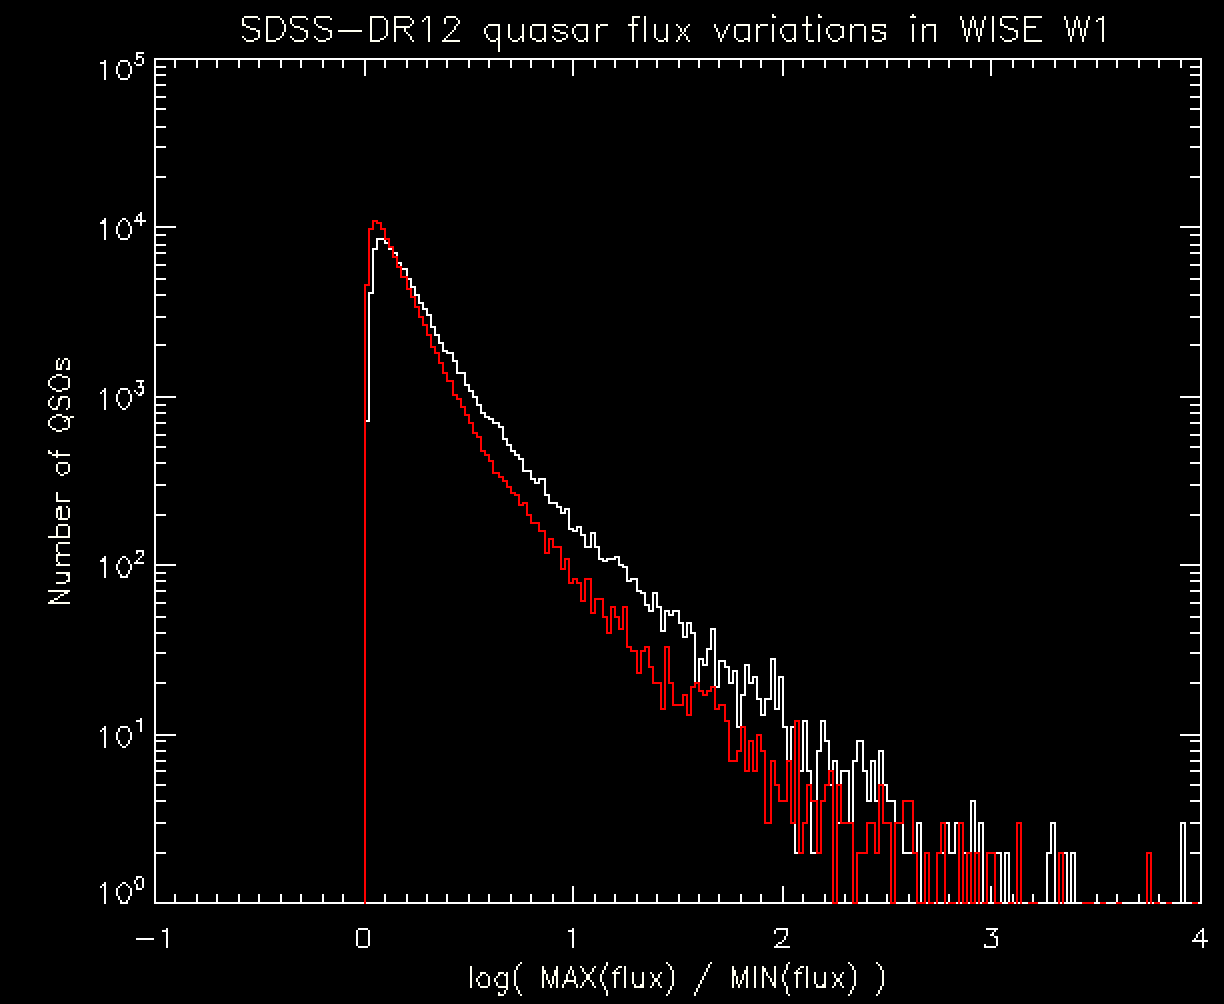
\includegraphics[width=8.00cm, height=7.50cm, trim=0.0cm 0.0cm 0.0cm 0.0cm, clip]
  {fig1.png}
  \centering
  % \vspace{-16pt}
  \caption[]{
    %% {\bf All from DJS's email:} 
    The distribution of the maxima and
    minima flux in $W1$ for the $\sim$240k high-confidence quasars in the
    SDSS-III: BOSS DR12.  The red distribution is if one replaces fluxes
    with a mean flux$+$measurement error for each observation.  Note,
    since the log is being plotted, the difference between the two lines
    shows a significant variable population.  There are $\sim$1000 quasars
    where the $W1$ flux varies by more than a factor of 2 with a $>5$
    sigma confidence.  Some have a poor $\chi{^2}$ fits.
  }
  \label{fig:maxminflux}
\end{figure}
The distribution of the maxima and minima flux in $W1$ for the
$\sim$240k high-confidence quasars in the SDSS-III: BOSS DR12 is given
in Figure~\ref{fig:maxminflux}.

\begin{figure}
  %% trim=l b r t 
  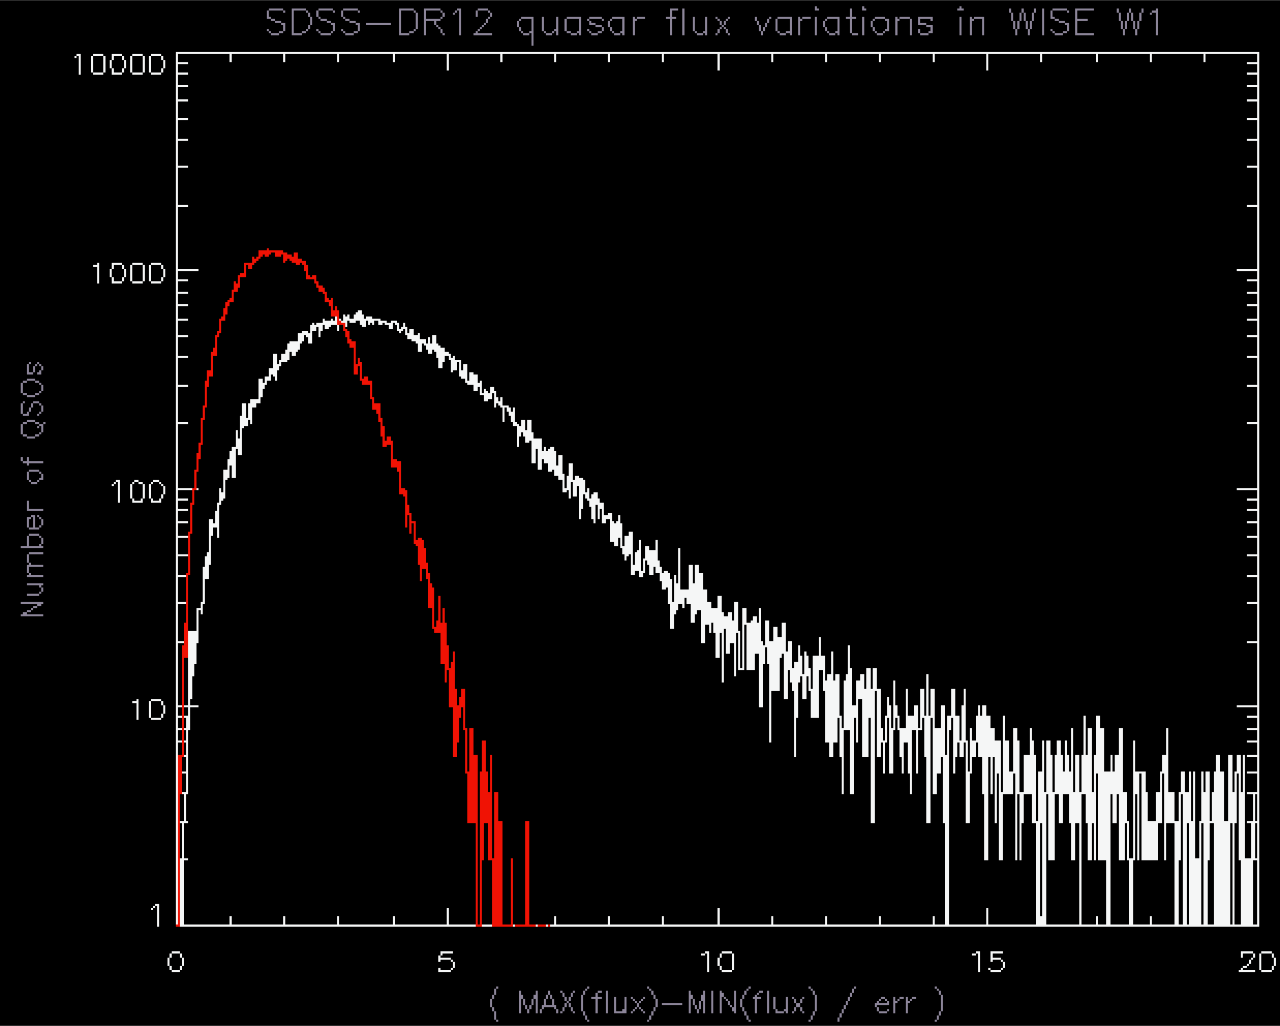
\includegraphics[width=8.00cm, height=7.50cm, trim=0.0cm 0.0cm 0.0cm 0.0cm, clip]
  {fig2.png}
  \centering
  % \vspace{-16pt}
  \caption[]{
%    {\bf All from DJS's 2nd email:} 
    Here, ``err'' is the quadrature sum of the errors at the minimum and maximum fluxes.
    The red histogram is the expected distribution if these objects had no variability, 
    and the errors were normally-distributed for each of the epochs.
    This shows that $\sim6,000$ quasars are $>10\sigma$ detections of variability in W1.
    % Though I still havent done this carefully enough to reject the poor chi^2 in individual WISE fits, etc.
  }
  \label{fig:maxmin_err}
\end{figure}
\subsection{``False Postive Checks''}
Figure~\ref{fig:maxmin_err} is the distribution of (max-min)/error in
the MIR fluxes.  (Should also be looking at the SDSS stars as a
control sample).  The WISE magnitude
range for those stars will be quite different, though, since they have
the same optical magnitude range but are fainter in WISE.

%%  This is text from Aaron's email from 15th Feb, 2017, sent to Daniel, 
%%  for the WISE J1052+1519 outline/paper
W1 and W2 lightcurves for $\sim$200,000 SDSS spectroscopic quasars
were extracted from Data Release 3 (DR3) of the Dark Energy Camera
Legacy Survey (DECaLS). These light curves span from the beginning of
the WISE mission (2010 January) through the first-year of NEOWISER
operations (2014 December). In detail, the W1/W2 light curves are
obtained by performing forced photometry at the locations of
DECam-detected optical sources. This forced photometry is performed on
time-resolved unWISE coadds, each of which represents a stack with
depth of coverage $\sim$12 exposures. A given sky location is observed
by WISE for $\sim$1 day once every six months, which means that our
forced photometry light curves typically have four coadd epochs
available. Coadd epochs of a given object are separated by a minimum
of six months and a maximum of four years. Our coaddition removes the
possibility of probing variability on $\lesssim$1 day time scales, but
it allows us to push $\sim$1.4 magnitudes deeper than individual
exposures while removing virtually all single-exposure artifacts
(e.g. cosmic rays and satellites).

$\sim$30,000 of the SDSS quasars with such W1/W2 lightcurves available
are ``IR-bright'', in the sense that they are above both the W1 and W2
single exposure thresholds and therefore detected at very high
significance in our coadds. For this ensemble of objects, the typical
variation in each quasar's measured (W1-W2) color is 0.06 magnitudes,
which includes statistical and systematic errors expected to
contribute variations at the few hundredths of a mag level. The
typical measured single-band scatter is 0.07 magnitudes in each of W1
and W2. A full characterization of the typical mid-IR quasar
variability will be presented separately (Ross et al., in
preparation).

We undertook a search for extreme outliers relative to these trends.
Specifically, we selected objects with the following characteristics.

% itemize type stuff
\begin{itemize}
\item Monotonic variation in both W1 and W2.
\item W1 versus W2 \textit{flux} correlation coefficient $>$0.9.
\item $>0.5$ mag peak-to-peak variation in either W1 or W2.
\end{itemize}

This yielded a sample of 248 sources. 31 of these are assumed to be blazars 
due to the presence of FIRST radio counterparts. Another 22 are outside of the 
FIRST  footprint, leaving 195 quasars in our IR-variable sample. We randomly 
selected five of these objects for follow-up spectroscopy with Palomar DBSP on
the night of 30 January 2017. WISE J1052+1519, one of these five, 
faded by 0.75 (0.9) mags in W1 (W2), and thus became 0.15 mags bluer in 
(W1-W2), making it a significant outlier in both single-band and IR color 
variability.

A link to the key properties of our sample can be found here:
\href{http://portal.nersc.gov/project/cosmo/temp/ameisner/qso\_pages\_v01/}
{\tt qso\_pages\_v01} and the links to the catalogs are given here: 
\href{http://portal.nersc.gov/project/cosmo/temp/ameisner/dr3_wise_lc_sample.fits.gz}{{\tt dr3\_wise\_lc\_sample.fits.gz}} and here:
\href{http://portal.nersc.gov/project/cosmo/temp/ameisner/dr3_wise_lc_metrics_all_qso.fits.gz}{{\tt dr3\_wise\_lc\_sample.fits.gz}}. 
The first catalog has 248 rows, which are the selected highly
IR-variable sample of objects.  The second catalog is the full
\hbox{200 622} quasar sample quasars that have ``good'' WISE light
curves available in DECaLS DR3. In each file, there are 3 extensions:
ex = 0 -- WISE light curve summary metrics; ex = 1 -- DECaLS DR3
Tractor data for each object; ex = 2 -- SDSS data for each object.



%%%%%%%%%%%%%%%%%%%%%%%%%%%%%%%%%%%%%%%%%%%%%%%%%%%%%%%%%%%%%%
%%%%%%%%%%%%%%%%%%%%%%%%%%%%%%%%%%%%%%%%%%%%%%%%%%%%%%%%%%%%%%
%%
%%     S E C T I O N     3      S E C T I O N     3       S E C T I O N     3       S E C T I O N     3  
%%     S E C T I O N     3      S E C T I O N     3       S E C T I O N     3       S E C T I O N     3  
%%     S E C T I O N     3      S E C T I O N     3       S E C T I O N     3       S E C T I O N     3  
%%
%%%%%%%%%%%%%%%%%%%%%%%%%%%%%%%%%%%%%%%%%%%%%%%%%%%%%%%%%%%%%%
%%%%%%%%%%%%%%%%%%%%%%%%%%%%%%%%%%%%%%%%%%%%%%%%%%%%%%%%%%%%%%
\begin{figure}
  %% trim=l b r t 
  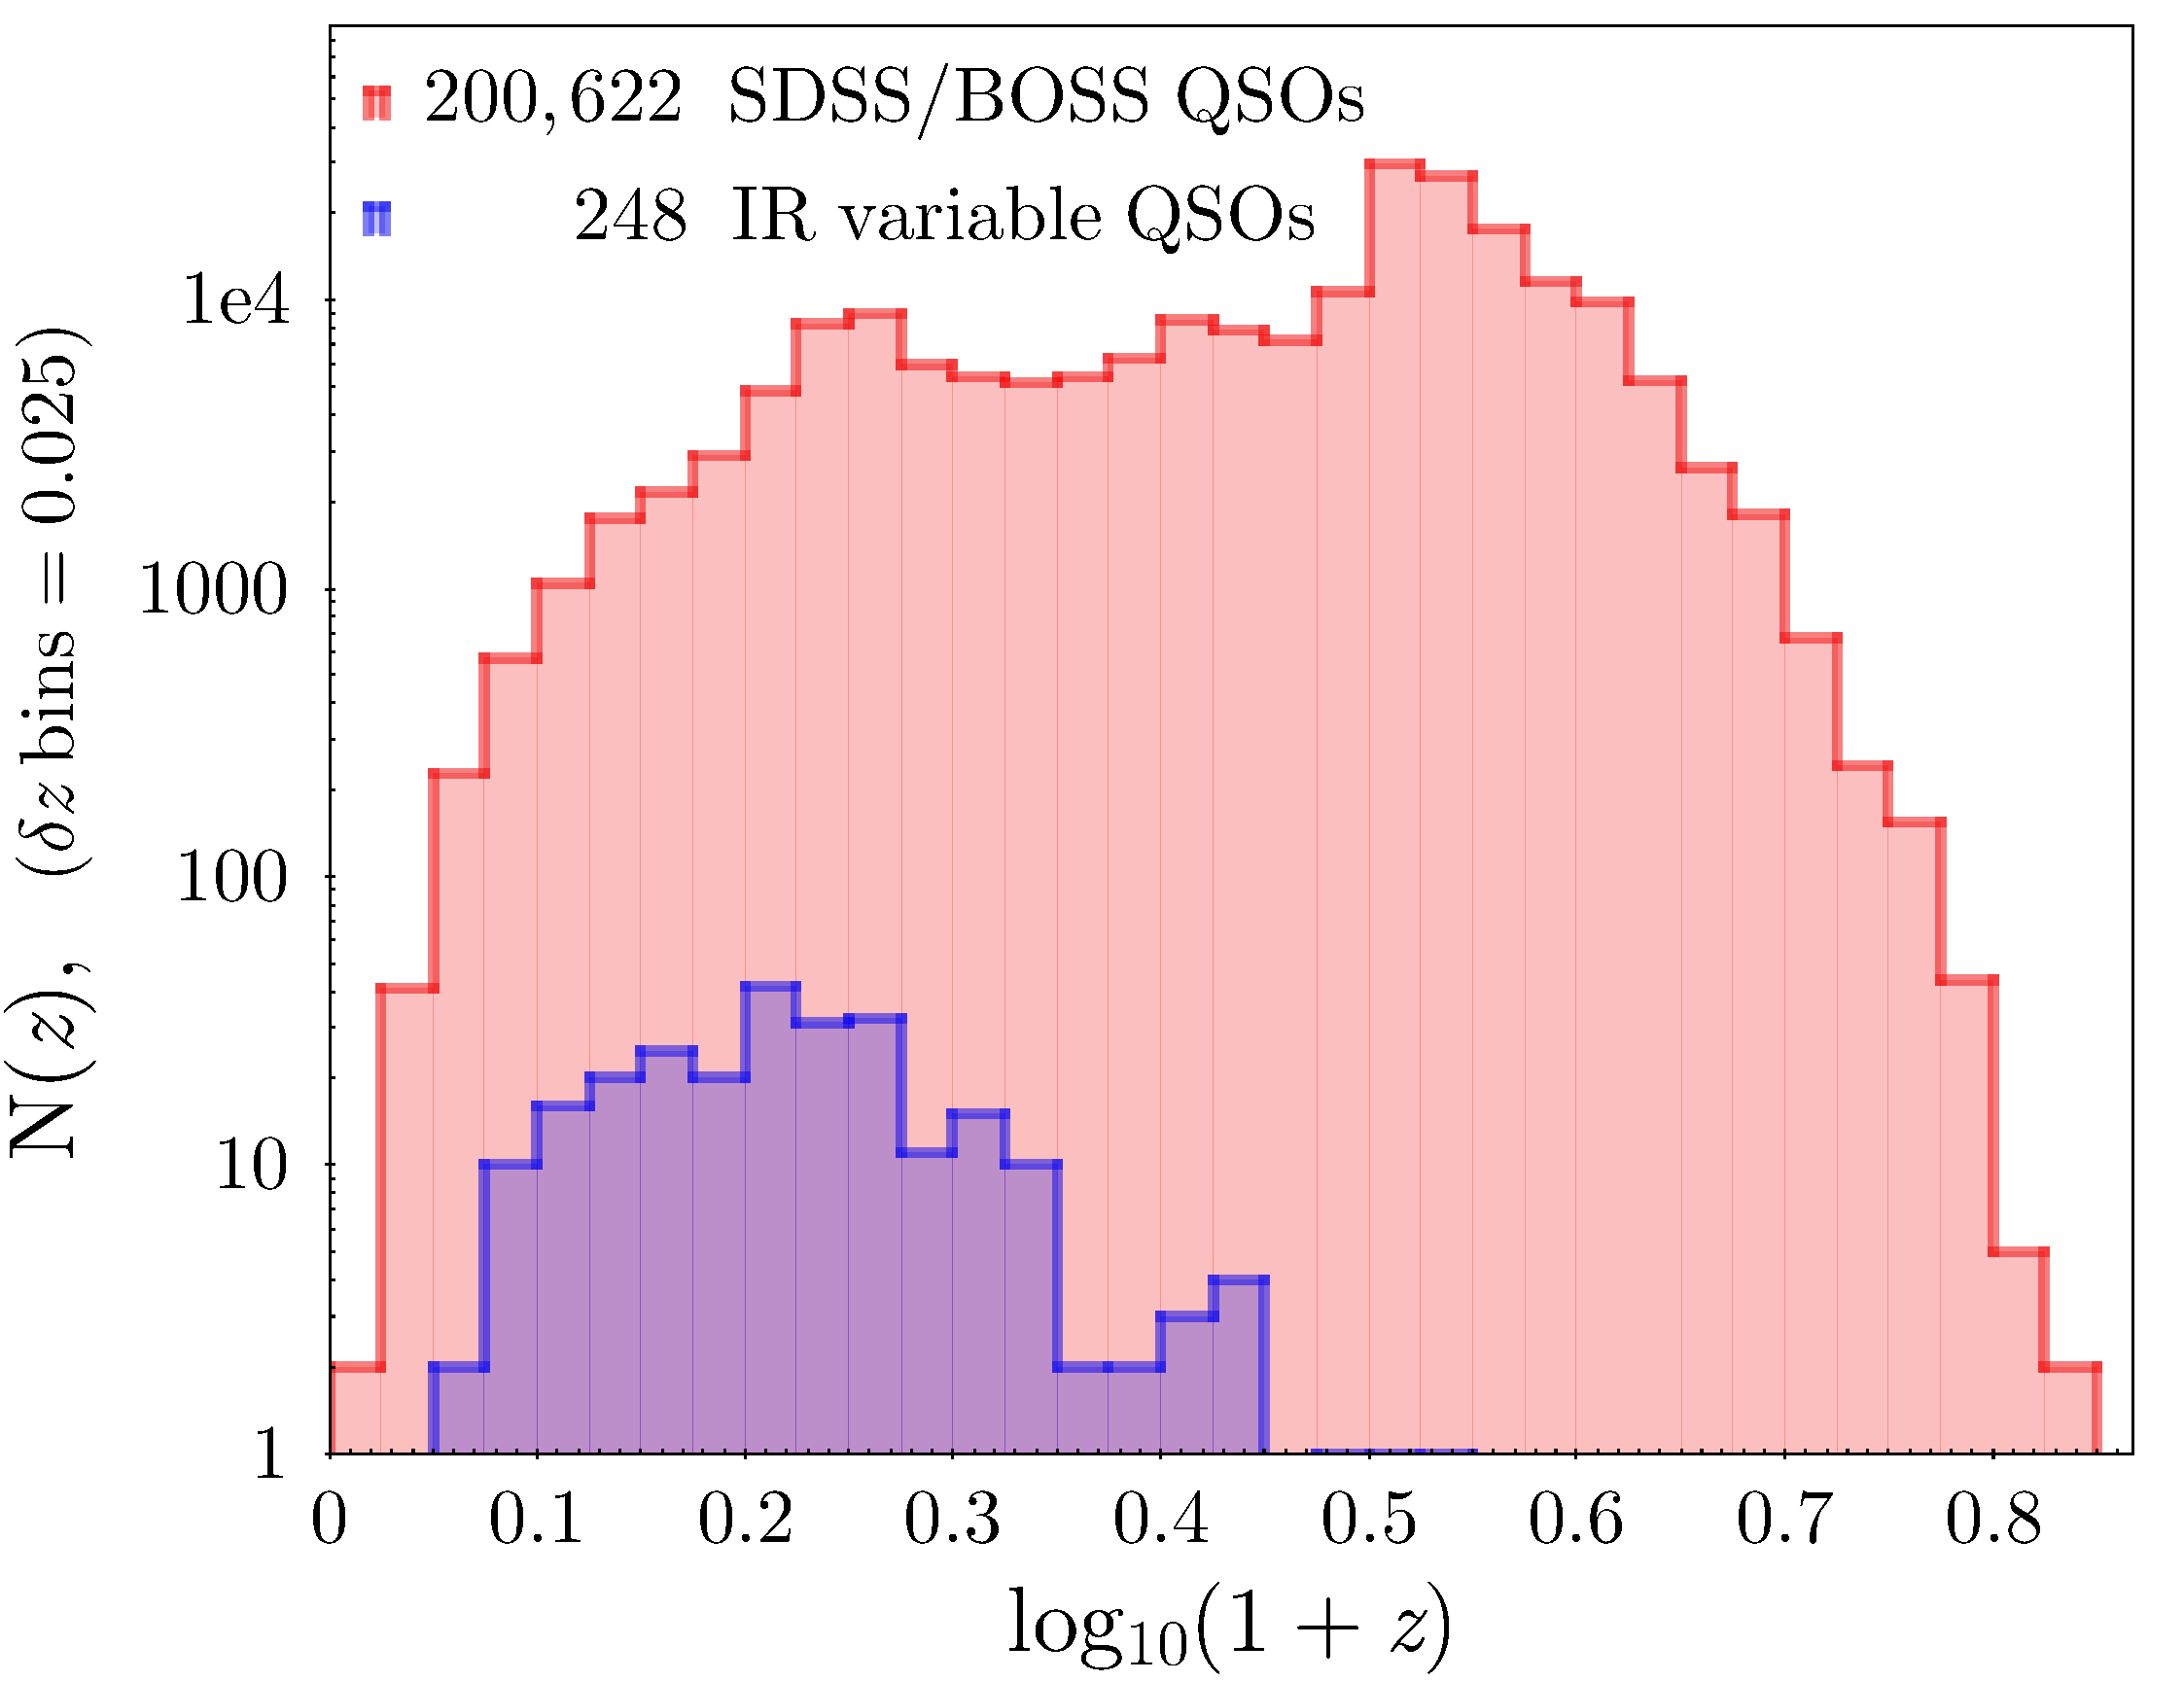
\includegraphics[width=8.20cm, height=7.00cm, 
  trim=0.0cm 0.0cm 0.1cm 0.0cm, clip]
  {../plots/Nofz/Nofz_20170331.pdf}
  \centering
  % \vspace{-16pt}
  \caption[]{The the variations in $(W1-W2)$ color using
    $\sim$37,500 data points from $\sim$9000 bright quasars.
    Overplotted is a Gaussian distribution, centered at -3.8 mmag 
    and with standard deviation of 0.06 mags (with a fit-by-eye ;-).}
  \label{fig:Nofz}
\end{figure}

\section{Results: General Population}
Starting from the $\approx$200,000 object parent quasar sample, 
and employing the selections as described above, we generate a catalog 
of 248 objects. 
Some general properties include:
\begin{itemize}
    \item{
        The redshift distribution of the IR-variable sample of objects
        being at generally lower redshift than the parent sample, but
        extending to relatively high-$z$ - see Figure~\ref{fig:Nofz}}; 
    \item{221 (89\%) of the sample have falling IR light-curves.}
    \item{The extremely IR variable QSOs generally have the same
      optical colors as the parent population, see
      Figures~\ref{fig:ugriz_colorcolor} and \ref{fig:grz_colorcolor}.}
\end{itemize}
The $N(z)$ redshift distributions are shown in Figure~\ref{fig:Nofz}
with the parent sample the blue histogram and the IR-variable sample
the red histogram.

Lorem ipsum dolor sit amet, consectetur adipiscing elit. Aliquam porta
sodales est, vel cursus risus porta non. Vivamus vel pretium
velit. Sed fringilla suscipit felis, nec iaculis lacus convallis
ac. Fusce pellentesque condimentum dolor, quis vehicula tortor
hendrerit sed. Class aptent taciti sociosqu ad litora torquent per
conubia nostra, per inceptos himenaeos. Etiam interdum tristique diam
eu blandit. Donec in lacinia libero.

    \begin{figure}
      %% trim=l b r t 
      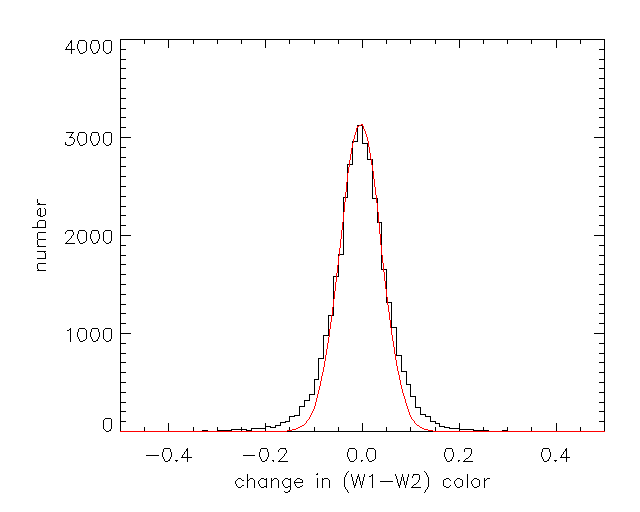
\includegraphics[width=7.20cm, height=7.20cm, 
      trim=0.0cm 0.0cm 0.0cm 0.0cm, clip]
      {../plots/w1w2_color_variation.png}
      \centering
      % \vspace{-16pt}
      \caption[]{The the variations in $(W1-W2)$ color using
        $\sim$37,500 data points from $\sim$9000 bright quasars.
        Overplotted is a Gaussian distribution, centered at -3.8 mmag 
        and with standard deviation of 0.06 mags (with a fit-by-eye ;-).}
      \label{fig:w1w2_color_variation}
    \end{figure}
    \subsection{Color Changes}
    Figure~\ref{fig:w1w2_color_variation} shows the variations in the
    $(W1-W2)$ color, which is pretty narrow. Overplotted is a Gaussian
    distribution, centered at -3.8 mmag and with standard deviation of
    0.06 mags.
    
    This histogram includes $\sim$37,500 data points from $\sim$9000
    bright quasars, that is, brighter than single-exposure detection limit
    in both W1 and W2. {\it NPR: It'd be very most awesome if we could
      show a W1W2W3 RGB image of a quasar changing color!!!}
    
    \begin{figure}
      %% trim=l b r t 
      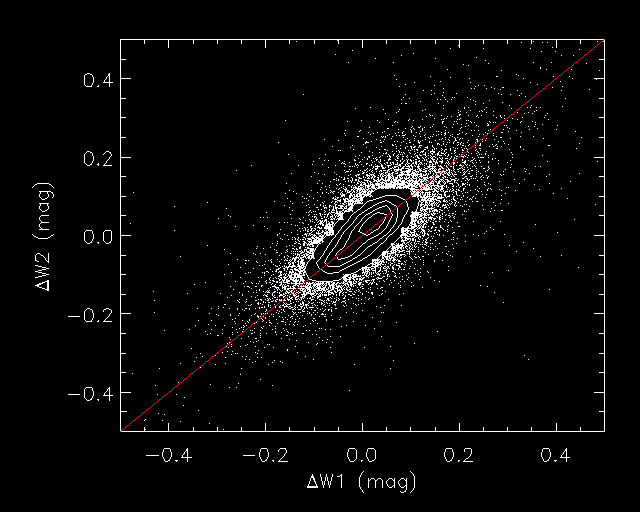
\includegraphics[width=7.00cm, height=7.00cm, 
      trim=0.0cm 0.0cm 0.0cm 0.0cm, clip]
      {scatter_dW1_dW2.png}
      \centering
      % \vspace{-16pt}
      \caption[]{The the variations in $(W1-W2)$ color using
        $\sim$37,500 data points from $\sim$9000 bright quasars. Overplotted
        is a Gaussian distribution, centered at -3.8 mmag and with standard
        deviation of 0.06 mags.}
      \label{fig:scatter_dW1_dW2}
    \end{figure}
    Figure~\ref{fig:scatter_dW1_dW2} has the same data as
    Fig~\ref{fig:w1w2_color_variation}, now in a scatterplot of
    $\Delta(W1)$ versus $\Delta(W2$). There is clearly some variation, and
    it is well-correlated between W1 and W2. The red line is $x=y$. 
    (I would guess this is real variation, but I'm still a little bit scared that
    you could have e.g. correlated background level issues in the coadds
    that imprint onto the fluxes.)


    \begin{figure*}
      %% trim=l b r t 
      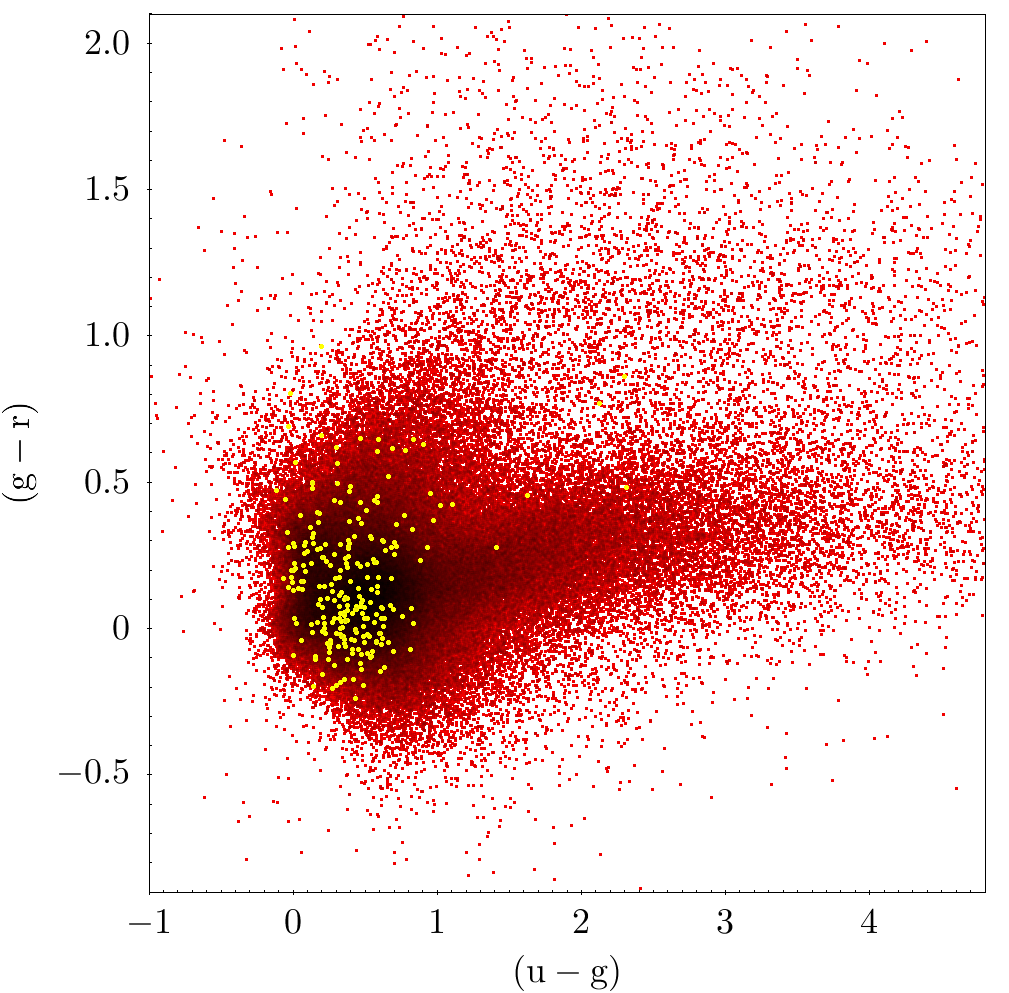
\includegraphics[width=5.50cm, height=5.50cm, trim=0.0cm 0.0cm 0.0cm 0.0cm, clip]
      {../color_color/colorcolor_ugr_topcat.png}
      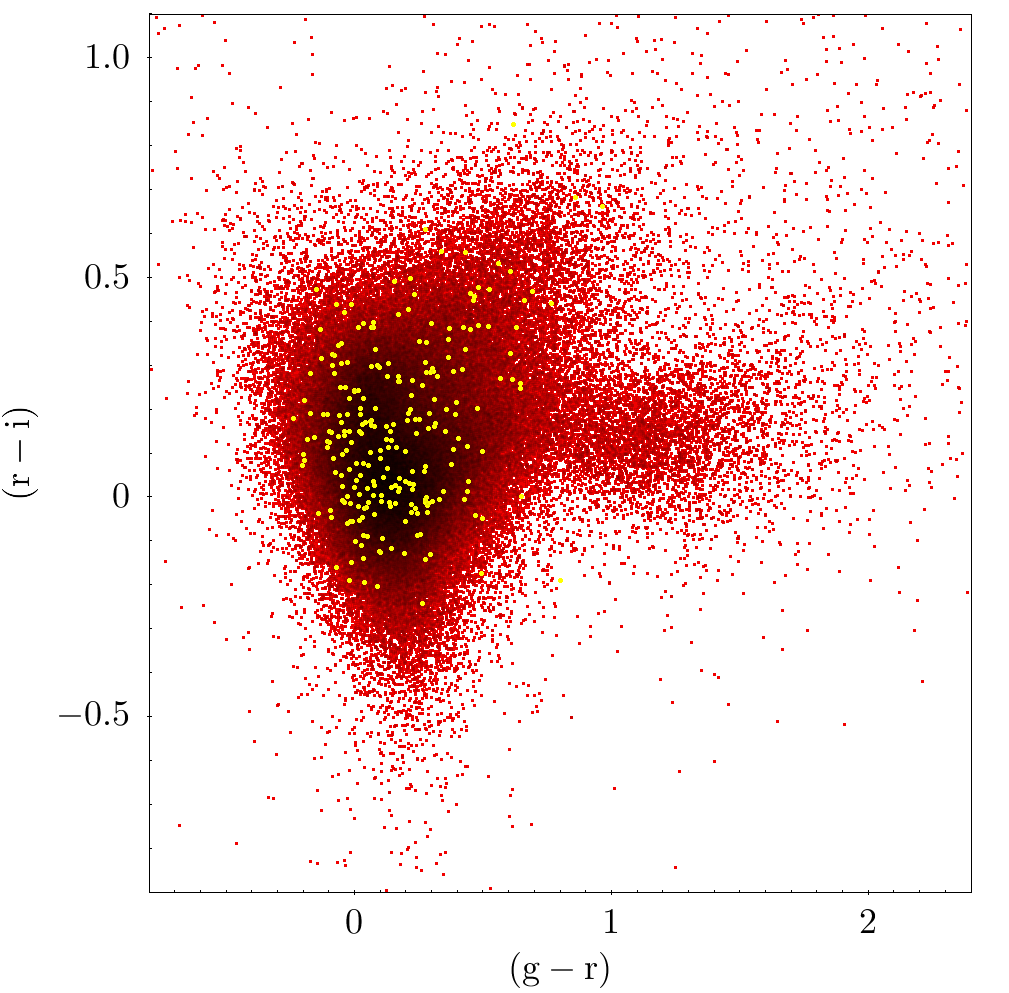
\includegraphics[width=5.50cm, height=5.50cm, trim=0.0cm 0.0cm 0.0cm 0.0cm, clip]
      {../color_color/colorcolor_gri_topcat.png}
      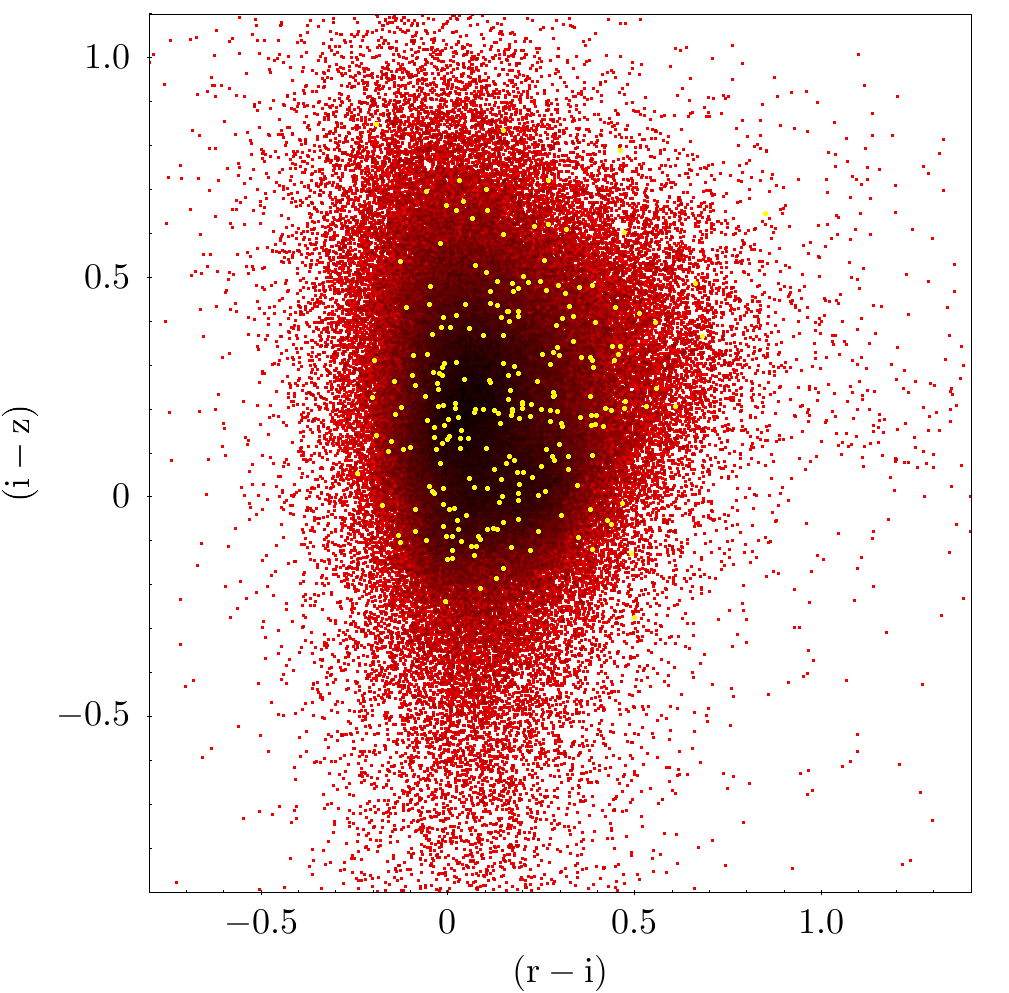
\includegraphics[width=5.50cm, height=5.50cm, trim=0.0cm 0.0cm 0.0cm 0.0cm, clip]
      {../color_color/colorcolor_riz_topcat.png}
      \centering
      % \vspace{-16pt}
      \caption[]{The $ugriz$ color-color plots for the full 200k
        super-sample (red points) and the 248 extreme IR variables (yellow
        dots).}
      \label{fig:ugriz_colorcolor}
    \end{figure*}
    Etiam mollis viverra nisi eget aliquet. Aliquam erat volutpat. Vivamus
    tristique, nisl eu malesuada semper, libero tortor convallis elit, a
    scelerisque orci nisi lacinia turpis. In lacinia ultrices
    volutpat. Proin ultrices luctus tellus, in placerat eros tincidunt
    id. Ut varius iaculis quam in consequat. Nulla nec orci est, sit amet
    pellentesque nisl. Mauris non cursus lectus. Praesent placerat leo vel
    erat gravida lacinia. Donec vehicula consectetur lectus vitae
    luctus. Praesent nisl justo, laoreet elementum facilisis vel,
    tristique ac enim. Etiam vel quam ut quam eleifend
    tincidunt. Suspendisse sit amet eros vel elit ullamcorper
    laoreet. Etiam venenatis sodales turpis, nec lacinia ligula hendrerit
    nec. Nam eu vulputate purus. Quisque facilisis congue metus, sed
    imperdiet lorem rhoncus sit amet.
    
    \begin{figure}
      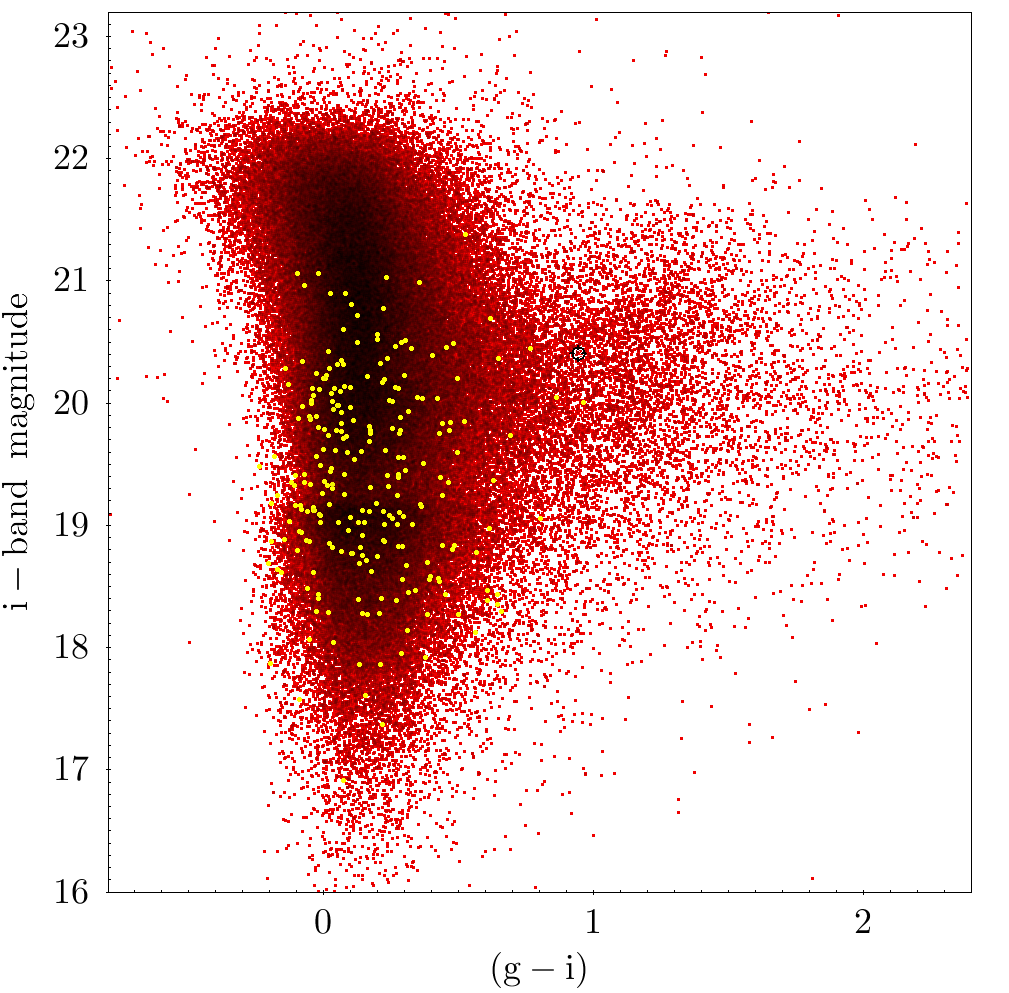
\includegraphics[width=7.00cm, height=7.00cm, trim=0.0cm 0.0cm 0.0cm 0.0cm, clip]
      {../color_color/colormag_gr_imag_topcat.png}
      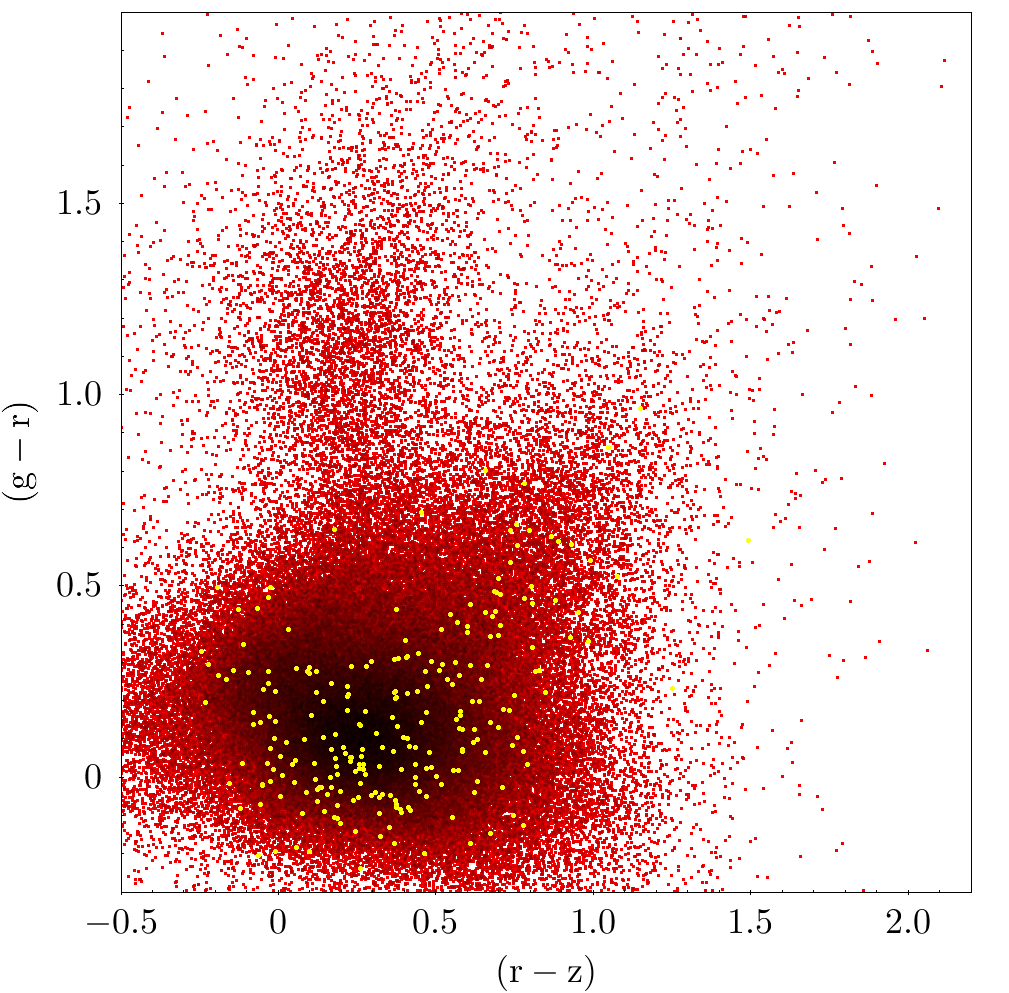
\includegraphics[width=7.00cm, height=7.00cm, trim=0.0cm 0.0cm 0.0cm 0.0cm, clip]
      {../color_color/colormag_grz_topcat.png}
      \centering
      % \vspace{-16pt}
      \caption[]{The color-mag and $grz$ color-color plots for the full 200k super-sample (red points) 
        and the 248 extreme IR variables (yellow).}
      \label{fig:grz_colorcolor}
    \end{figure}

    \subsection{Changes in color: One IR Variable population or two?}
    Turpis tincidunt quam consectetur non suscipit tellus placerat. Etiam
    sit amet justo condimentum sem scelerisque pharetra. Nullam sit amet
    neque eget quam tempor consectetur vel vitae massa. Nunc porttitor,
    quam in tempor pharetra, leo libero eleifend mi, ac ornare nibh eros
    vel purus. Pellentesque lobortis enim metus.

    %\begin{table}
\begin{tabular}{cccccccccccccccccc}
SDSSJ & RA & DEC & Z & PLATE & FIBER & MJD & PEARSON\_R & BEST\_FLUX\_W1 & BEST\_FLUX\_W2 & FLUX\_MAX\_W1 & FLUX\_MAX\_W2 & FLUX\_MIN\_W1 & FLUX\_MIN\_W2 & MAG\_RANGE\_W1 & MAG\_RANGE\_W2 & RISING\_W1 & RISING\_W2 \\
000920.76+033021.7 & 2.33654086687 & 3.50603303134 & 0.432505905628 & 4297 & 196 & 55806 & 0.999489 & 72.078 & 94.7315 & 86.1033 & 114.478 & 56.8723 & 69.1232 & 0.450297 & 0.547747 & 0 & 0 \\
001053.44+231604.9 & 2.72267621623 & 23.2680334774 & 0.752258002758 & 6880 & 202 & 56543 & 0.985843 & 95.3537 & 127.092 & 108.239 & 148.875 & 77.9631 & 93.4501 & 0.356233 & 0.505604 & 0 & 0 \\
001130.39+005751.8 & 2.87665180272 & 0.964415750637 & 1.49 & 4217 & 946 & 55478 & 0.999884 & 132.038 & 219.862 & 273.697 & 430.71 & 25.4144 & 36.0975 & 2.58047 & 2.69177 & 0 & 0 \\
001238.49+230328.8 & 3.16041434409 & 23.0580121564 & 0.872348427773 & 6881 & 359 & 56540 & 0.997853 & 43.7786 & 63.439 & 49.3492 & 75.5982 & 36.4012 & 47.1703 & 0.33041 & 0.512106 & 0 & 0 \\
001254.25+193707.9 & 3.22604854198 & 19.6188883647 & 0.503228604794 & 6174 & 732 & 56243 & 0.941403 & 37.1537 & 52.2155 & 46.4315 & 76.2861 & 25.0222 & 28.8935 & 0.671217 & 1.05412 & 0 & 0 \\
001539.99+170040.5 & 3.91663820339 & 17.0112615148 & 1.7200088501 & 6111 & 100 & 56270 & 0.988381 & 38.0622 & 63.6586 & 69.5563 & 122.872 & 22.1566 & 29.1941 & 1.24208 & 1.5604 & 0 & 0 \\
001702.88+250559.6 & 4.26201771268 & 25.09990315 & 0.243872866035 & 6279 & 660 & 56243 & 0.999826 & 92.0064 & 120.638 & 129.719 & 177.559 & 70.6003 & 91.4998 & 0.660491 & 0.719806 & 1 & 1 \\
001744.44+253123.6 & 4.43518860333 & 25.523231208 & 0.758191466331 & 6279 & 676 & 56243 & 0.970858 & 52.0593 & 44.8865 & 57.9811 & 63.8945 & 46.5449 & 33.3697 & 0.238536 & 0.705278 & 1 & 1 \\
002125.18+231025.1 & 5.35494705482 & 23.1736602346 & 0.815230727196 & 6882 & 394 & 56541 & 0.996137 & 49.8901 & 60.3679 & 60.8984 & 78.4536 & 41.2784 & 44.3163 & 0.422208 & 0.620123 & 0 & 0 \\
002810.91+262510.7 & 7.04547508037 & 26.4196389292 & 0.862826228142 & 6281 & 745 & 56295 & 0.976747 & 32.2795 & 46.7901 & 38.4635 & 58.1213 & 26.6385 & 35.2498 & 0.398848 & 0.542946 & 0 & 0 \\
002917.29+024619.8 & 7.32205987295 & 2.77217878694 & 0.726760387421 & 4301 & 173 & 55810 & 0.999056 & 85.418 & 107.951 & 109.483 & 133.09 & 58.8954 & 76.9684 & 0.673162 & 0.594582 & 0 & 0 \\
003625.84+011258.4 & 9.10767697614 & 1.21622940345 & 0.86627805233 & 4221 & 862 & 55443 & 0.932855 & 28.9693 & 47.9417 & 34.3939 & 64.4323 & 21.9838 & 28.3624 & 0.485944 & 0.890903 & 0 & 0 \\
003859.67-034000.7 & 9.74864452147 & -3.66688077687 & 0.865895032883 & 7040 & 668 & 56574 & 0.942636 & 63.541 & 102.622 & 76.7064 & 129.787 & 53.3356 & 76.4114 & 0.394537 & 0.575183 & 0 & 0 \\
004530.42+125403.3 & 11.3767895588 & 12.9009196152 & 0.655647099018 & 6202 & 156 & 56266 & 0.991671 & 51.9636 & 92.4265 & 66.3298 & 110.751 & 41.26 & 71.3809 & 0.515448 & 0.476914 & 0 & 0 \\
004653.63+053406.8 & 11.7234836086 & 5.56855949673 & 0.790611922741 & 4419 & 10 & 55867 & 0.963992 & 78.4327 & 74.5741 & 84.6877 & 87.0422 & 67.581 & 54.3668 & 0.244989 & 0.51099 & 0 & 0 \\
010044.21-040810.9 & 15.1842109756 & -4.13638255411 & 0.566544234753 & 7043 & 764 & 56576 & 0.970251 & 93.7984 & 104.291 & 103.413 & 125.567 & 65.2189 & 58.7034 & 0.500501 & 0.825527 & 0 & 0 \\
011118.69+235808.8 & 17.8278966604 & 23.9691236157 & 0.90282279253 & 5126 & 542 & 55923 & 0.976393 & 42.7196 & 85.2924 & 61.7386 & 110.599 & 28.3509 & 57.3196 & 0.844974 & 0.713621 & 0 & 0 \\
012141.59+114950.4 & 20.4233031661 & 11.8306723861 & 0.571315348148 & 4669 & 694 & 55831 & 0.9944 & 894.581 & 1266.96 & 1100.81 & 1606.28 & 730.16 & 819.475 & 0.445733 & 0.730712 & 0 & 0 \\
021104.17-045325.0 & 32.7674053995 & -4.89030505937 & 0.525170624256 & 7238 & 981 & 56660 & 0.974047 & 58.9339 & 78.8442 & 78.3803 & 103.41 & 42.4 & 50.5404 & 0.667102 & 0.777304 & 0 & 0 \\
021740.47-035029.3 & 34.4186466932 & -3.8414779352 & 1.05192315578 & 7237 & 946 & 56662 & 0.90725 & 34.4437 & 66.5459 & 44.9415 & 86.8616 & 24.8256 & 38.9084 & 0.644371 & 0.87196 & 0 & 0 \\
024026.72+014255.9 & 40.111353931 & 1.71552955684 & 0.842329204082 & 4261 & 300 & 55503 & 0.946861 & 51.1516 & 67.7502 & 59.1402 & 86.8287 & 40.4491 & 45.5062 & 0.412434 & 0.701482 & 0 & 0 \\
083750.72+063633.6 & 129.46136597 & 6.60934044369 & 0.634521722794 & 4903 & 683 & 55927 & 0.98926 & 57.17 & 75.9919 & 77.8332 & 123.011 & 33.0977 & 39.2478 & 0.928417 & 1.24032 & 1 & 1 \\
083859.40+171510.5 & 129.747501013 & 17.2529354994 & 0.696680605412 & 5286 & 548 & 56225 & 0.996698 & 61.2459 & 59.0902 & 67.2714 & 71.9259 & 54.9095 & 43.5961 & 0.220456 & 0.543594 & 1 & 1 \\
084118.14+015406.6 & 130.325624207 & 1.90183929163 & 0.426525354385 & 4793 & 906 & 55648 & 0.9819 & 52.9636 & 64.4085 & 62.4709 & 79.9464 & 46.1275 & 44.7533 & 0.329296 & 0.629934 & 0 & 0 \\
085036.06+040810.4 & 132.650290161 & 4.13624621005 & 0.455819457769 & 3814 & 522 & 55535 & 0.999479 & 110.361 & 158.51 & 145.695 & 189.459 & 79.6408 & 122.396 & 0.655773 & 0.474367 & 0 & 0 \\
090343.63+102305.3 & 135.931804511 & 10.3848111529 & 0.634052336216 & 5296 & 194 & 55922 & 0.999098 & 191.664 & 229.798 & 220.298 & 289.624 & 157.588 & 177.237 & 0.363718 & 0.5332 & 1 & 1 \\
090807.72+120010.3 & 137.032171668 & 12.0028850696 & 0.909615337849 & 5298 & 130 & 55979 & 0.955401 & 38.1076 & 42.2431 & 43.0314 & 60.5748 & 33.2637 & 31.9068 & 0.279536 & 0.696021 & 1 & 1 \\
092118.48+295735.2 & 140.327038653 & 29.9597852233 & 0.761953532696 & 5803 & 520 & 56272 & 0.949301 & 50.6972 & 99.4302 & 66.2327 & 134.609 & 34.6429 & 70.5513 & 0.703644 & 0.701421 & 0 & 0 \\
092750.78+200303.0 & 141.961601946 & 20.0508375164 & 0.941165745258 & 5767 & 840 & 56245 & 0.968256 & 31.4169 & 42.7301 & 38.9133 & 61.375 & 25.8248 & 31.2733 & 0.445151 & 0.732043 & 1 & 1 \\
093148.13+234837.0 & 142.950567427 & 23.8103001882 & 0.891499459743 & 5789 & 584 & 56246 & 0.987802 & 41.4461 & 70.0891 & 49.6046 & 88.4027 & 34.6404 & 47.0694 & 0.389846 & 0.684319 & 0 & 0 \\
094554.40-002026.2 & 146.476672377 & -0.340617322862 & 0.6825953722 & 3827 & 426 & 55565 & 0.974253 & 27.3048 & 43.1761 & 34.1759 & 56.4227 & 21.2697 & 30.4543 & 0.514898 & 0.669513 & 0 & 0 \\
095538.30+241321.6 & 148.909599109 & 24.2226903891 & 0.800511419773 & 5787 & 818 & 56254 & 0.973565 & 49.7672 & 71.7687 & 57.2151 & 94.3192 & 45.141 & 56.9604 & 0.25735 & 0.547568 & 0 & 0 \\
100818.54+264434.9 & 152.077280407 & 26.7430444161 & 0.734007418156 & 6470 & 472 & 56334 & 0.976926 & 64.3928 & 69.0528 & 72.3229 & 82.9868 & 57.1879 & 49.1256 & 0.254929 & 0.569253 & 0 & 0 \\
101216.39+231214.6 & 153.068293641 & 23.2040630428 & 0.749825954437 & 6458 & 736 & 56274 & 0.994434 & 126.145 & 202.8 & 202.212 & 302.709 & 73.3475 & 107.271 & 1.10105 & 1.12636 & 0 & 0 \\
101337.44+302107.9 & 153.40601646 & 30.3522165184 & 2.0 & 6469 & 932 & 56328 & 0.999679 & 41.7274 & 125.2 & 61.2895 & 188.911 & 25.282 & 64.1661 & 0.961438 & 1.17238 & 0 & 0 \\
101403.18+251608.6 & 153.513277422 & 25.2690779765 & 1.26332890987 & 6465 & 540 & 56279 & 0.992443 & 30.1034 & 51.1285 & 34.9522 & 58.7646 & 20.7607 & 35.3137 & 0.565582 & 0.552933 & 0 & 0 \\
102136.98+004613.4 & 155.404095536 & 0.770406255336 & 0.75149589777 & 3831 & 840 & 55543 & 0.944624 & 63.3674 & 71.0582 & 73.8712 & 94.4169 & 53.4216 & 50.5478 & 0.351896 & 0.678369 & 1 & 1 \\
102221.32+102623.7 & 155.588848588 & 10.4399373421 & 0.6552490592 & 5341 & 531 & 55931 & 0.966297 & 67.8476 & 98.1301 & 77.949 & 120.689 & 56.1827 & 75.4249 & 0.35552 & 0.510386 & 0 & 0 \\
102357.34+223512.6 & 155.988939085 & 22.5868549001 & 1.091 & 6424 & 234 & 56272 & 0.995362 & 15.9029 & 33.8807 & 26.5129 & 48.6402 & 5.55415 & 18.5863 & 1.6971 & 1.04451 & 0 & 0 \\
102639.42+274931.5 & 156.664274419 & 27.8254297012 & 0.792031943798 & 6463 & 884 & 56340 & 0.935369 & 38.342 & 49.1702 & 48.0767 & 58.5195 & 30.0381 & 32.9406 & 0.510654 & 0.623921 & 0 & 0 \\
102700.25+290938.2 & 156.751082432 & 29.1606259158 & 0.515792071819 & 6456 & 351 & 56339 & 0.943372 & 37.7201 & 58.5007 & 48.0875 & 70.0108 & 28.9467 & 40.7051 & 0.551085 & 0.588791 & 0 & 0 \\
102834.03-023659.6 & 157.141820386 & -2.6165715345 & 0.470204979181 & 3785 & 424 & 55273 & 0.999997 & 1479.26 & 2549.87 & 4693.07 & 6956.07 & 113.66 & 185.912 & 4.03962 & 3.93264 & 0 & 0 \\
103931.57+231922.1 & 159.881574851 & 23.3228246525 & 1.159 & 6426 & 598 & 56334 & 0.979588 & 32.48 & 64.052 & 39.4171 & 76.9173 & 24.4834 & 40.0096 & 0.517033 & 0.709651 & 0 & 0 \\
104355.02+232200.4 & 160.97926975 & 23.3667788211 & 0.888 & 6426 & 834 & 56334 & 0.993813 & 64.3281 & 83.7522 & 73.0809 & 99.7407 & 52.1758 & 59.0337 & 0.365838 & 0.569431 & 0 & 0 \\
110106.26+040747.1 & 165.276120081 & 4.12976474608 & 0.721132516861 & 4771 & 690 & 55925 & 0.999884 & 74.4214 & 108.224 & 95.3457 & 135.752 & 51.9232 & 84.8653 & 0.65985 & 0.510037 & 1 & 1 \\
110305.62+225730.7 & 165.773422765 & 22.9585550062 & 1.09459173679 & 6418 & 42 & 56354 & 0.991004 & 47.626 & 71.6083 & 57.9683 & 85.2434 & 38.3065 & 53.6424 & 0.449795 & 0.502882 & 0 & 0 \\
110427.76+225945.4 & 166.115696692 & 22.9959698838 & 0.655519068241 & 6428 & 789 & 56279 & 0.978792 & 57.8673 & 78.7865 & 66.9672 & 93.1202 & 49.3813 & 57.7712 & 0.33075 & 0.518331 & 0 & 0 \\
110514.15+323336.7 & 166.308969702 & 32.5602210987 & 1.1013944149 & 6442 & 14 & 56369 & 0.964291 & 25.8011 & 40.7142 & 34.6881 & 51.7322 & 17.2674 & 29.9825 & 0.757382 & 0.592232 & 0 & 0 \\
11146.839+331140.3 & 168.528495822 & 33.1945438871 & 0.820761263371 & 6440 & 936 & 56370 & 0.97859 & 80.2705 & 88.1956 & 88.9069 & 108.62 & 66.4112 & 60.4856 & 0.316736 & 0.635646 & 0 & 0 \\
111428.59+280101.0 & 168.619126882 & 28.0169704405 & 0.519690215588 & 6435 & 19 & 56341 & 0.995736 & 72.5151 & 84.2725 & 90.2937 & 113.073 & 56.0285 & 63.6998 & 0.518121 & 0.623051 & 1 & 1 \\
111516.32+252153.5 & 168.818002534 & 25.3648798047 & 0.37109708786 & 6413 & 194 & 56336 & 0.991723 & 111.98 & 178.558 & 138.954 & 211.689 & 83.0809 & 137.673 & 0.558425 & 0.467127 & 0 & 0 \\
111624.30+164056.7 & 169.101273928 & 16.6824180729 & 0.790713131428 & 5889 & 212 & 56038 & 0.959388 & 36.9063 & 56.8246 & 45.8029 & 69.6031 & 30.6848 & 42.2934 & 0.434923 & 0.540889 & 0 & 0 \\
111947.60+233539.5 & 169.94836484 & 23.5943244949 & 0.146632447839 & 6420 & 818 & 56304 & 0.996414 & 156.037 & 207.645 & 196.108 & 248.279 & 112.044 & 154.436 & 0.607763 & 0.51548 & 0 & 0 \\
112402.70+233645.8 & 171.011259687 & 23.612737008 & 1.553 & 6421 & 524 & 56274 & 0.996697 & 112.36 & 194.043 & 165.744 & 280.435 & 79.9209 & 130.046 & 0.791941 & 0.834342 & 0 & 0 \\
112504.41+233634.6 & 171.268409391 & 23.6096192086 & 0.412036389112 & 6421 & 520 & 56274 & 0.938259 & 161.444 & 211.796 & 208.19 & 273.649 & 117.183 & 156.706 & 0.623989 & 0.605272 & 0 & 0 \\
113642.64+210434.6 & 174.177686967 & 21.0762824157 & 0.649329125881 & 6431 & 230 & 56311 & 0.93809 & 32.6184 & 45.6535 & 42.5748 & 59.9489 & 20.7602 & 32.9463 & 0.7798 & 0.649936 & 0 & 0 \\
114207.51+214508.1 & 175.531296967 & 21.752263778 & 0.654892623425 & 6431 & 982 & 56311 & 0.93885 & 46.6126 & 65.9705 & 61.2668 & 81.5618 & 36.4126 & 54.4412 & 0.564935 & 0.438897 & 0 & 0 \\
114701.59+264404.3 & 176.756654476 & 26.7345411593 & 0.436697334051 & 6411 & 522 & 56331 & 0.958318 & 64.5891 & 98.967 & 76.0262 & 117.171 & 55.4868 & 73.3357 & 0.341933 & 0.508761 & 0 & 0 \\
114747.32+242445.7 & 176.947172998 & 24.4126971279 & 0.522824764252 & 6416 & 148 & 56312 & 0.995753 & 118.479 & 183.027 & 165.09 & 228.942 & 85.3069 & 136.962 & 0.716843 & 0.557813 & 0 & 0 \\
114748.03+273928.9 & 176.950146949 & 27.6580538672 & 0.841322779655 & 6406 & 138 & 56330 & 0.999875 & 41.3224 & 40.7698 & 47.1212 & 54.1554 & 37.4732 & 33.2758 & 0.248737 & 0.528783 & 1 & 1 \\
115110.95+322949.2 & 177.795634789 & 32.4970257281 & 0.614662408829 & 4614 & 112 & 55604 & 0.987869 & 47.5094 & 48.5608 & 56.0839 & 60.8764 & 36.9602 & 26.4621 & 0.452761 & 0.904562 & 0 & 0 \\
115400.90+235043.0 & 178.503784663 & 23.8452930578 & 0.826456069946 & 6423 & 868 & 56313 & 0.972775 & 32.484 & 58.3919 & 42.462 & 71.6257 & 19.4581 & 26.8149 & 0.847251 & 1.06673 & 0 & 0 \\
120729.36-003214.3 & 181.872349765 & -0.537323608276 & 0.3992190063 & 3844 & 66 & 55321 & 0.991638 & 76.6477 & 114.329 & 105.267 & 141.314 & 64.0742 & 95.666 & 0.539026 & 0.42357 & 0 & 0 \\
120951.76+181006.8 & 182.465668737 & 18.1685683484 & 0.844826877117 & 5848 & 442 & 56029 & 0.999119 & 235.26 & 335.765 & 345.887 & 542.352 & 130.98 & 181.357 & 1.05432 & 1.18937 & 1 & 1 \\
121307.16+221627.8 & 183.279859553 & 22.2744110502 & 0.815890967846 & 5974 & 266 & 56314 & 0.987558 & 53.4536 & 66.6822 & 65.4351 & 80.6258 & 39.9285 & 42.2545 & 0.53632 & 0.701501 & 0 & 0 \\
121949.78+245430.6 & 184.957453211 & 24.9085144597 & 0.729886353016 & 5979 & 541 & 56329 & 0.973711 & 36.6169 & 37.507 & 42.1182 & 48.8652 & 31.0476 & 23.8716 & 0.331103 & 0.777794 & 0 & 0 \\
122205.53+130831.2 & 185.523050635 & 13.1420184736 & 0.873387873173 & 5395 & 4 & 56003 & 0.985931 & 43.4275 & 64.106 & 48.1938 & 73.5141 & 36.1848 & 43.4383 & 0.311162 & 0.571246 & 0 & 0 \\
123100.81+160834.6 & 187.753395638 & 16.1429535635 & 0.191361173987 & 5404 & 644 & 56013 & 0.997353 & 279.737 & 371.123 & 363.047 & 458.737 & 224.771 & 280.883 & 0.520555 & 0.532596 & 0 & 0 \\
123725.24+114158.5 & 189.355190861 & 11.699593202 & 0.589899718761 & 5403 & 8 & 55979 & 0.933344 & 14.6993 & 23.5473 & 27.1798 & 40.4944 & 5.81118 & 7.79615 & 1.67495 & 1.78879 & 0 & 0 \\
124652.20+323722.6 & 191.717529805 & 32.622951888 & 0.765600681305 & 6482 & 40 & 56358 & 0.998477 & 71.1513 & 73.1644 & 82.6581 & 85.1654 & 56.4791 & 52.1183 & 0.413493 & 0.533183 & 0 & 0 \\
125032.57+021632.1 & 192.635731815 & 2.27559908424 & 0.95 & 4756 & 900 & 55631 & 0.999132 & 108.889 & 169.486 & 149.309 & 231.415 & 72.6073 & 100.646 & 0.782762 & 0.903983 & 0 & 0 \\
125757.23+322929.2 & 194.488471576 & 32.4914701889 & 0.805159687996 & 6488 & 486 & 56364 & 0.995666 & 761.191 & 1236.76 & 1200.24 & 1732.9 & 341.425 & 531.001 & 1.36493 & 1.2842 & 0 & 0 \\
130055.53+040551.8 & 195.231415013 & 4.09774057575 & 0.294635206461 & 4758 & 391 & 55682 & 0.9913 & 179.992 & 238.576 & 221.554 & 293.041 & 129.631 & 167.459 & 0.581925 & 0.607552 & 0 & 0 \\
131401.23+301439.0 & 198.505155287 & 30.2441742658 & 0.305281102657 & 6486 & 674 & 56328 & 0.999352 & 362.645 & 528.511 & 434.956 & 604.918 & 243.476 & 362.224 & 0.629972 & 0.556799 & 0 & 0 \\
132527.12+074925.4 & 201.363021305 & 7.8237374883 & 0.641850352287 & 5429 & 150 & 55979 & 0.953465 & 29.143 & 38.4639 & 39.985 & 53.3337 & 23.6341 & 20.3272 & 0.570896 & 1.04731 & 0 & 0 \\
133157.27+222106.4 & 202.98863151 & 22.3517984161 & 0.690010428429 & 5995 & 92 & 56093 & 0.932137 & 45.8779 & 61.7945 & 56.3378 & 73.9731 & 37.8126 & 44.5037 & 0.432909 & 0.551694 & 0 & 0 \\
134508.04-000526.6 & 206.283516426 & -0.090733530434 & 0.728665709496 & 4043 & 160 & 55630 & 0.954913 & 79.9969 & 100.255 & 101.035 & 115.728 & 57.391 & 67.9185 & 0.614066 & 0.578631 & 0 & 0 \\
141339.60+252029.5 & 213.415023121 & 25.3415461302 & 0.842 & 6010 & 264 & 56097 & 0.927885 & 60.99 & 85.0537 & 73.2215 & 106.12 & 47.6045 & 63.3744 & 0.467476 & 0.559709 & 0 & 0 \\
141400.80+162437.3 & 213.503339775 & 16.4103795531 & 0.448722660542 & 5454 & 92 & 56015 & 0.990367 & 197.632 & 311.106 & 257.661 & 367.465 & 145.947 & 235.527 & 0.617135 & 0.482938 & 0 & 0 \\
141618.16+145525.8 & 214.075673453 & 14.9238610839 & 0.738459467888 & 5455 & 158 & 56009 & 0.998213 & 100.359 & 187.363 & 122.165 & 219.445 & 76.5226 & 145.679 & 0.507891 & 0.444818 & 0 & 0 \\
141841.39+333245.8 & 214.672474575 & 33.5460649053 & 0.589003801346 & 3863 & 238 & 55280 & 0.972133 & 45.3831 & 58.1598 & 60.9157 & 97.9325 & 37.4381 & 41.0174 & 0.528538 & 0.944897 & 0 & 0 \\
143543.56+164924.2 & 218.931534396 & 16.82341295 & 0.492395758629 & 5469 & 432 & 56037 & 0.941621 & 117.612 & 180.57 & 144.664 & 218.305 & 87.2734 & 147.292 & 0.5487 & 0.427212 & 0 & 0 \\
144356.89+250144.5 & 220.987049762 & 25.0290407286 & 0.939744412899 & 6022 & 322 & 56076 & 0.996588 & 101.521 & 139.19 & 176.375 & 265.453 & 57.3593 & 81.4698 & 1.21958 & 1.28248 & 1 & 1 \\
144620.93+135950.5 & 221.587244207 & 13.9973643116 & 0.634338080883 & 5473 & 706 & 56033 & 0.913514 & 32.1219 & 50.7692 & 48.6513 & 72.1333 & 22.3629 & 31.1529 & 0.843914 & 0.911594 & 0 & 0 \\
145308.18+274432.5 & 223.284092145 & 27.7423881217 & 0.451525330544 & 3878 & 206 & 55361 & 0.99045 & 64.2561 & 103.464 & 86.1211 & 126.923 & 50.9566 & 80.2397 & 0.569774 & 0.497876 & 0 & 0 \\
145620.02+214307.5 & 224.083440709 & 21.7187553802 & 0.805151343346 & 5901 & 523 & 56039 & 0.967278 & 67.9349 & 98.9586 & 76.883 & 118.17 & 58.5694 & 73.148 & 0.295399 & 0.520759 & 0 & 0 \\
151118.80+244612.4 & 227.828337621 & 24.7701156027 & 0.732119500637 & 6019 & 28 & 56074 & 0.978182 & 33.2723 & 39.6415 & 45.869 & 67.6039 & 26.8791 & 22.6879 & 0.580263 & 1.18544 & 0 & 0 \\
152301.87+163645.1 & 230.757810968 & 16.6125521081 & 0.624826014042 & 3939 & 500 & 55633 & 0.984642 & 40.783 & 70.2641 & 49.9844 & 89.3441 & 32.9675 & 52.8583 & 0.451873 & 0.569882 & 0 & 0 \\
153105.39-005814.5 & 232.772459649 & -0.970720348555 & 0.619674444199 & 4010 & 307 & 55350 & 0.960033 & 57.0737 & 95.1861 & 76.4008 & 117.213 & 45.797 & 83.103 & 0.555653 & 0.373398 & 1 & 1 \\
154606.71+020633.4 & 236.527964638 & 2.10928829088 & 0.737752556801 & 4055 & 778 & 55359 & 0.980121 & 47.94 & 85.1767 & 54.2791 & 100.377 & 40.6155 & 62.3994 & 0.314853 & 0.516136 & 0 & 0 \\
154728.97+223001.4 & 236.87071875 & 22.5003950536 & 0.55070078373 & 3942 & 214 & 55338 & 0.955572 & 62.4469 & 90.5221 & 73.8866 & 112.748 & 42.9518 & 58.085 & 0.588961 & 0.720115 & 0 & 0 \\
154928.15+081655.6 & 237.36731077 & 8.28213416559 & 0.594583392143 & 5210 & 660 & 56003 & 0.933316 & 40.7226 & 39.3449 & 48.0988 & 53.9007 & 35.0353 & 30.8678 & 0.34407 & 0.60522 & 0 & 0 \\
155423.84+075305.0 & 238.599371426 & 7.88474227637 & 0.619243204594 & 5210 & 74 & 56003 & 0.997167 & 72.5606 & 112.237 & 90.0901 & 141.342 & 59.6418 & 83.0634 & 0.447816 & 0.577154 & 0 & 0 \\
155426.13+200527.7 & 238.608899585 & 20.091031391 & 0.527 & 3930 & 494 & 55332 & 0.997745 & 123.338 & 177.298 & 161.174 & 223.336 & 86.064 & 115.151 & 0.681183 & 0.719227 & 0 & 0 \\
155435.63+135237.2 & 238.648499627 & 13.8770240167 & 0.383230775595 & 3923 & 366 & 55325 & 0.993456 & 79.9715 & 118.988 & 98.6349 & 144.514 & 59.8313 & 91.6077 & 0.542755 & 0.494947 & 0 & 0 \\
160800.10+141844.8 & 242.000453918 & 14.312445455 & 0.461831986904 & 4071 & 197 & 55660 & 0.984297 & 61.3284 & 80.9904 & 71.0235 & 101.201 & 52.8576 & 60.1064 & 0.320736 & 0.565663 & 0 & 0 \\
160846.20+102907.7 & 242.192516891 & 10.4854983713 & 1.23248434067 & 5203 & 418 & 56034 & 0.999892 & 318.145 & 516.56 & 807.845 & 1260.18 & 134.578 & 207.804 & 1.94588 & 1.95695 & 0 & 0 \\
161113.46+152240.6 & 242.8061145 & 15.377947807 & 0.57504594326 & 4072 & 166 & 55362 & 0.983675 & 58.257 & 66.6548 & 69.0397 & 78.8397 & 43.4703 & 50.9288 & 0.502265 & 0.474455 & 0 & 0 \\
162857.62+245455.8 & 247.240092051 & 24.9155150344 & 1.113 & 4188 & 398 & 55684 & 0.937468 & 19.7508 & 32.2299 & 25.7202 & 41.814 & 12.3392 & 20.9765 & 0.797468 & 0.748969 & 1 & 1 \\
163703.64+183043.6 & 249.265166878 & 18.5121211706 & 0.917319118977 & 4062 & 532 & 55383 & 0.992889 & 30.1885 & 58.5364 & 35.6544 & 70.4317 & 24.2002 & 36.5755 & 0.420736 & 0.711444 & 0 & 0 \\
164032.23+201958.9 & 250.134301182 & 20.3330457264 & 0.70682144165 & 4183 & 270 & 55447 & 0.946678 & 63.2204 & 101.471 & 75.8828 & 120.134 & 54.1808 & 74.0628 & 0.365746 & 0.525168 & 0 & 0 \\
164329.81+234657.0 & 250.874247118 & 23.7825049305 & 0.564168274403 & 4186 & 176 & 55691 & 0.997051 & 56.4058 & 49.6631 & 61.1769 & 62.4571 & 48.7446 & 23.4766 & 0.246654 & 1.06237 & 0 & 0 \\
164554.16+165655.6 & 251.475689872 & 16.9487911332 & 0.50781416893 & 4059 & 700 & 55360 & 0.947618 & 75.7909 & 104.615 & 102.683 & 125.2 & 51.8369 & 92.905 & 0.742154 & 0.323911 & 1 & 1 \\
165619.17+173840.5 & 254.079894842 & 17.6446018435 & 0.620942294598 & 4176 & 46 & 55682 & 0.931367 & 79.8317 & 137.609 & 101.542 & 181.176 & 55.0642 & 92.0747 & 0.664435 & 0.734903 & 0 & 0 \\
170158.44+281058.4 & 255.493534328 & 28.1828906257 & 0.679192066193 & 5013 & 200 & 55723 & 0.980711 & 41.1483 & 55.8321 & 52.2568 & 70.6486 & 32.8507 & 45.0787 & 0.503996 & 0.487829 & 0 & 0 \\
170347.83+200409.4 & 255.949331654 & 20.0692926707 & 0.880982339382 & 4175 & 70 & 55680 & 0.991921 & 66.8038 & 88.9675 & 83.8664 & 115.653 & 55.0209 & 64.5528 & 0.457649 & 0.633109 & 0 & 0 \\
171007.96+234453.4 & 257.533180722 & 23.7481778246 & 0.818688929081 & 5015 & 455 & 55707 & 0.963674 & 37.9932 & 56.6183 & 47.4516 & 73.8457 & 31.8049 & 44.1546 & 0.434391 & 0.558374 & 0 & 0 \\
213754.72+072358.0 & 324.478013368 & 7.39945889402 & 0.820593118668 & 4088 & 184 & 55451 & 0.991571 & 54.7549 & 80.3321 & 66.7446 & 108.524 & 41.6163 & 59.6056 & 0.512883 & 0.650598 & 1 & 1 \\
214459.62+021320.0 & 326.248455228 & 2.2222342086 & 0.606999635696 & 5146 & 504 & 55831 & 0.992839 & 39.3365 & 57.8987 & 48.2147 & 69.6552 & 28.7378 & 41.794 & 0.561816 & 0.5546 & 0 & 0 \\
214936.09+255317.0 & 327.400393786 & 25.8880741694 & 0.742627799511 & 5960 & 740 & 56097 & 0.998776 & 50.5039 & 62.6981 & 63.8279 & 81.2226 & 41.1793 & 46.7657 & 0.475829 & 0.599375 & 0 & 0 \\
215726.28-024726.8 & 329.359531631 & -2.79077967603 & 0.566 & 4376 & 385 & 55863 & 0.996162 & 98.807 & 134.162 & 136.179 & 178.947 & 66.6578 & 92.8329 & 0.775646 & 0.712556 & 0 & 0 \\
220156.27+101258.4 & 330.484477008 & 10.2162305273 & 0.751854836941 & 5065 & 618 & 55739 & 0.952491 & 26.5787 & 41.3444 & 35.3477 & 56.6026 & 16.211 & 27.4822 & 0.846375 & 0.784462 & 0 & 0 \\
220311.64+074803.4 & 330.798501761 & 7.800952671 & 0.822993159294 & 5067 & 310 & 55751 & 0.976463 & 35.3142 & 42.4929 & 41.3829 & 54.8733 & 26.6546 & 27.476 & 0.477622 & 0.751019 & 0 & 0 \\
220603.05+110123.0 & 331.51271415 & 11.0230639993 & 0.475366026163 & 5065 & 832 & 55739 & 0.993779 & 74.3014 & 86.953 & 100.472 & 110.452 & 51.0932 & 64.543 & 0.734209 & 0.58331 & 0 & 0 \\
222101.08+125117.8 & 335.254515785 & 12.8549554415 & 0.620121657848 & 5042 & 332 & 55856 & 0.991668 & 73.9209 & 82.6152 & 90.3677 & 113.213 & 59.4568 & 59.7775 & 0.454529 & 0.693393 & 0 & 0 \\
222435.27-015630.5 & 336.146975847 & -1.94181025487 & 0.71743106842 & 4380 & 526 & 55857 & 0.98417 & 23.4577 & 30.4429 & 34.7011 & 43.2794 & 15.6243 & 16.114 & 0.866359 & 1.0727 & 0 & 0 \\
222646.53+005211.2 & 336.693900143 & 0.869803376739 & 2.247 & 4202 & 836 & 55445 & 0.993574 & 87.137 & 152.56 & 119.308 & 206.208 & 55.4529 & 67.3908 & 0.831868 & 1.21426 & 0 & 0 \\
222742.80+052821.8 & 336.928339394 & 5.47273023593 & 1.102 & 4428 & 72 & 56189 & 0.989441 & 47.7875 & 74.7267 & 59.0503 & 103.331 & 35.9762 & 58.3984 & 0.538017 & 0.619571 & 1 & 1 \\
230431.82+063731.1 & 346.132599158 & 6.62530943105 & 0.66929346323 & 4414 & 594 & 55882 & 0.957104 & 91.4649 & 123.208 & 118.42 & 161.964 & 69.5467 & 96.3804 & 0.577873 & 0.563572 & 0 & 0 \\
230446.04+220744.1 & 346.191855631 & 22.1289247001 & 0.619848370552 & 6592 & 438 & 56535 & 0.987095 & 321.512 & 205.889 & 418.576 & 356.394 & 243.884 & 9.80508 & 0.586478 & 3.9012 & 0 & 0 \\
232428.91+144658.6 & 351.120487642 & 14.7829716539 & 0.763441026211 & 6143 & 564 & 56267 & 0.95029 & 68.2061 & 139.741 & 79.7349 & 172.857 & 57.045 & 108.747 & 0.363577 & 0.503178 & 0 & 0 \\
232446.67+140028.9 & 351.194458673 & 14.0080553242 & 0.916030466557 & 6148 & 743 & 56209 & 0.995235 & 123.659 & 234.578 & 157.4 & 273.931 & 98.9994 & 195.742 & 0.50343 & 0.364894 & 0 & 0 \\
232819.98+082116.9 & 352.083281711 & 8.35471045689 & 0.685277819633 & 6166 & 588 & 56181 & 0.966538 & 49.9683 & 64.7539 & 57.814 & 72.7572 & 41.4187 & 45.6408 & 0.362093 & 0.506307 & 0 & 0 \\
235310.48+050330.4 & 358.293702399 & 5.05847099403 & 0.863716721535 & 4405 & 330 & 55854 & 0.952367 & 46.3501 & 84.682 & 55.6546 & 102.866 & 36.7894 & 61.9336 & 0.449445 & 0.550859 & 0 & 0 \\
235548.13+254325.7 & 358.950572658 & 25.723819799 & 0.646423697472 & 6513 & 622 & 56543 & 0.979154 & 53.8958 & 66.0246 & 64.4688 & 83.7306 & 44.2146 & 46.2085 & 0.409459 & 0.645405 & 0 & 0 \\
000943.37+010459.8 & 2.430711 & 1.083279 & 0.4557 & 686 & 521 & 52519 & 0.995454 & 110.378 & 128.393 & 132.215 & 165.278 & 88.4113 & 100.291 & 0.436935 & 0.542382 & 1 & 1 \\
003410.01+011350.4 & 8.541733 & 1.230685 & 1.0885 & 689 & 620 & 52262 & 0.981734 & 58.8063 & 126.412 & 69.9222 & 158.162 & 44.6652 & 91.5214 & 0.486615 & 0.593951 & 0 & 0 \\
005129.72-084304.9 & 12.873854 & -8.71805 & 0.483 & 657 & 368 & 52177 & 0.915222 & 122.126 & 188.985 & 139.592 & 208.22 & 85.517 & 164.267 & 0.532021 & 0.257433 & 0 & 0 \\
005550.75-101905.7 & 13.961489 & -10.31825 & 0.3091 & 657 & 66 & 52177 & 0.998119 & 114.467 & 164.986 & 145.018 & 192.215 & 91.4543 & 139.901 & 0.500542 & 0.344915 & 0 & 0 \\
012608.47-092531.2 & 21.535299 & -9.42535 & 0.4688 & 661 & 597 & 52163 & 0.990178 & 83.3951 & 122.655 & 103.712 & 142.343 & 63.9312 & 96.549 & 0.525292 & 0.421474 & 0 & 0 \\
014009.90-010905.1 & 25.041254 & -1.151419 & 0.4679 & 698 & 84 & 52203 & 0.978182 & 90.5955 & 127.014 & 113.468 & 160.477 & 71.6654 & 94.3185 & 0.498913 & 0.577038 & 0 & 0 \\
015823.98+131224.1 & 29.59993 & 13.206715 & 1.1561 & 427 & 228 & 51900 & 0.995528 & 39.7774 & 52.9236 & 54.4166 & 73.6417 & 27.4494 & 31.216 & 0.742997 & 0.931867 & 0 & 0 \\
020415.36+004412.3 & 31.06404 & 0.736756 & 0.6779 & 701 & 615 & 52179 & 0.975864 & 56.5262 & 103.184 & 75.8274 & 136.482 & 38.568 & 66.0126 & 0.733996 & 0.788622 & 0 & 0 \\
022429.10-091851.7 & 36.121258 & -9.314363 & 0.3571 & 454 & 296 & 51908 & 0.989478 & 223.478 & 282.805 & 285.935 & 344.222 & 166.705 & 197.602 & 0.585794 & 0.602617 & 0 & 0 \\
025654.42-011455.4 & 44.226775 & -1.248739 & 0.5422 & 708 & 11 & 52175 & 0.998202 & 148.161 & 208.363 & 182.637 & 253.392 & 109.712 & 151.082 & 0.553342 & 0.561452 & 0 & 0 \\
030011.92+003527.5 & 45.049683 & 0.590977 & 0.4203 & 410 & 624 & 51816 & 0.99604 & 106.444 & 144.125 & 135.976 & 188.089 & 87.3577 & 109.994 & 0.480401 & 0.582488 & 0 & 0 \\
030555.41+002153.1 & 46.480884 & 0.364768 & 0.402 & 803 & 336 & 52318 & 0.97847 & 119.428 & 165.277 & 139.511 & 195.449 & 97.1369 & 121.716 & 0.393063 & 0.514215 & 0 & 0 \\
031121.77+011137.7 & 47.840711 & 1.193806 & 1.0508 & 1514 & 448 & 52931 & 0.949612 & 29.292 & 43.8113 & 36.6929 & 58.6249 & 22.1948 & 29.0009 & 0.545828 & 0.764175 & 0 & 0 \\
034931.03-062621.0 & 57.379303 & -6.439182 & 0.2875 & 463 & 177 & 51908 & 0.966936 & 204.661 & 232.05 & 259.926 & 288.305 & 153.299 & 166.861 & 0.573275 & 0.593743 & 0 & 0 \\
035932.53-061803.5 & 59.885577 & -6.300975 & 0.654 & 464 & 140 & 51908 & 0.985382 & 80.5355 & 131.53 & 106.866 & 166.897 & 58.4639 & 80.3354 & 0.654883 & 0.793855 & 0 & 0 \\
084002.40+081809.7 & 130.010019 & 8.302705 & 0.5535 & 1759 & 147 & 53081 & 0.944204 & 92.9586 & 99.9608 & 115.111 & 121.123 & 78.13 & 72.0402 & 0.420747 & 0.564129 & 0 & 0 \\
084239.95+214710.3 & 130.666497 & 21.786201 & 1.1816 & 2084 & 116 & 53360 & 0.914935 & 36.3794 & 61.9219 & 45.0553 & 81.0276 & 27.3216 & 51.8756 & 0.543096 & 0.484176 & 0 & 0 \\
084632.18+061930.4 & 131.634097 & 6.325124 & 2.4219 & 1189 & 304 & 52668 & 0.923589 & 11.4397 & 35.1957 & 26.5245 & 53.6857 & -1.38137 & 26.3102 & nan & 0.774337 & 0 & 0 \\
085435.03+072024.2 & 133.645972 & 7.34006 & 0.6544 & 1299 & 91 & 52972 & 0.97997 & 83.7122 & 107.507 & 103.646 & 133.433 & 68.9413 & 82.248 & 0.442686 & 0.525344 & 0 & 0 \\
085617.28+061045.3 & 134.072027 & 6.179274 & 0.8353 & 1189 & 637 & 52668 & 0.991092 & 49.5643 & 83.8421 & 62.7742 & 100.798 & 37.9002 & 61.0542 & 0.547849 & 0.544339 & 0 & 0 \\
090412.93+292125.3 & 136.053889 & 29.357054 & 0.6566 & 1934 & 565 & 53357 & 0.992911 & 83.9196 & 144.365 & 106.93 & 174.762 & 66.0787 & 121.789 & 0.522596 & 0.392098 & 0 & 0 \\
090519.04+010244.7 & 136.329344 & 1.045772 & 0.7544 & 470 & 539 & 51929 & 0.973255 & 46.7599 & 62.8483 & 53.4688 & 83.822 & 35.4001 & 49.9431 & 0.44774 & 0.562207 & 1 & 1 \\
090535.78-004039.8 & 136.399085 & -0.677725 & 0.794 & 470 & 84 & 51929 & 0.997803 & 78.8461 & 115.798 & 101.426 & 150.284 & 68.6123 & 88.3558 & 0.42437 & 0.576692 & 0 & 0 \\
091357.26+052230.7 & 138.488584 & 5.375209 & 0.3461 & 1193 & 496 & 52652 & 0.981879 & 76.531 & 91.5892 & 98.2631 & 111.73 & 64.3312 & 67.5477 & 0.459922 & 0.546398 & 0 & 0 \\
091409.46+034952.8 & 138.539417 & 3.831351 & 0.5372 & 567 & 427 & 52252 & 0.986055 & 172.614 & 263.046 & 213.258 & 307.875 & 128.113 & 206.148 & 0.553274 & 0.435486 & 0 & 0 \\
091446.67+274516.6 & 138.694479 & 27.754619 & 0.8933 & 1937 & 222 & 53388 & 0.973212 & 45.2033 & 63.607 & 54.2114 & 78.2469 & 38.903 & 47.141 & 0.360269 & 0.550173 & 0 & 0 \\
092038.07-000450.4 & 140.158666 & -0.080693 & 0.8427 & 474 & 355 & 52000 & 0.994892 & 48.8345 & 69.5264 & 59.126 & 83.9104 & 38.358 & 52.202 & 0.469807 & 0.515323 & 0 & 0 \\
092441.08+284730.3 & 141.171207 & 28.791758 & 0.4645 & 1939 & 208 & 53389 & 0.982399 & 214.543 & 396.165 & 291.862 & 484.223 & 134.669 & 267.041 & 0.839779 & 0.646167 & 0 & 0 \\
092749.92+264951.5 & 141.958007 & 26.830982 & 0.535 & 1940 & 176 & 53383 & 0.989663 & 140.787 & 205.521 & 177.066 & 246.088 & 103.429 & 148.105 & 0.583728 & 0.551297 & 0 & 0 \\
093154.33+151255.5 & 142.976392 & 15.215419 & 1.5137 & 2579 & 499 & 54068 & 0.999979 & 41.0583 & 88.9934 & 47.1815 & 105.455 & 35.2558 & 64.7494 & 0.316354 & 0.529579 & 0 & 0 \\
094321.97+042412.0 & 145.841551 & 4.403347 & 0.2468 & 570 & 454 & 52266 & 0.996851 & 316.188 & 482.889 & 399.446 & 584.997 & 236.427 & 364.146 & 0.569402 & 0.514696 & 0 & 0 \\
094615.15+273623.4 & 146.56316 & 27.606501 & 0.5434 & 2297 & 529 & 53738 & 0.914788 & 129.23 & 207.828 & 194.638 & 270.877 & 65.6793 & 165.31 & 1.17949 & 0.536182 & 0 & 0 \\
095036.97+053755.4 & 147.654066 & 5.632076 & 0.253 & 994 & 183 & 52725 & 0.967206 & 132.977 & 142.506 & 172.632 & 175.191 & 103.975 & 101.591 & 0.550482 & 0.591642 & 0 & 0 \\
095359.22+172056.5 & 148.496777 & 17.349055 & 0.7131 & 2583 & 414 & 54095 & 0.994079 & 124.992 & 199.471 & 153.95 & 245.165 & 99.6041 & 148.245 & 0.472754 & 0.546199 & 0 & 0 \\
101134.89+041350.7 & 152.895392 & 4.230753 & 0.8652 & 574 & 351 & 52355 & 0.998805 & 154.759 & 272.951 & 198.425 & 328.013 & 116.175 & 210.066 & 0.58121 & 0.483836 & 0 & 0 \\
102520.45+202933.6 & 156.335226 & 20.492676 & 1.1912 & 2375 & 471 & 53770 & 0.967558 & 47.5891 & 108.388 & 56.5892 & 133.488 & 41.4862 & 83.8228 & 0.337074 & 0.505199 & 0 & 0 \\
102908.80+094032.3 & 157.286686 & 9.675643 & 1.2262 & 1239 & 537 & 52760 & 0.987902 & 37.7619 & 67.2468 & 46.7131 & 93.7083 & 27.563 & 47.5788 & 0.57278 & 0.73591 & 0 & 0 \\
105151.44-005117.6 & 162.964345 & -0.854905 & 0.3593 & 276 & 251 & 51909 & 0.990098 & 875.189 & 580.805 & 1253.36 & 868.553 & 298.994 & 120.605 & 1.55604 & 2.14358 & 1 & 1 \\
105203.55+151929.5 & 163.014795 & 15.324886 & 0.3022 & 2483 & 204 & 53852 & 0.988797 & 81.6994 & 119.753 & 112.098 & 165.544 & 55.9313 & 72.3118 & 0.754854 & 0.899259 & 0 & 0 \\
110047.91+134307.9 & 165.199635 & 13.71888 & 0.4484 & 1751 & 311 & 53377 & 0.996111 & 36.8843 & 43.3411 & 42.232 & 57.355 & 28.5305 & 27.2701 & 0.425829 & 0.807212 & 1 & 1 \\
110057.71-005304.5 & 165.24046 & -0.884586 & 0.3778 & 277 & 212 & 51908 & 0.998606 & 328.203 & 498.492 & 419.472 & 622.723 & 243.62 & 363.229 & 0.589974 & 0.585284 & 0 & 0 \\
110455.17+011856.6 & 166.229892 & 1.315728 & 0.5735 & 509 & 297 & 52374 & 0.998915 & 145.698 & 196.836 & 197.101 & 271.408 & 99.5048 & 106.845 & 0.742109 & 1.01217 & 0 & 0 \\
111353.47+155232.7 & 168.472801 & 15.875758 & 0.6775 & 2491 & 28 & 53855 & 0.918522 & 49.2734 & 78.5476 & 56.1029 & 93.2541 & 42.3114 & 55.3047 & 0.30632 & 0.567264 & 0 & 0 \\
111619.67+004746.6 & 169.081973 & 0.796287 & 0.7473 & 279 & 452 & 51984 & 0.999088 & 85.4479 & 166.829 & 104.061 & 191.346 & 64.2393 & 132.895 & 0.523715 & 0.395773 & 0 & 0 \\
112713.65+083818.3 & 171.806885 & 8.638419 & 1.0691 & 1223 & 121 & 52781 & 0.984689 & 40.1167 & 103.833 & 49.9074 & 123.862 & 32.6039 & 70.7438 & 0.462237 & 0.608125 & 0 & 0 \\
113209.67+044742.1 & 173.040301 & 4.795045 & 0.6418 & 837 & 177 & 52642 & 0.993545 & 80.7706 & 113.51 & 110.324 & 145.605 & 52.4816 & 72.6302 & 0.806657 & 0.755144 & 0 & 0 \\
113416.81-001902.3 & 173.570044 & -0.317331 & 0.3558 & 282 & 233 & 51658 & 0.990819 & 78.19 & 86.514 & 94.5523 & 109.17 & 65.8457 & 58.7695 & 0.392862 & 0.672375 & 0 & 0 \\
113839.32+030527.3 & 174.663846 & 3.090927 & 1.1988 & 513 & 573 & 51989 & 0.984676 & 38.3166 & 78.9885 & 47.0298 & 94.6784 & 29.3745 & 54.811 & 0.511005 & 0.593458 & 0 & 0 \\
113842.84-031403.2 & 174.678508 & -3.234234 & 0.2124 & 327 & 19 & 52294 & 0.99739 & 317.769 & 447.671 & 397.488 & 523.469 & 230.752 & 325.882 & 0.590445 & 0.514576 & 0 & 0 \\
114550.26+031753.2 & 176.45945 & 3.298133 & 0.6868 & 514 & 535 & 51994 & 0.993726 & 134.464 & 216.037 & 176.166 & 265.964 & 103.097 & 170.308 & 0.581693 & 0.483968 & 0 & 0 \\
120618.52+233339.7 & 181.577169 & 23.561038 & 0.3514 & 2644 & 329 & 54210 & 0.980344 & 171.309 & 221.76 & 202.96 & 271.256 & 140.47 & 169.173 & 0.399568 & 0.512618 & 0 & 0 \\
120945.20+321701.1 & 182.438363 & 32.283642 & 0.1444 & 2004 & 466 & 53737 & 0.99376 & 721.735 & 1078.04 & 911.849 & 1269.9 & 549.16 & 806.486 & 0.55056 & 0.492933 & 0 & 0 \\
121644.56+215359.1 & 184.185672 & 21.899777 & 0.8711 & 2645 & 229 & 54477 & 0.943289 & 54.7187 & 86.2857 & 67.095 & 110.536 & 39.9558 & 63.739 & 0.562776 & 0.597746 & 0 & 0 \\
121658.95+001153.7 & 184.245665 & 0.198259 & 1.1799 & 287 & 583 & 52023 & 0.983333 & 28.8 & 47.6614 & 35.6471 & 62.6113 & 17.9877 & 31.7412 & 0.742617 & 0.737574 & 0 & 0 \\
122140.53+182340.1 & 185.418898 & 18.394487 & 0.4798 & 2597 & 527 & 54231 & 0.985482 & 66.9055 & 89.4785 & 77.6338 & 111.701 & 53.0086 & 61.332 & 0.414262 & 0.650924 & 0 & 0 \\
122450.95+322656.7 & 186.212317 & 32.449091 & 1.0329 & 2013 & 545 & 53818 & 0.995123 & 50.9275 & 96.2406 & 62.0009 & 114.989 & 39.4973 & 69.6691 & 0.489576 & 0.544038 & 0 & 0 \\
122723.75+135245.4 & 186.848986 & 13.879304 & 0.3494 & 1767 & 9 & 53436 & 0.990637 & 176.362 & 175.597 & 204.722 & 210.749 & 151.134 & 129.978 & 0.329503 & 0.524738 & 0 & 0 \\
122727.47-012158.1 & 186.864484 & -1.366166 & 0.4562 & 334 & 402 & 51993 & 0.993106 & 106.796 & 176.931 & 132.765 & 223.483 & 84.2782 & 136.043 & 0.49342 & 0.538923 & 0 & 0 \\
123215.16+132032.7 & 188.06319 & 13.342437 & 0.286 & 1615 & 568 & 53166 & 0.99619 & 341.605 & 536.807 & 417.34 & 617.861 & 260.693 & 404.598 & 0.510903 & 0.459667 & 0 & 0 \\
123452.49-015955.6 & 188.718741 & -1.998803 & 0.3279 & 335 & 387 & 52000 & 0.99339 & 77.1223 & 99.7727 & 94.6666 & 122.976 & 60.6603 & 70.4458 & 0.48323 & 0.604915 & 0 & 0 \\
124518.09+325819.1 & 191.325376 & 32.971992 & 0.8301 & 1975 & 452 & 53734 & 0.9262 & 24.024 & 23.4838 & 32.2284 & 33.6056 & 18.0081 & 9.54016 & 0.631928 & 1.36714 & 0 & 0 \\
125329.06-005410.8 & 193.371109 & -0.903021 & 1.6855 & 292 & 1 & 51609 & 0.937113 & 18.9985 & 31.8224 & 26.6147 & 48.3123 & 11.6062 & 20.9047 & 0.901078 & 0.909533 & 0 & 0 \\
125706.47+015039.2 & 194.276961 & 1.844236 & 0.4216 & 523 & 150 & 52026 & 0.978797 & 398.334 & 580.682 & 487.927 & 688.692 & 305.841 & 467.92 & 0.507148 & 0.419633 & 0 & 0 \\
130307.72+194236.2 & 195.782179 & 19.710056 & 0.668 & 2616 & 517 & 54499 & 0.976763 & 210.493 & 331.239 & 262.914 & 400.536 & 153.741 & 269.513 & 0.58256 & 0.430153 & 0 & 0 \\
130634.99+190252.5 & 196.645829 & 19.047942 & 1.0835 & 2617 & 233 & 54502 & 0.984085 & 51.6888 & 105.902 & 66.1378 & 134.85 & 39.2048 & 81.5276 & 0.567776 & 0.546366 & 0 & 0 \\
131059.40+323334.3 & 197.747506 & 32.559548 & 1.635 & 2093 & 298 & 53818 & 0.998069 & 263.792 & 383.38 & 640.18 & 977.305 & 117.45 & 207.088 & 1.84113 & 1.68469 & 1 & 1 \\
131737.93+102427.7 & 199.408042 & 10.407698 & 0.28 & 1798 & 410 & 53851 & 0.98503 & 217.649 & 293.775 & 267.799 & 388.919 & 184.14 & 207.069 & 0.406649 & 0.684358 & 0 & 0 \\
132557.50+215246.8 & 201.48961 & 21.879667 & 1.0732 & 2652 & 591 & 54508 & 0.985906 & 49.4146 & 93.4529 & 61.5991 & 112.442 & 37.2637 & 71.6472 & 0.545722 & 0.489321 & 0 & 0 \\
133110.48+211442.5 & 202.793703 & 21.245146 & 0.7183 & 2653 & 183 & 54230 & 0.992691 & 52.3012 & 91.3258 & 64.9806 & 113.341 & 44.1986 & 71.3853 & 0.418439 & 0.501949 & 0 & 0 \\
133414.84+114221.5 & 203.561841 & 11.70598 & 0.3658 & 1700 & 278 & 53502 & 0.982589 & 242.137 & 454.0 & 311.461 & 564.284 & 180.221 & 344.077 & 0.593996 & 0.537104 & 0 & 0 \\
133945.25+011959.1 & 204.938546 & 1.333091 & 1.0582 & 529 & 288 & 52025 & 0.94092 & 64.4146 & 139.634 & 88.318 & 158.491 & 39.3909 & 98.827 & 0.876633 & 0.512821 & 0 & 0 \\
134507.93-001900.9 & 206.283065 & -0.316923 & 0.4189 & 300 & 261 & 51943 & 0.990797 & 160.273 & 248.757 & 207.214 & 311.483 & 112.202 & 155.939 & 0.666049 & 0.7512 & 0 & 0 \\
134532.76+325313.2 & 206.386529 & 32.887017 & 0.646 & 2024 & 396 & 53503 & 0.916458 & 53.2532 & 92.9282 & 61.1455 & 117.41 & 44.0506 & 73.1303 & 0.356032 & 0.514022 & 0 & 0 \\
134855.57+255854.3 & 207.231546 & 25.981773 & 0.4802 & 2115 & 509 & 53535 & 0.987063 & 109.89 & 167.234 & 154.696 & 220.801 & 85.9217 & 118.605 & 0.638442 & 0.674749 & 0 & 0 \\
134926.68+214132.6 & 207.361172 & 21.692392 & 0.641 & 2769 & 396 & 54527 & 0.999623 & 45.0819 & 71.326 & 56.7378 & 96.1781 & 36.7391 & 49.2644 & 0.47186 & 0.726357 & 0 & 0 \\
134938.86+130345.7 & 207.411924 & 13.062713 & 1.2178 & 1777 & 204 & 53857 & 0.982863 & 45.1666 & 78.4327 & 53.0983 & 96.5044 & 38.4932 & 60.5563 & 0.349241 & 0.50597 & 0 & 0 \\
140930.55+163139.9 & 212.377307 & 16.527772 & 1.2118 & 2745 & 362 & 54231 & 0.993627 & 45.4972 & 93.655 & 57.2124 & 113.306 & 35.8013 & 69.3388 & 0.508978 & 0.533189 & 0 & 0 \\
141540.03+212031.9 & 213.916803 & 21.342206 & 0.7515 & 2772 & 567 & 54529 & 0.997334 & 174.562 & 324.016 & 216.027 & 382.713 & 127.807 & 251.446 & 0.569886 & 0.456072 & 0 & 0 \\
142440.71+140512.5 & 216.169641 & 14.08682 & 0.4036 & 2746 & 16 & 54232 & 0.954617 & 41.9164 & 57.2569 & 52.4466 & 71.7642 & 33.8186 & 42.534 & 0.476406 & 0.56793 & 0 & 0 \\
143842.53+191601.1 & 219.677229 & 19.266977 & 0.6301 & 2775 & 517 & 54535 & 0.996753 & 120.244 & 183.511 & 146.663 & 216.519 & 91.416 & 139.192 & 0.513244 & 0.479706 & 0 & 0 \\
144038.33+084035.1 & 220.159712 & 8.676418 & 0.2569 & 1813 & 471 & 53903 & 0.979073 & 280.865 & 369.888 & 366.647 & 446.487 & 227.071 & 298.406 & 0.520216 & 0.437502 & 0 & 0 \\
144702.87+273746.7 & 221.761966 & 27.629643 & 0.2241 & 2142 & 499 & 54208 & 0.986504 & 290.982 & 493.608 & 396.344 & 620.934 & 206.96 & 324.848 & 0.705464 & 0.703413 & 0 & 0 \\
145321.52+125626.6 & 223.339697 & 12.940747 & 0.2586 & 2750 & 86 & 54242 & 0.971211 & 179.144 & 275.861 & 228.819 & 346.699 & 110.008 & 181.219 & 0.795165 & 0.704371 & 0 & 0 \\
145812.33+062249.4 & 224.551411 & 6.380398 & 0.8374 & 1831 & 358 & 54557 & 0.994214 & 89.7748 & 151.515 & 111.125 & 186.525 & 68.7218 & 114.303 & 0.521792 & 0.531699 & 0 & 0 \\
150410.03+021925.5 & 226.041833 & 2.323758 & 0.5686 & 539 & 542 & 52017 & 0.968616 & 69.7501 & 104.33 & 86.874 & 133.217 & 57.6291 & 78.843 & 0.445619 & 0.569489 & 0 & 0 \\
151007.78+024631.3 & 227.532428 & 2.775369 & 0.3112 & 590 & 204 & 52057 & 0.940135 & 154.305 & 152.871 & 178.117 & 216.678 & 123.211 & 71.223 & 0.400141 & 1.20799 & 1 & 1 \\
151057.00+010423.7 & 227.737516 & 1.073257 & 0.6321 & 311 & 526 & 51665 & 0.989598 & 82.7176 & 103.07 & 93.5495 & 123.556 & 70.5366 & 75.4318 & 0.306568 & 0.535771 & 0 & 0 \\
151139.64+204350.2 & 227.915184 & 20.730618 & 0.6078 & 2156 & 392 & 54525 & 0.998642 & 151.679 & 240.945 & 186.104 & 287.529 & 115.108 & 185.873 & 0.521625 & 0.473664 & 0 & 0 \\
151418.48+081525.9 & 228.577025 & 8.257216 & 0.3439 & 1719 & 126 & 53876 & 0.969087 & 86.4342 & 96.1648 & 111.275 & 129.178 & 73.8097 & 69.561 & 0.445714 & 0.672058 & 0 & 0 \\
151733.98+025956.8 & 229.391622 & 2.999127 & 0.6202 & 591 & 196 & 52022 & 0.998104 & 111.71 & 170.718 & 142.43 & 210.942 & 68.1736 & 100.904 & 0.799964 & 0.800634 & 0 & 0 \\
153142.08+132834.5 & 232.925342 & 13.476277 & 0.398 & 2768 & 222 & 54265 & 0.995699 & 107.467 & 173.178 & 127.345 & 205.916 & 83.0043 & 125.345 & 0.464701 & 0.538953 & 0 & 0 \\
153221.35+091812.3 & 233.088961 & 9.303429 & 0.6101 & 1722 & 78 & 53852 & 0.966133 & 105.691 & 154.504 & 123.274 & 171.496 & 75.1236 & 124.866 & 0.53774 & 0.344528 & 0 & 0 \\
153256.28+102239.2 & 233.234517 & 10.377572 & 0.6378 & 1722 & 485 & 53852 & 0.983674 & 138.98 & 258.632 & 176.92 & 304.729 & 100.648 & 188.401 & 0.612434 & 0.522072 & 0 & 0 \\
153838.70+073938.9 & 234.661282 & 7.660818 & 1.4647 & 1724 & 298 & 53859 & 0.907883 & 24.9097 & 54.8402 & 29.754 & 72.9992 & 19.7354 & 41.8612 & 0.445747 & 0.603767 & 0 & 0 \\
154407.24+282710.1 & 236.030202 & 28.452821 & 0.3028 & 1653 & 504 & 53534 & 0.999641 & 142.737 & 180.378 & 179.974 & 223.874 & 115.987 & 139.908 & 0.477003 & 0.510404 & 0 & 0 \\
155059.89+031559.5 & 237.749556 & 3.266539 & 0.3928 & 594 & 619 & 52045 & 0.990104 & 134.062 & 161.438 & 159.739 & 191.717 & 103.735 & 109.943 & 0.468718 & 0.603731 & 0 & 0 \\
155401.41+300501.4 & 238.505904 & 30.083739 & 1.0622 & 1579 & 191 & 53473 & 0.993751 & 49.2384 & 95.4958 & 59.7544 & 112.017 & 34.8289 & 68.4485 & 0.586075 & 0.5348 & 0 & 0 \\
155651.38+321008.1 & 239.214121 & 32.168935 & 0.3501 & 1404 & 161 & 52825 & 0.998787 & 372.761 & 531.26 & 495.337 & 645.949 & 226.17 & 332.945 & 0.851162 & 0.719564 & 0 & 0 \\
155759.98+244217.0 & 239.499927 & 24.704727 & 0.3633 & 1850 & 16 & 53786 & 0.998252 & 170.692 & 229.861 & 225.043 & 292.201 & 115.372 & 148.397 & 0.725413 & 0.735645 & 0 & 0 \\
160052.08+074646.5 & 240.217014 & 7.779602 & 0.672 & 1729 & 430 & 53858 & 0.915868 & 40.3494 & 54.8496 & 53.3574 & 72.6532 & 31.2759 & 31.0387 & 0.579962 & 0.923378 & 0 & 0 \\
160534.13+230950.0 & 241.392223 & 23.1639 & 0.3155 & 1851 & 15 & 53524 & 0.994986 & 164.441 & 233.371 & 210.078 & 293.009 & 121.834 & 149.405 & 0.591529 & 0.731288 & 0 & 0 \\
161400.30-011006.0 & 243.501278 & -1.168353 & 0.2533 & 346 & 300 & 51693 & 0.996268 & 442.678 & 755.836 & 738.665 & 1093.73 & 279.861 & 435.353 & 1.05376 & 1.00018 & 0 & 0 \\
162629.75+293719.7 & 246.623967 & 29.622156 & 0.4231 & 1421 & 485 & 53149 & 0.995483 & 191.671 & 284.027 & 258.887 & 349.136 & 113.94 & 171.975 & 0.891082 & 0.768826 & 0 & 0 \\
163124.24+253054.7 & 247.851011 & 25.515197 & 0.2699 & 1409 & 289 & 52824 & 0.993454 & 131.149 & 200.608 & 165.274 & 242.632 & 91.6536 & 118.342 & 0.64014 & 0.779524 & 0 & 0 \\
163359.09+224529.6 & 248.496242 & 22.758225 & 1.7839 & 1571 & 431 & 53174 & 0.985739 & 27.936 & 62.2198 & 39.0447 & 69.5286 & 21.1133 & 54.6636 & 0.667511 & 0.261162 & 0 & 0 \\
163451.10+111849.1 & 248.712924 & 11.313664 & 0.287 & 2533 & 133 & 54585 & 0.988882 & 312.181 & 439.121 & 392.292 & 509.673 & 240.308 & 316.946 & 0.532104 & 0.515765 & 0 & 0 \\
164409.29+255128.9 & 251.038717 & 25.858038 & 0.6155 & 2949 & 8 & 54557 & 0.99202 & 95.8792 & 112.95 & 113.797 & 142.294 & 76.1545 & 88.5299 & 0.436089 & 0.515243 & 1 & 1 \\
165256.07+224046.3 & 253.233633 & 22.679534 & 1.3179 & 1424 & 100 & 52912 & 0.996365 & 29.0163 & 61.4828 & 36.6361 & 71.6384 & 22.5841 & 50.674 & 0.525266 & 0.375901 & 0 & 0 \\
165427.14+203350.5 & 253.613104 & 20.564036 & 0.2786 & 1568 & 536 & 53169 & 0.997543 & 174.443 & 246.178 & 236.307 & 307.833 & 116.724 & 168.252 & 0.765789 & 0.655885 & 0 & 0 \\
170525.54+194722.7 & 256.356453 & 19.789661 & 0.194 & 1425 & 51 & 52913 & 0.991572 & 358.057 & 509.203 & 466.146 & 615.195 & 292.21 & 411.087 & 0.507065 & 0.437697 & 0 & 0 \\
204527.70-003236.2 & 311.365433 & -0.543401 & 0.2969 & 982 & 208 & 52466 & 0.957229 & 120.625 & 92.9633 & 200.106 & 154.106 & 27.7336 & -10.0075 & 2.14563 & nan & 1 & 1 \\
210121.51+001127.6 & 315.339665 & 0.191023 & 0.6612 & 1114 & 515 & 53179 & 0.960614 & 60.7583 & 48.9688 & 66.6106 & 61.1969 & 53.2213 & 32.8327 & 0.243644 & 0.676057 & 0 & 0 \\
215944.32+000527.8 & 329.934705 & 0.091061 & 0.9367 & 372 & 495 & 52173 & 0.972487 & 25.4983 & 47.3166 & 32.1839 & 59.5898 & 17.6818 & 35.8118 & 0.650281 & 0.552865 & 0 & 0 \\
220715.88+121100.2 & 331.816203 & 12.183411 & 0.2917 & 735 & 234 & 52519 & 0.981609 & 272.093 & 348.001 & 345.399 & 465.061 & 219.752 & 259.573 & 0.490972 & 0.633128 & 0 & 0 \\
220900.45-005720.2 & 332.251878 & -0.955616 & 0.4621 & 1105 & 50 & 52937 & 0.920826 & 37.2923 & 66.8362 & 45.1991 & 85.0967 & 31.8499 & 39.3701 & 0.380056 & 0.836867 & 0 & 0 \\
221619.25-002430.4 & 334.08023 & -0.408459 & 0.8793 & 1476 & 109 & 52964 & 0.955522 & 65.4782 & 107.308 & 77.6358 & 130.983 & 58.25 & 82.014 & 0.311915 & 0.508317 & 0 & 0 \\
222836.23-003202.9 & 337.150999 & -0.534159 & 1.0336 & 376 & 223 & 52143 & 0.960053 & 35.5517 & 66.1494 & 44.4377 & 80.105 & 28.0546 & 43.7774 & 0.499367 & 0.656023 & 0 & 0 \\
224532.52+005857.9 & 341.385515 & 0.982757 & 0.6494 & 675 & 454 & 52590 & 0.998615 & 52.887 & 90.6544 & 67.3693 & 110.523 & 34.0686 & 66.1289 & 0.740269 & 0.557657 & 0 & 0 \\
230248.88+134553.4 & 345.703672 & 13.764848 & 0.3818 & 742 & 109 & 52263 & 0.998899 & 275.943 & 381.954 & 367.711 & 515.941 & 195.022 & 299.294 & 0.688559 & 0.591253 & 1 & 1 \\
230956.00-000239.7 & 347.483372 & -0.044366 & 1.7119 & 381 & 178 & 51811 & 0.999794 & 18.5832 & 42.3137 & 25.8362 & 57.2289 & 13.1096 & 29.103 & 0.736595 & 0.734194 & 0 & 0 \\
231535.04+000127.7 & 348.896017 & 0.024375 & 0.5896 & 382 & 225 & 51816 & 0.990385 & 67.4299 & 102.52 & 87.8798 & 133.106 & 52.0392 & 72.9669 & 0.568895 & 0.652679 & 0 & 0 \\
231707.53+002854.8 & 349.281385 & 0.481896 & 0.7473 & 1096 & 499 & 52974 & 0.990035 & 66.453 & 74.9788 & 75.3462 & 93.4863 & 59.6109 & 54.9513 & 0.25434 & 0.576924 & 0 & 0 \\
235221.19-005125.9 & 358.088298 & -0.857208 & 0.4373 & 386 & 97 & 51788 & 0.99777 & 85.7895 & 108.668 & 104.825 & 126.028 & 65.2682 & 88.0422 & 0.514413 & 0.389436 & 0 & 0 \\
\end{tabular}
\end{table}



%%%%%%%%%%%%%%%%%%%%%%%%%%%%%%%%%%%%%%%%%%%%%%%%%%%%%%%%%%%%%%
%%%%%%%%%%%%%%%%%%%%%%%%%%%%%%%%%%%%%%%%%%%%%%%%%%%%%%%%%%%%%%
%%
%%     S E C T I O N     4      S E C T I O N     4       S E C T I O N     4       S E C T I O N     4
%%     S E C T I O N     4      S E C T I O N     4       S E C T I O N     4       S E C T I O N     4  
%%     S E C T I O N     4      S E C T I O N     4       S E C T I O N     4       S E C T I O N     4  
%%
%%%%%%%%%%%%%%%%%%%%%%%%%%%%%%%%%%%%%%%%%%%%%%%%%%%%%%%%%%%%%%
%%%%%%%%%%%%%%%%%%%%%%%%%%%%%%%%%%%%%%%%%%%%%%%%%%%%%%%%%%%%%%
\begin{figure}
    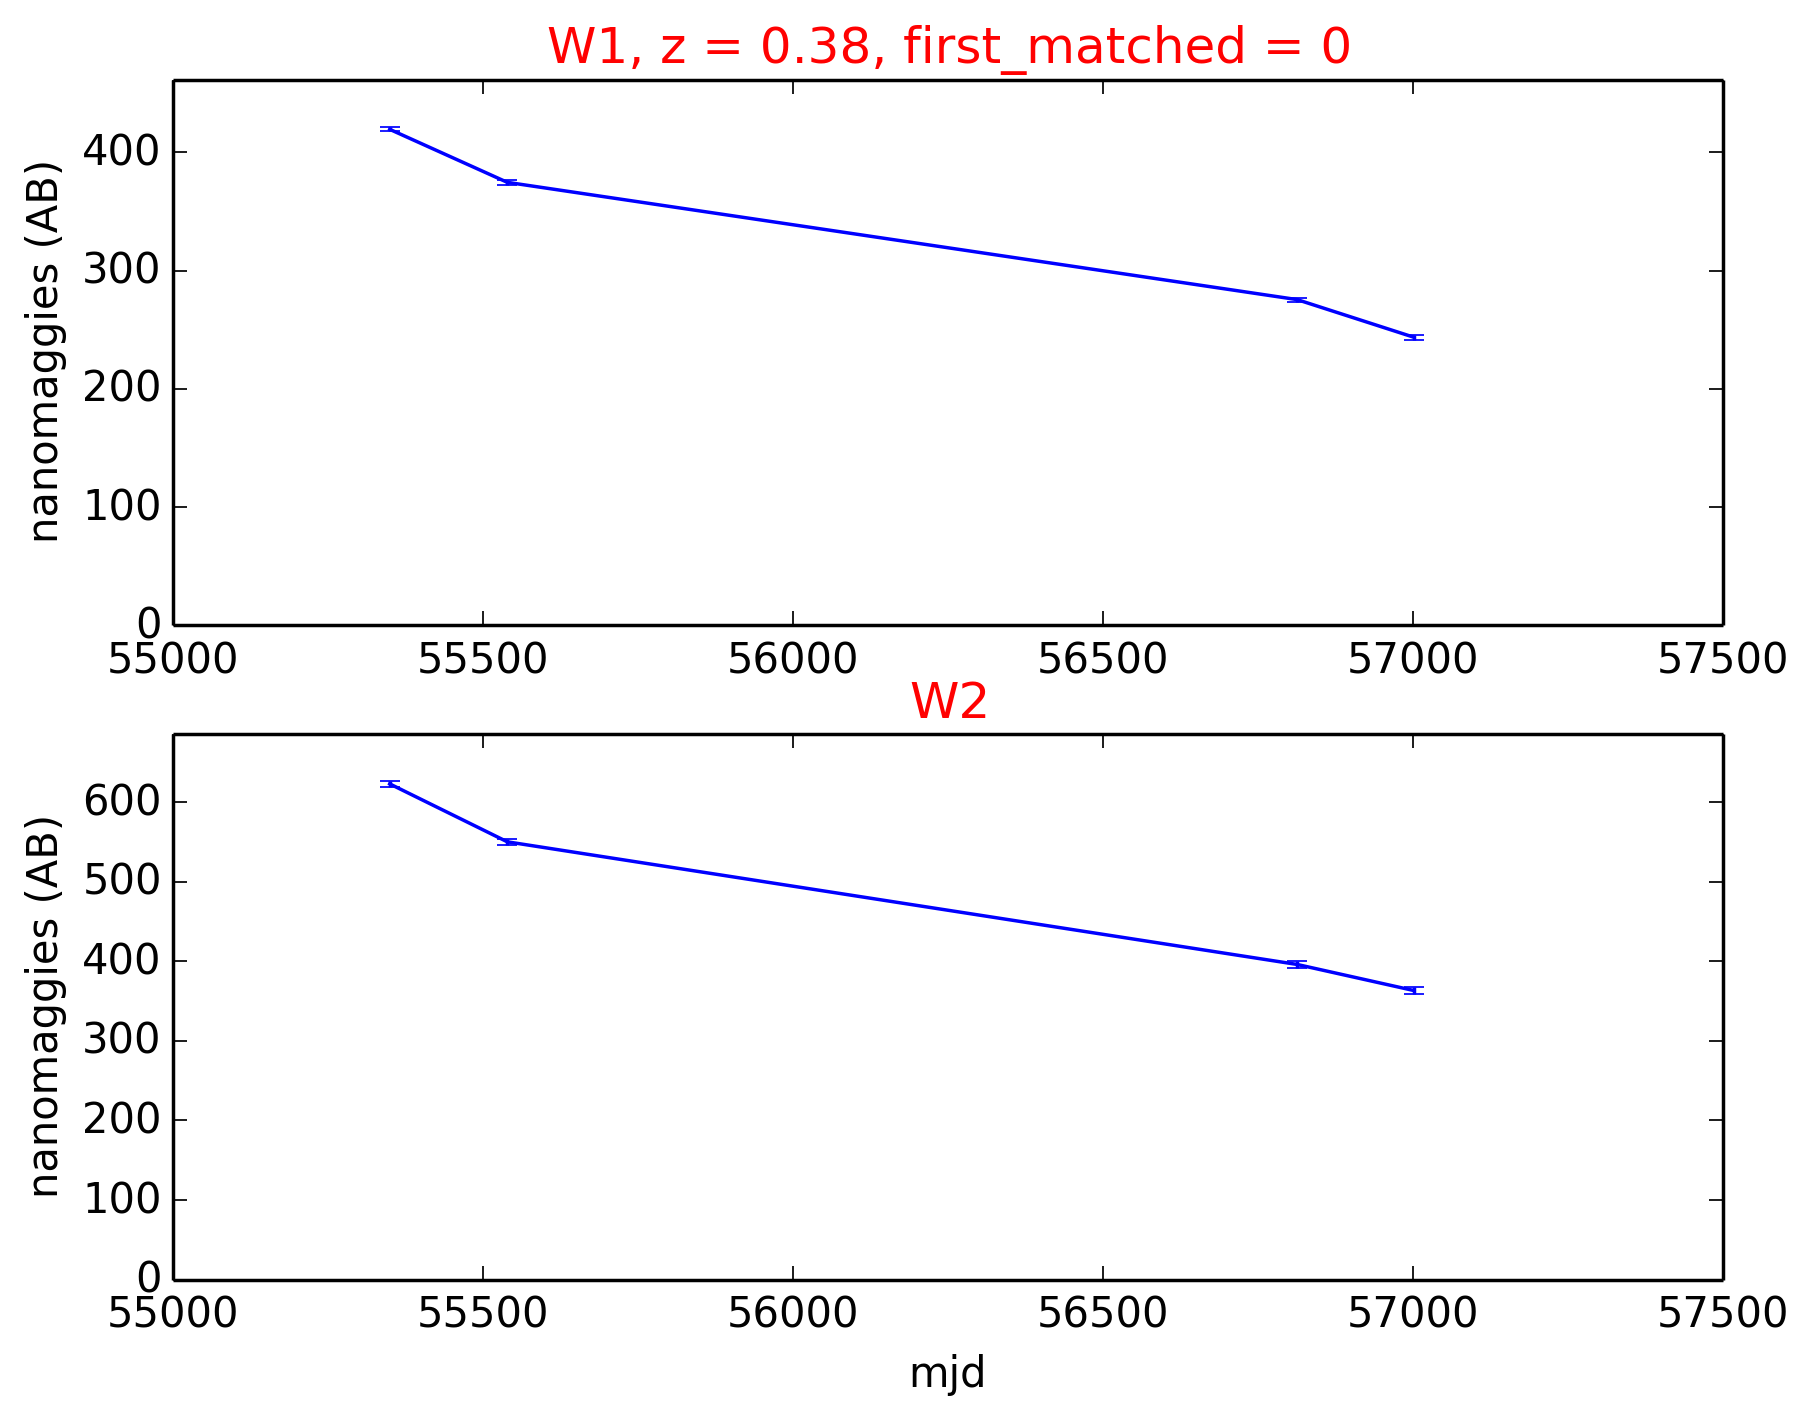
\includegraphics[width=8.00cm, height=6.50cm, 
    trim=0.0cm 0.0cm 0.0cm 0.0cm, clip]
    {../plots/lc/lc_110057p71-005304p5.png}
    \centering
    \caption[]{WISE infrared light-curve for J110057. }
    \label{fig:lc_J110057}
\end{figure}
  
\begin{figure*}
   %% trim=l b r t 
    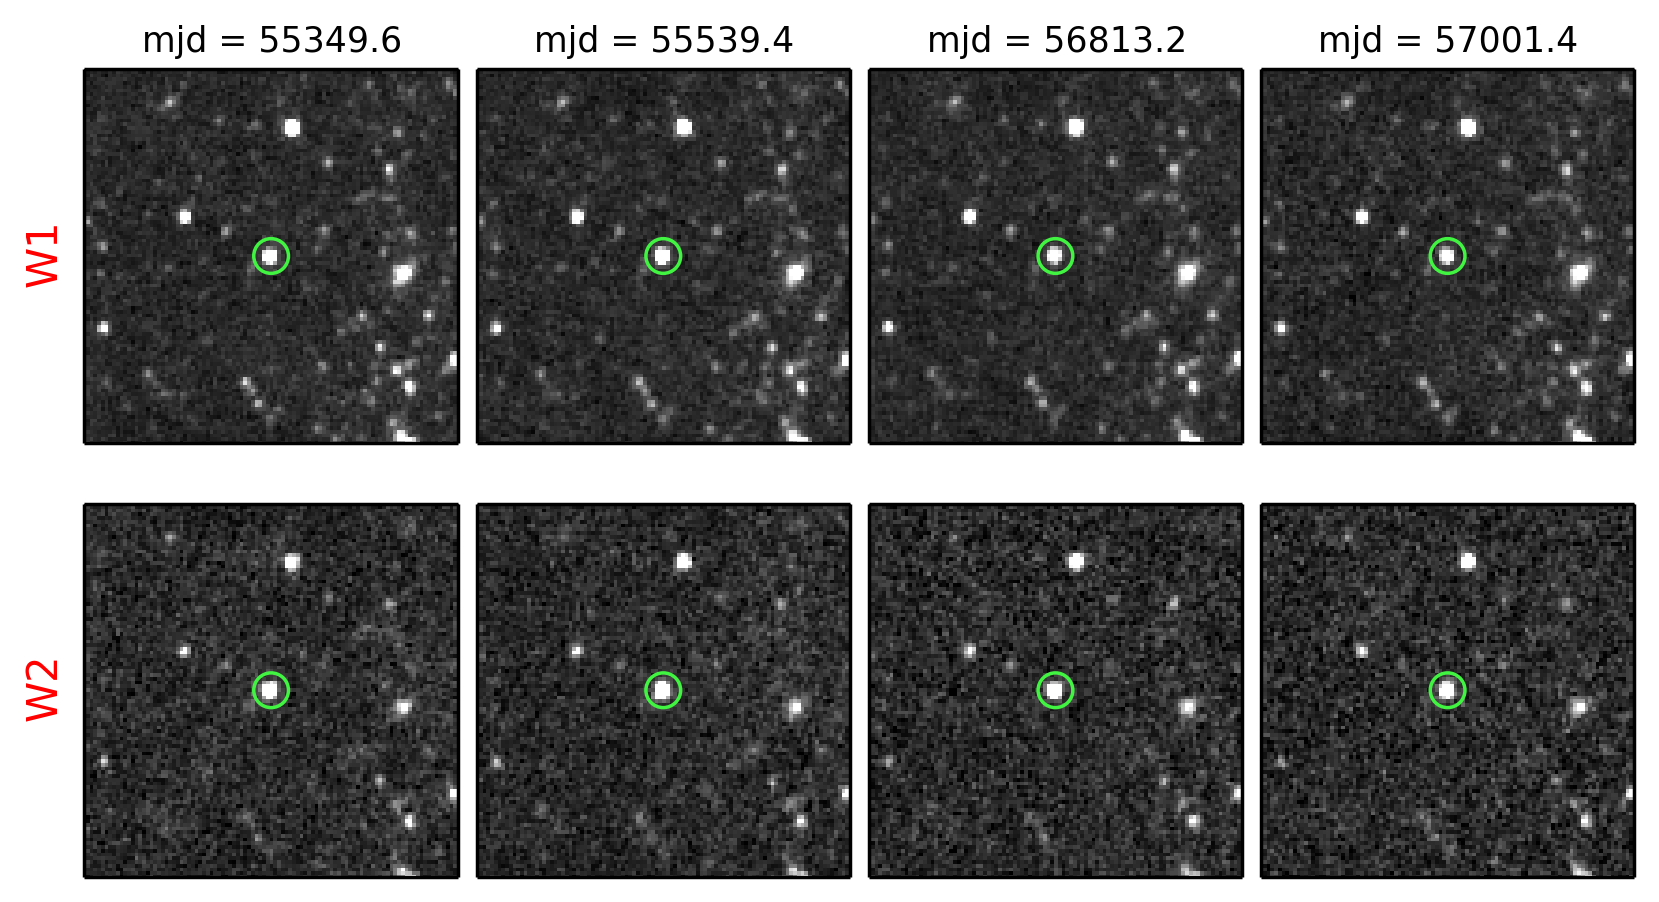
\includegraphics[width=14.00cm, height=7.50cm, 
    trim=0.0cm 0.0cm 0.0cm 0.0cm, clip] 
    {../plots/finder/finder_110057p71-005304p5.png}
    \centering
    % \vspace{-16pt}
    \caption[]{WISE thumbnail images for J110057. }
    \label{fig:finder_J110057}
\end{figure*}

\section{Results: Individual Objects}
Having placed the IR variable quasars in context with their parent 
population, we now turn our attention to objects with particularly interesting 
features, using due to having repeat spectroscopy available. 

The object SDSS J105203.55+151929.4 is one of the IR variable sample 
and is the first CLQ to be discovered through its IR properties. 
Stern et al. (2017, in prep.) has a detailed study of that object. 

In this paper, we will turn our focus to another very interesting object, 
SDSS J110057.71-005304.5. 

\begin{figure*}
  %% trim=l b r t 
  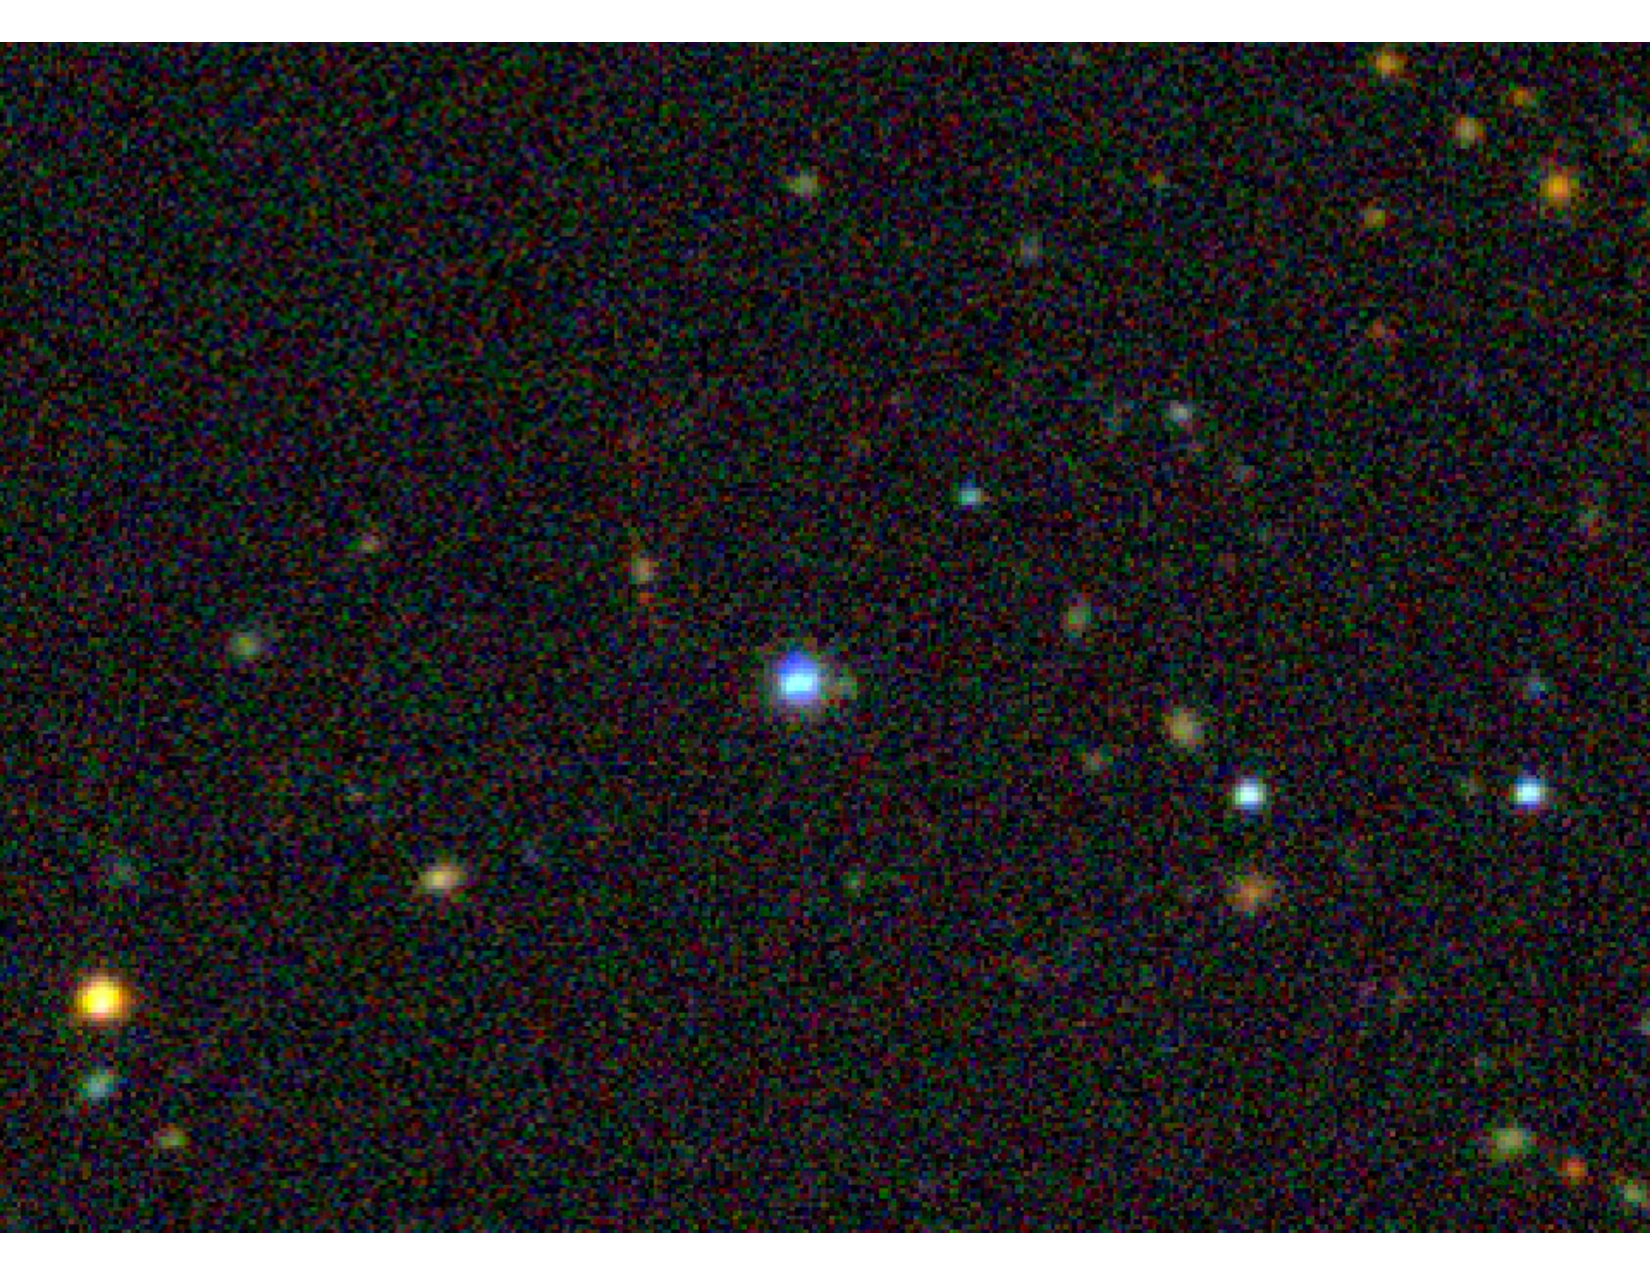
\includegraphics[width=8.50cm, height=6.50cm, trim=0.0cm 0.0cm 0.0cm 0.0cm, clip]
  {../images/J110057_sdss_image_nolabels.pdf}
  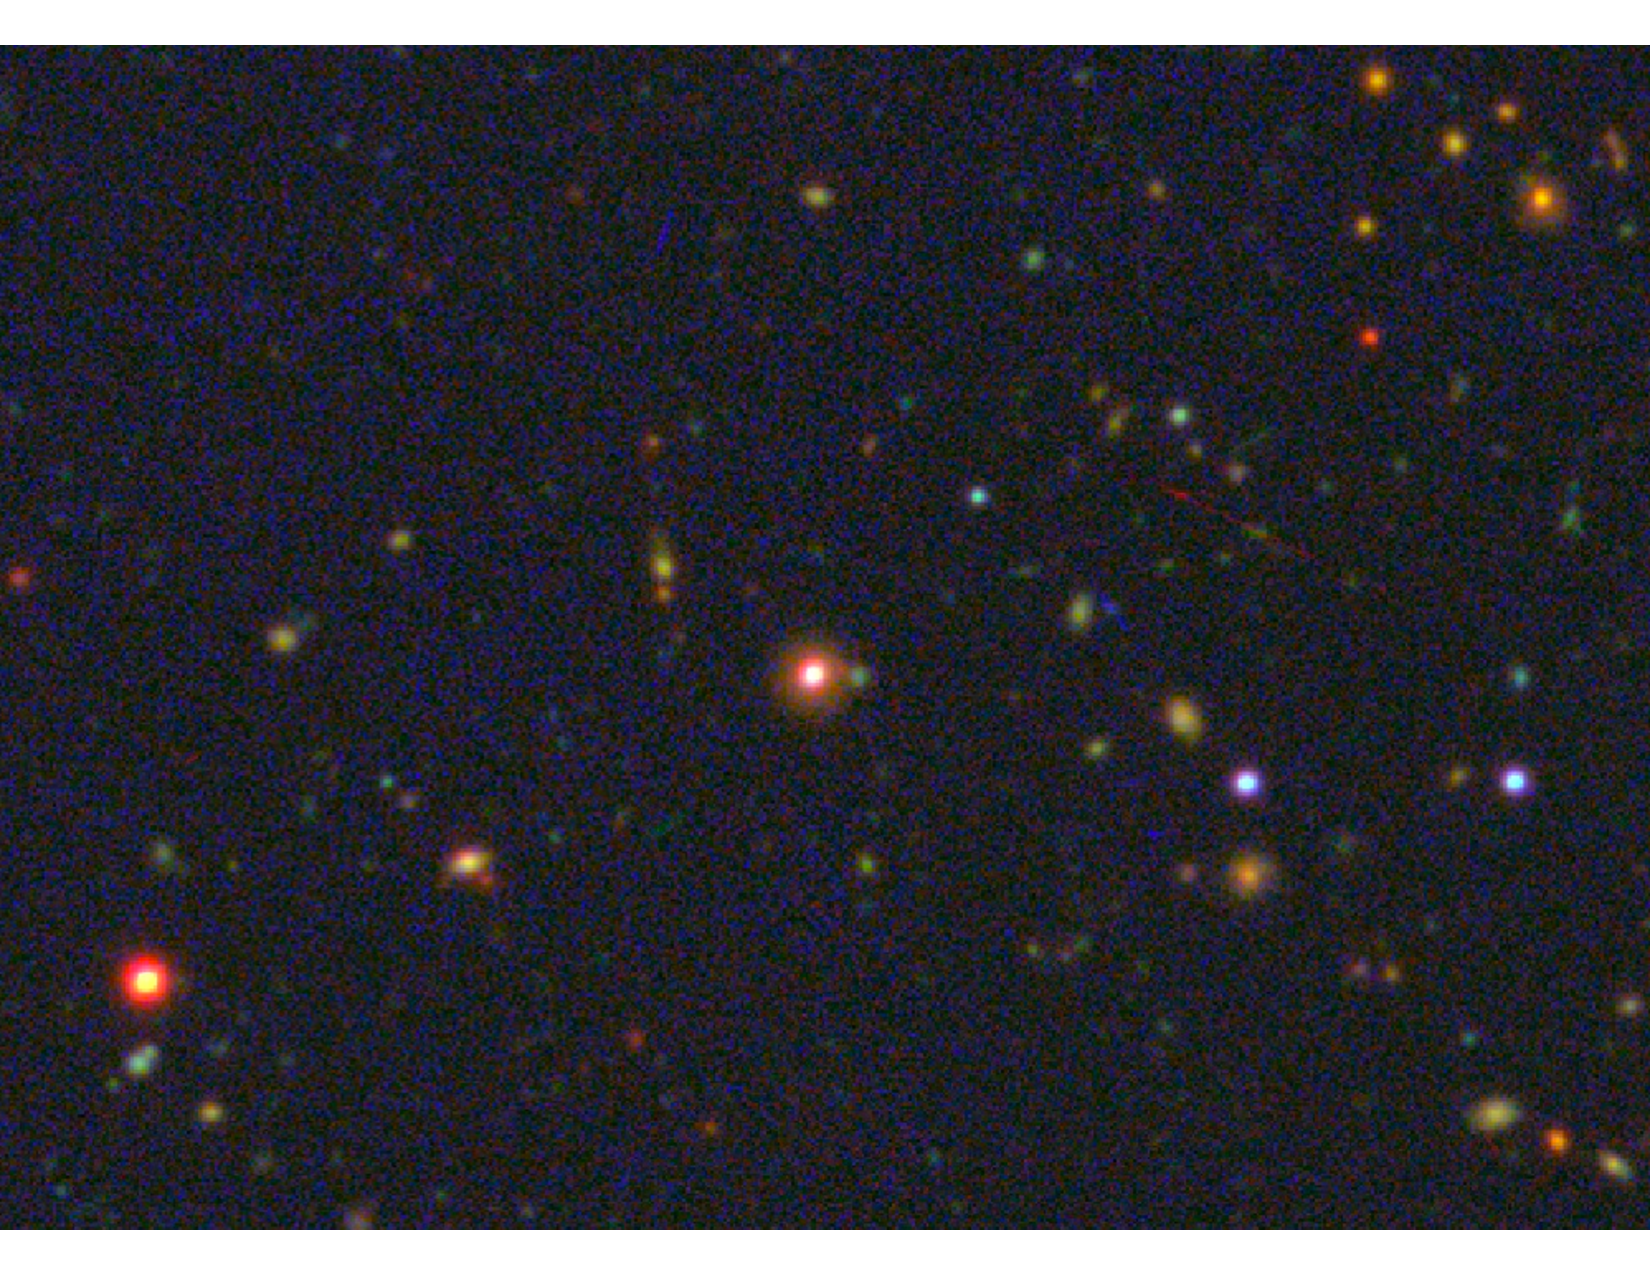
\includegraphics[width=8.50cm, height=6.50cm, trim=0.0cm 0.0cm 0.0cm 0.0cm, clip]
  {../images/J110057_decals_image_nolabels.pdf}
  \centering
  % \vspace{-16pt}
  \caption[]{The SDSS ({\it left} and DECaLS ({\it right}) image of SDSS J110057.71-005304.5 (center). } 
\label{fig:w1100m0052_sdss}
\end{figure*}
\subsection{SDSS J110057.71-005304.5}
Figures~\ref{fig::lc_J110057} presents the IR NEOWISER light curve for 
J110057, and~\ref{fig:finder_J110057} the IR finding charts. 

SDSS J110057.71-005304.5, hereafter J110057, was discovered by 
the Sloan Digital Sky Survey in 2000. 
 J110057 was imaged in Run 756 (which makes up Stripe 10), 
and satisfied a number of spectroscopic targeting flags
\footnote{SERENDIP\_BLUE, ROSAT\_D,  ROSAT\_C,  ROSAT\_B, QSO\_SKIRT, ROSAT\_A, 
see \citet{EDR} and \citet{Richards02} for flag descriptions.}
making it a quasar target. A spectrum was obtain on MJD 51908, on Plate 
277, Fiber 212, and the spectrum of a $z=0.378\pm0.00003$ was

In the DECaLS, the DECaLS brick containing J110057.71-005304.5.
There are 8, 3 and 9 exposures in the $g-$, $r-$ and $z-$band 
respectively. 
$56707.146 \leq g_{\rm MJD} \leq  56727.201$;  
$56367.091 \leq  r_{\rm MJD} \leq  56367.230$; 
$56383.159 \leq  z_{\rm MJD} \leq  57398.350$. 

As can be seen, the $g-$ and $r-$band observations have fairly limited
time spans, and are separated by roughly a year. The $z$-band
observations span almost 3 years.  The DESI imaging brick name is
1651m010.
%%  I've attached the CCDs file, which comes from:
%%  /project/projectdirs/cosmo/data/legacysurvey/dr3.1/coadd/165/1651m010/legacysurvey-1651m010-ccds.fits

Second epoch spectrum is from BOSS and has a dramatic downturn at 
$\lesssim$4300\AA\ . 

A third epoch spectrum was obtained from the Palomar 5m 
telescope using the DBSP instrument. 
Two exposures of 600s+300s were taken in good conditions. 
%%
Feature to note include: the continuum straddling MgII
being blue in the 2017 spectrum, as it was for the SDSS spectrum in 2000, as opposed to
red, as it was for the BOSS spectrum in 2010.  

Lorem ipsum dolor sit amet, consectetur adipiscing elit. Aliquam porta
sodales est, vel cursus risus porta non. Vivamus vel pretium
velit. Sed fringilla suscipit felis, nec iaculis lacus convallis
ac. Fusce pellentesque condimentum dolor, quis vehicula tortor
hendrerit sed. Class aptent taciti sociosqu ad litora torquent per
conubia nostra, per inceptos himenaeos. Etiam interdum tristique diam
eu blandit. Donec in lacinia libero.

Sed elit massa, eleifend non sodales a, commodo ut felis. Sed id
pretium felis. Vestibulum et turpis vitae quam aliquam convallis. Sed
id ligula eu nulla ultrices tempus. Phasellus mattis erat quis metus
dignissim malesuada. Nulla tincidunt quam volutpat nibh facilisis
euismod. Cras vel auctor neque. Nam quis diam risus.

Nunc semper quam et leo interdum vulputate eu quis magna. Sed nec arcu
at orci egestas convallis. Aenean quam velit, aliquam vitae viverra
in, elementum vel elit. Nunc suscipit aliquet sapien a suscipit. Cras
nulla ipsum, posuere eu fringilla sit amet, dapibus ultricies
nulla. Nullam eu augue id purus mollis dignissim sed et
libero. Phasellus eget justo sed neque pellentesque egestas nec id
arcu. Donec facilisis pulvinar sapien et fringilla. Suspendisse
vestibulum rhoncus sapien id laoreet. Morbi et orci vitae tortor
imperdiet imperdiet. In hac habitasse platea dictumst. Vivamus vel
neque id mi ultrices tristique. Integer quam libero, ornare vel
gravida in, feugiat a ante. Nam dapibus, tellus vitae pellentesque
cursus, dui nisl egestas augue, non fermentum nisl est nec
nisi. Vestibulum nec mi justo, eget dapibus velit.
\begin{figure*}
  %% trim=l b r t 
  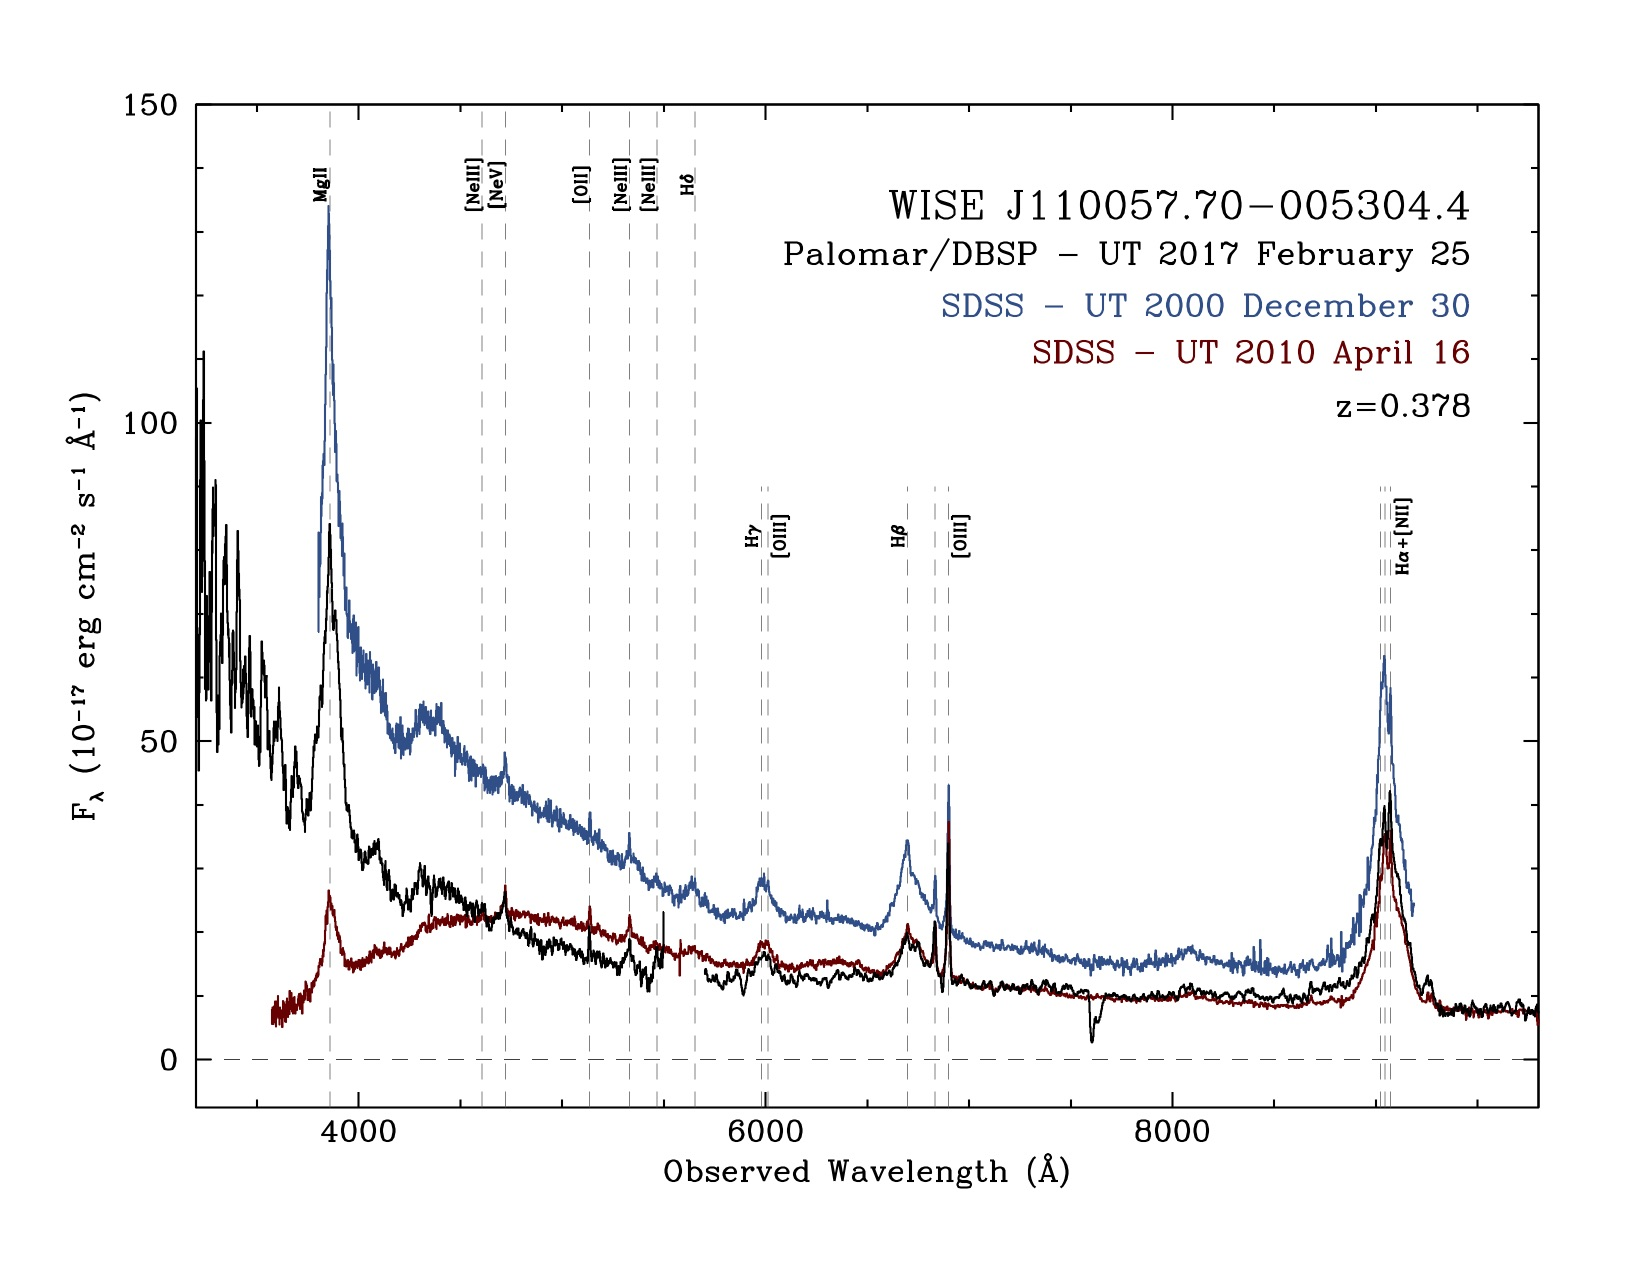
\includegraphics[width=17.00cm, height=9.50cm, trim=0.0cm 0.0cm 0.0cm 0.0cm, clip]
  {../plots/spectra/w1100m0052_sdss.jpg}
  \centering
  % \vspace{-16pt}
  \caption[]{  } 
\label{fig:w1100m0052_sdss}
\end{figure*}

\begin{figure}
  %% trim=l b r t 
  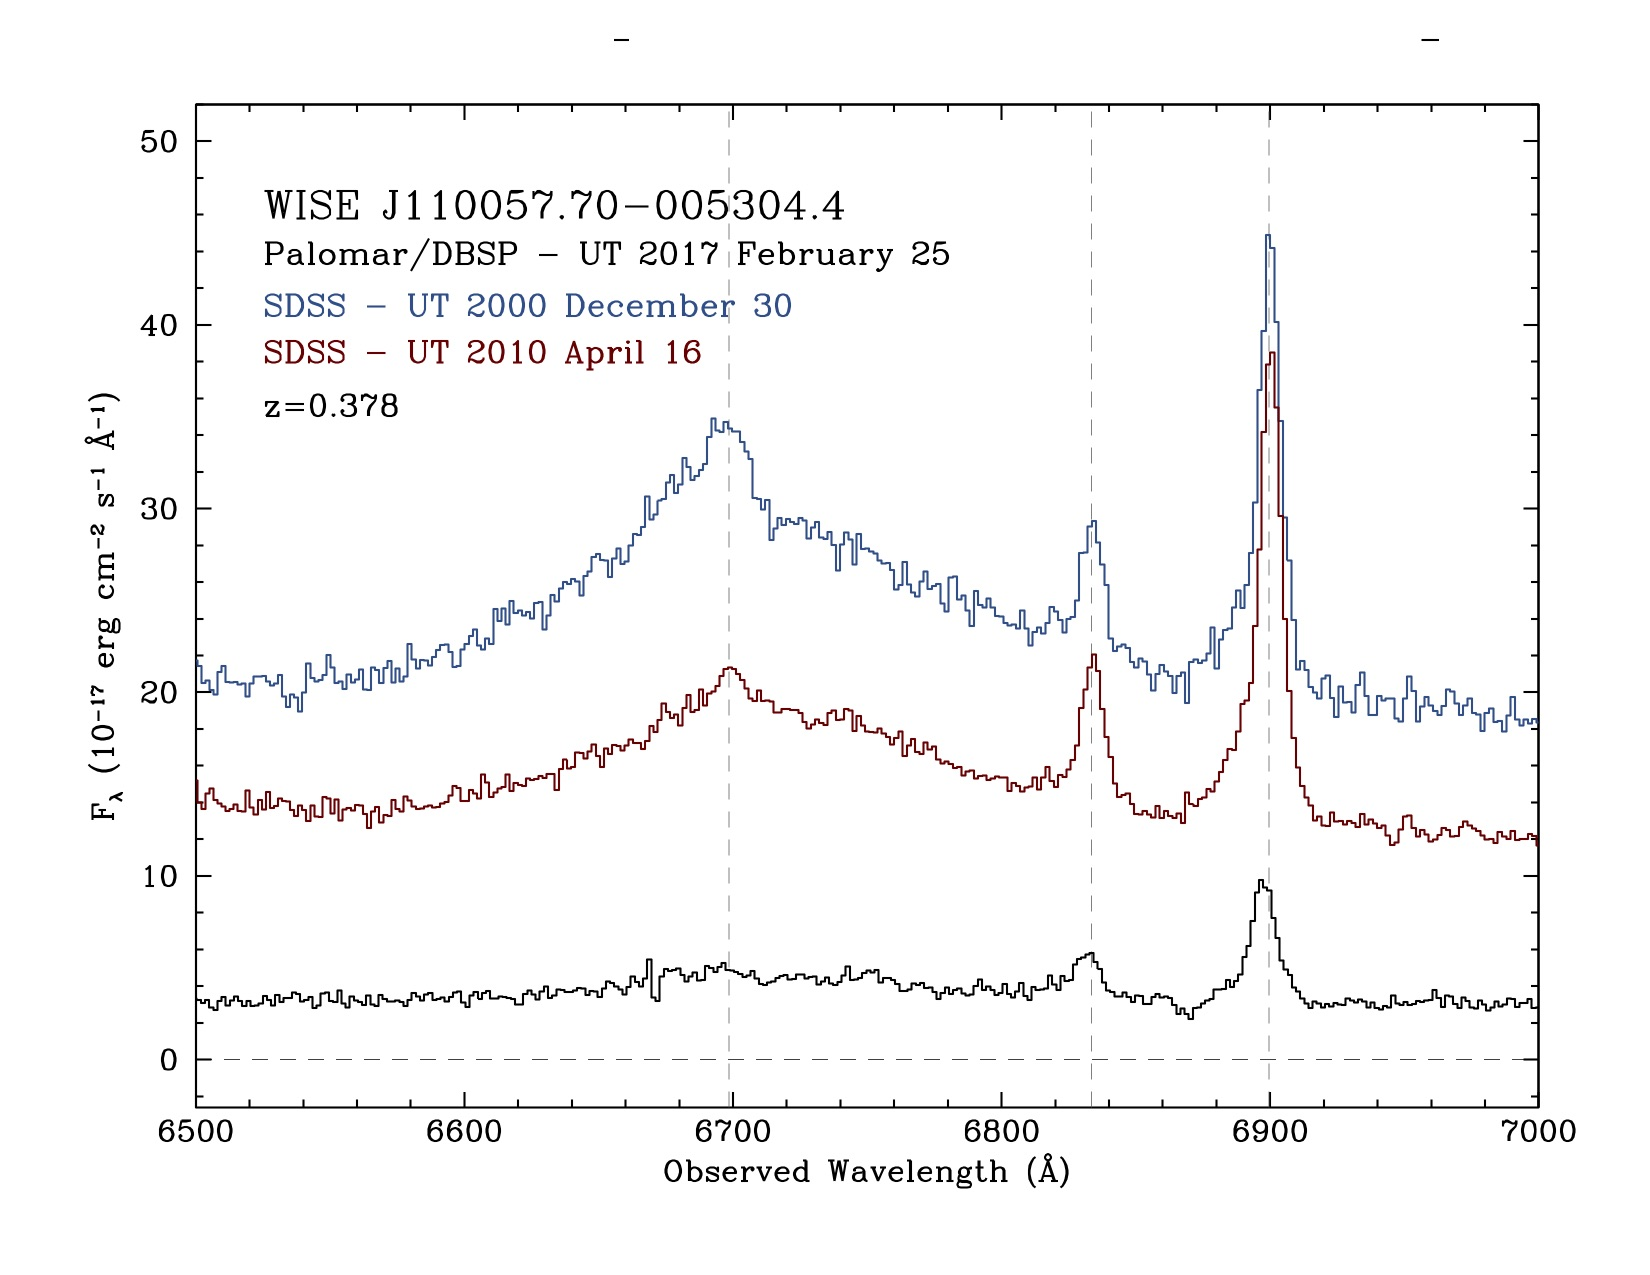
\includegraphics[width=8.00cm, height=7.50cm, trim=0.0cm 0.0cm 0.0cm 0.0cm, clip]
  {../plots/spectra/w1100m0052_hbeta.jpg}
  \centering
  % \vspace{-16pt}
  \caption[]{SDSS J110057.71-005304.5 H$\beta$ zoom-in.}
 \label{fig:w1100m0052_hbeta}
\end{figure}

\begin{figure}
  %% trim=l b r t 
  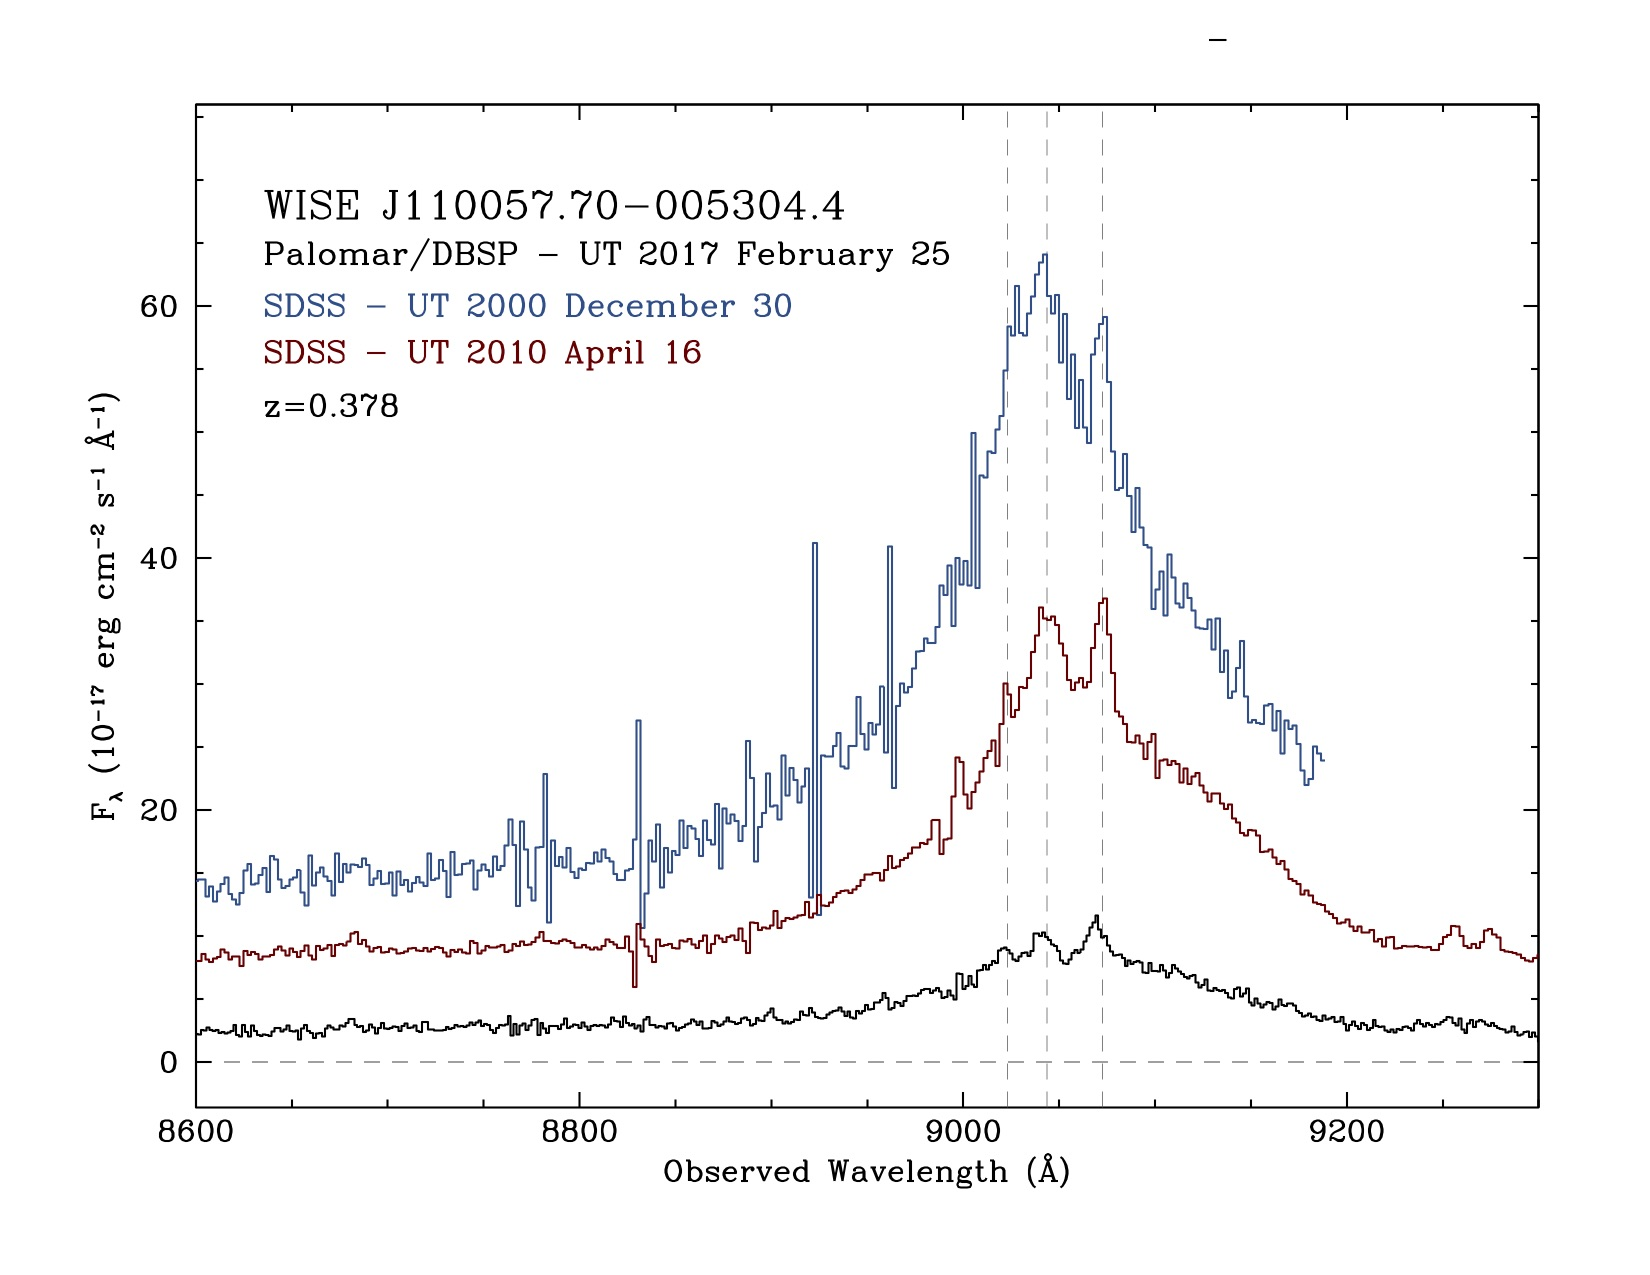
\includegraphics[width=8.00cm, height=7.50cm, trim=0.0cm 0.0cm 0.0cm 0.0cm, clip]
  {../plots/spectra/w1100m0052_halpha.jpg}
  \centering
  % \vspace{-16pt}
  \caption[]{SDSS J110057.71-005304.5 H$\alpha$ zoom-in.}
 \label{fig:w1100m0052_halpha}
\end{figure}



%%%%%%%%%%%%%%%%%%%%%%%%%%%%%%%%%%%%%%%%%%%%%%%%%%%%%%%%%%%%%%
%%%%%%%%%%%%%%%%%%%%%%%%%%%%%%%%%%%%%%%%%%%%%%%%%%%%%%%%%%%%%%
%%
%%     S E C T I O N     5      S E C T I O N     5       S E C T I O N     5       S E C T I O N     5
%%     S E C T I O N     5      S E C T I O N     5       S E C T I O N     5       S E C T I O N     5  
%%     S E C T I O N     5      S E C T I O N     5       S E C T I O N     5       S E C T I O N     5  
%%
%%%%%%%%%%%%%%%%%%%%%%%%%%%%%%%%%%%%%%%%%%%%%%%%%%%%%%%%%%%%%%
%%%%%%%%%%%%%%%%%%%%%%%%%%%%%%%%%%%%%%%%%%%%%%%%%%%%%%%%%%%%%%
\section{Discussion}
In the above sections, we placed the variable IR quasar sample in context to 
the parent quasar population. We also discussed SDSS J110057.71-005304.5 
as a standout solo object. In this section, we model the observed properties 
of J110057 to understand its central engine properties. We then attempt to 
link the IR Variability to the Changing Look phenomena in general. 

\subsection{Modeling the IR light-curves and the optical spectra of J110057}
Nunc semper quam et leo interdum vulputate eu quis magna. Sed nec arcu
at orci egestas convallis. Aenean quam velit, aliquam vitae viverra
in, elementum vel elit. Nunc suscipit aliquet sapien a suscipit. Cras
nulla ipsum, posuere eu fringilla sit amet, dapibus ultricies
nulla. Nullam eu augue id purus mollis dignissim sed et
libero. Phasellus eget justo sed neque pellentesque egestas nec id
arcu. Donec facilisis pulvinar sapien et fringilla. Suspendisse
vestibulum rhoncus sapien id laoreet. Morbi et orci vitae tortor
imperdiet imperdiet. In hac habitasse platea dictumst. Vivamus vel
neque id mi ultrices tristique. Integer quam libero, ornare vel
gravida in, feugiat a ante. Nam dapibus, tellus vitae pellentesque
cursus, dui nisl egestas augue, non fermentum nisl est nec
nisi. Vestibulum nec mi justo, eget dapibus velit.

\subsection{Linking IR Variability to the Changing Look phenomena}
Sed sed ipsum diam. In risus tortor, sagittis eu auctor in, varius in dui. Mauris a nunc ut ligula ullamcorper tincidunt. Nunc aliquam eros ac risus pellentesque aliquam. Phasellus augue velit, varius at porttitor sit amet, pretium eget felis. Ut mollis tellus elementum magna porttitor rutrum. Etiam blandit leo eget est consectetur imperdiet. Quisque et diam nec orci vulputate varius vitae id sapien.

Donec elit tortor, scelerisque ac molestie id, hendrerit sit amet ipsum. Maecenas non tempus sem. Pellentesque ut enim velit, eu sagittis elit. Nulla in elementum erat. In dictum arcu at nisi porttitor commodo. Donec felis felis, elementum sit amet ultrices ac, interdum nec ante. Nullam eget faucibus lectus. Donec vitae eros sapien, et faucibus ligula. Aenean pharetra viverra fermentum.





%%%%%%%%%%%%%%%%%%%%%%%%%%%%%%%%%%%%%%%%%%%%%%%%%%%%%%%%%%%%%%
%%%%%%%%%%%%%%%%%%%%%%%%%%%%%%%%%%%%%%%%%%%%%%%%%%%%%%%%%%%%%%
%%
%%     S E C T I O N     6      S E C T I O N     6       S E C T I O N     6       S E C T I O N     6
%%     S E C T I O N     6      S E C T I O N     6       S E C T I O N     6       S E C T I O N     6  
%%     S E C T I O N     6      S E C T I O N     6       S E C T I O N     6       S E C T I O N     6 
%%
%%%%%%%%%%%%%%%%%%%%%%%%%%%%%%%%%%%%%%%%%%%%%%%%%%%%%%%%%%%%%%
%%%%%%%%%%%%%%%%%%%%%%%%%%%%%%%%%%%%%%%%%%%%%%%%%%%%%%%%%%%%%%
\section{Discussion and Conclusions}
Sed non felis iaculis dui iaculis mattis facilisis ullamcorper
ipsum. Donec erat nunc, consectetur et ornare in, egestas vitae
mauris. Praesent suscipit rutrum purus, in interdum tellus euismod sit
amet. Nulla facilisi. Etiam nisl ligula, vehicula at fringilla et,
sagittis eu odio.

Our conclusions are thus: 
\begin{itemize}
    \item{Hendrerit pretium commodo. Cras dapibus fringilla dolor a
        ultrices. Morbi bibendum neque in magna pellentesque rhoncus. Sed
        vitae lorem lacus.}
    \item{Pellentesque nec justo et dolor scelerisque
        fermentum. Vivamus augue libero, fermentum id tristique at, suscipit
        ultricies turpi.}
    \item{Cras in laoreet mauris. Vivamus nec nulla a dui commodo
        adipiscing. Proin vulputate lectus nec arcu iaculis sit amet auctor
        ligula ultricies. Phasellus condimentum gravida tincidunt. Phasellus
        et mauris ac nibh vestibulum vehicula.}
\end{itemize}

Morbi et augue id purus gravida sagittis quis in sem. Phasellus quis
risus bibendum eros luctus auctor. Proin non tempus velit. Etiam
laoreet, enim nec scelerisque dictum, tortor massa tempor enim, id
pretium justo quam ac lectus. Maecenas diam nibh, interdum at lobortis
sit amet, dignissim et quam. Sed tincidunt faucibus risus, congue
tempus nisl consectetur eget. Suspendisse venenatis turpis ut risus
aliquam interdum. In at velit sed ligula dictum dignissim ut et
dui. Curabitur ac scelerisque purus.



\section{Acknowledgments}
We thank the IPAC team for the Explanatory Supplement to the WISE
All-Sky and AllWISE Data Release Products resource.  NEOWISE and
NEOWISE-R makes use of data from WISE, which is a joint project of the
University of California, Los Angeles, and the Jet Propulsion
Laboratory/California Institute of Technology, and NEOWISE, which is a
project of the Jet Propulsion Laboratory/California Institute of
Technology. WISE and NEOWISE are funded by the National Aeronautics
and Space Administration.

This research made use of the NASA Astrophysics Data System.  This
research also made use of the \href{www.astropy.org}{\tt astropy.org}
codebase (proper citation).  The data and code used herein will become
publicly available at \href{\tt
http://www.legacysurvey.org/dr3/Extreme_wise_quasars/} upon
publication of the paper.

N.P.R. acknowledges support from the STFC and the Ernest Rutherford
Fellowship scheme.
%N.P.R. thanks Nathan Bourne for useful discussions on infrared-to-radio flux ratios. 

Funding for the SDSS and SDSS-II has been provided by the Alfred
P. Sloan Foundation, the Participating Institutions, the National
Science Foundation, the US Department of Energy, the National
Aeronautics and Space Administration, the Japanese Monbukagakusho, the
Max Planck Society, and the Higher Education Funding Council for
England. The SDSS web site is
\href{http://www.sdss.org/}{http://www.sdss.org}.

Funding for SDSS-III has been provided by the Alfred P. Sloan
Foundation, the Participating Institutions, the National Science
Foundation, and the U.S. Department of Energy. The SDSS-III web site
is \href{http://www.sdss3.org/}{http://www.sdss3.org/}.  SDSS-III is
managed by the Astrophysical Research Consortium for the Participating
Institutions of the SDSS-III Collaboration including the University of
Arizona, the Brazilian Participation Group, Brookhaven National
Laboratory, University of Cambridge, University of Florida, the French
Participation Group, the German Participation Group, the Instituto de
Astrofisica de Canarias, the Michigan State/Notre Dame/JINA
Participation Group, Johns Hopkins University, Lawrence Berkeley
National Laboratory, Max Planck Institute for Astrophysics, New Mexico
State University, New York University, Ohio State University,
Pennsylvania State University, University of Portsmouth, Princeton
University, the Spanish Participation Group, University of Tokyo,
University of Utah, Vanderbilt University, University of Virginia,
University of Washington, and Yale University.  \\ {\it Facilities:
SDSS, BOSS, WISE, CTIO Blanco+DECam}



\clearpage
\appendix
\section{Technical Details}
All good papers have to have an Appendix. 

\begin{table}[ht]
\centering
\begin{tabular}{l l l}
\hline\hline
\hline
SDSS Info  &	   Description	&			Example \\
\hline
SDSSJ  	      &   SDSS object name	&		000920.76+033021.7 \\
RA    	      &	   SDSS object R.A. (J2000)&		002.33654086687\\
DEC   	&	   SDSS object Decl.(J2000)	&	+003.50603303134\\
Z  	&	   SDSS (pipeline) redshift &		0.432505905628\\
MJD   &		   Modified Julian Date&			55806\\
FIBER   &	   Fiber number		&		0196\\
PLATE   &	   Plate number		&		4297\\
U\_FLUX   &	   u-band flux		&		10.1695\\
G\_FLUX   	 &  g-band flux		&		13.8142\\
R\_FLUX   	&   r-band flux		&		14.1181\\
I\_FLUX   	&   i-band flux		&		16.7872\\
Z\_FLUX   	 &  z-band flux		&		21.7649\\
DR     &		   Data Release number&			12\\
FIRST\_MATCHED  &	   Matched in FIRST radio survey?&	0\\
\hline \hline
 WISE LC Metrics & Description			&	Example\\
\hline
MEAN\_SNR\_W1  &	   Mean Signal-to-noise, W1		& 38.8656\\
MEAN\_SNR\_W2   &	   Mean Signal-to-noise, W2	&	22.8657\\
PEARSON\_R   &	   Pearson correlation coefficient &	0.999489\\
N\_EPOCH   &	   number of WISE epochs	&	4\\
NBAD\_W1  &	   Quality flag for epochs??&		0\\
NBAD\_W2  &	   Quality flag for epochs??&		0\\
MONO\_W1   &	   a	   	    		&	1\\
MONO\_W2  &	   b				&	1\\
BEST\_FLUX\_W1  & 	   c		&			72.078\\
BEST\_FLUX\_W2   &	   d		&			94.7315\\
CHI2\_W1      &	   e			&		170.705\\
CHI2\_W2      &	   f			&		88.7313\\
RCHI2\_W1   &	   g			&		56.9016\\
RCHI2\_W2   &	   h			&		29.5771\\
FLUX\_MIN\_W1   &	   i		&			56.8723\\
FLUX\_MAX\_W1   &	   j		&			86.1033\\
FLUX\_MIN\_W2   &	   k		&			69.1232\\
FLUX\_MAX\_W2   &	   l		&			114.478\\
MAG\_RANGE\_W1  &	   m		&			0.450297\\
MAG\_RANGE\_W2  &	   n		&			0.547747\\
GOOD\_EPOCH\_MASK    o		&			[1 1 1 1 0]\\
RISING\_W1   &	   p			&		0\\
FALLING\_W1  & 	   q		&			1\\
RISING\_W2  &	   r			&		0\\
FALLING\_W2   &	   s		&			1\\
COADD\_ID   &	   t			&		0030p030\\
X\_COADD   &	   u			&		1923.45\\
Y\_COADD   &	   v			&		1648.51\\
\hline \hline
%##Tractor Catalog Format
%##  tractor/<AAA>/tractor-<brick>.fits
%##  http //legacysurvey.org/dr3/catalogs/
Name                 &		   	Description & 	Example\\
\hline
BRICKID		   &	Brick ID [1,662174] & \\
BRICKNAME	   &	Name of brick, near RA=112.6, Dec=+22.2   &   eg "1126p222" \\
OBJID		   &	Catalog object number within this brick; & \\
                            &  a unique identifier hash is BRICKID,OBJID; & \\
                             % OBJID spans [0,N-1] and is contiguously enumerated within each blob & \\
BRICK\_PRIMARY  &	True if the object is within the brick boundary & \\
BLOB		   &	Blend family; & 		contiguously numbered from 0  \\
NINBLOB	  	   &	Number of sources in this BLOB & \\
TYCHO2INBLOB  &	 			Is there a Tycho-2 (very bright) star in this blob?& \\
TYPE		   &			Morphological model  & \\
RA		          &			Right ascension at epoch J2000& \\
RA\_IVAR            &		   	Inverse variance of RA & \\
DEC	                 &	  		Declination at epoch J2000& \\
DEC\_IVAR        &	   		Inverse variance of DEC (no cos term!) & \\
BX		  &		X position of coordinates in brick image stack& \\
BY		&   		Y position) of coordinates in brick image stack& \\
%BX0		&   	X position (0-indexed) of coordinates in brick image stack& \\
%BY0		&   	Y position (0-indexed) of coordinates in brick image stack& \\
%LEFT\_BLOB	   	boolean	 			True if an object center has been optimized to be outside the fitting pixel area
%OUT\_OF\_BOUNDS	  	boolean	 			True for objects whose center is on the brick; less strong of a cut than BRICK\_PRIMARY
%DCHISQ		   	float32[5]	 		Difference in χ² between successively more-complex model fits          PSF, SIMPle, DEV, EXP, COMP. The difference is versus no source.
%EBV		   	float32		mag		Galactic extinction E(B-V) reddening from SFD98, used to compute DECAM\_MW\_TRANSMISSION and WISE\_MW\_TRANSMISSION
%CPU\_SOURCE	   	float32		seconds		CPU time used for fitting this source
%CPU\_BLOB	   	float32		seconds		CPU time used for fitting this blob of sources (all sources in this brick with the same blob number)
%BLOB\_WIDTH	   	int16	 			size of this blob of pixels in brick coordinates, bounding box width
%BLOB\_HEIGHT	   	int16	 			size of this blob of pixels in brick coordinates, bounding box height
%BLOB\_NPIX	   	int32	 			size of this blob of pixels in brick coordinates, number of brick pixels
%BLOB\_NIMAGES	   	int16	 			number of images overlapping this blob
%BLOB\_TOTALPIX	   	int32	 			total number of pixels from all the images overlapping this blob
%DECAM\_FLUX	   	float32[6]	nanomaggies	DECam model flux in ugrizY
%DECAM\_FLUX\_IVAR	   	float32[6]	1/nanomaggies²	Inverse variance oF DECAM\_FLUX
%DECAM\_APFLUX	   	float32[8,6]	nanomaggies	DECam aperture fluxes on the co-added images in apertures of radius [0.5,0.75,1.0,1.5,2.0,3.5,5.0,7.0] arcsec in ugrizY
%DECAM\_APFLUX\_RESID 	float32[8,6]	nanomaggies	DECam aperture fluxes on the co-added residual images
%DECAM\_APFLUX\_IVAR  	float32[8,6]	1/nanomaggies²	Inverse variance oF DECAM\_APFLUX
%DECAM\_MW\_TRANSMISSION	float32[6]	 		Galactic transmission in ugrizY filters in linear units [0,1]
%DECAM\_NOBS		uint8[6]	 		Number of images that contribute to the central pixel in each filter for this object (not profile-weighted)
%DECAM\_RCHI2		float32[6]	 		Profile-weighted χ² of model fit normalized by the number of pixels
%DECAM\_FRACFLUX		float32[6]	 		Profile-weight fraction of the flux from other sources divided by the total flux (typically [0,1])
%DECAM\_FRACMASKED	float32[6]	 		Profile-weighted fraction of pixels masked from all observations of this object, strictly between [0,1]
%DECAM\_FRACIN		float32[6]	 		Fraction of a source's flux within the blob, near unity for real sources
%DECAM\_ANYMASK		int16[6]	 		Bitwise mask set if the central pixel from any image satisfy each condition
%DECAM\_ALLMASK		int16[6]	 		Bitwise mask set if the central pixel from all images satisfy each condition
%DECAM\_PSFSIZE		float32[6]	arcsec		Weighted average PSF FWHM per band
%WISE\_FLUX		float32[4]	nanomaggies	WISE model flux in W1,W2,W3,W4
%WISE\_FLUX\_IVAR		float32[4]	1/nanomaggies²	Inverse variance of WISE\_FLUX
%WISE\_MW\_TRANSMISSION	float32[4]	 		Galactic transmission in W1,W2,W3,W4 filters in linear units [0,1]
%WISE\_NOBS		int16[4]	 		Number of images that contribute to the central pixel in each filter for this object (not profile-weighted)
%WISE\_FRACFLUX		float32[4]	 		Profile-weight fraction of the flux from other sources divided by the total flux (typically [0,1])
%WISE\_RCHI2		float32[4]	 		Profile-weighted χ² of model fit normalized by the number of pixels
%WISE\_LC\_FLUX		float32[5,2]	nanomaggies	analog of WISE\_FLUX, for each of up to five unWISE coadd epochs; W1 and W2 only
%WISE\_LC\_FLUX\_IVAR	float32[5,2]	1/nanomaggies²	analog of WISE\_FLUX\_IVAR, for each of up to five unWISE coadd epochs; W1 and W2 only
%WISE\_LC\_NOBS		int16[5,2]	 		analog of WISE\_NOBS, for each of up to five unWISE coadd epochs; W1 and W2 only
%WISE\_LC\_FRACFLUX	float32[5,2]	 		analog of WISE\_FRACFLUX, for each of up to five unWISE coadd epochs; W1 and W2 only
%WISE\_LC\_RCHI2		float32[5,2]	 		analog of WISE\_RCHI2, for each of up to five unWISE coadd epochs; W1 and W2 only
%WISE\_LC\_MJD		float32[5,2]	 		mean MJD in W1 and W2, for up to five unWISE coadd epochs; 0 means epoch unavailable
%FRACDEV			float32	 			Fraction of model in deVauc [0,1]
%FRACDEV\_IVAR		float32	 			Inverse variance of FRACDEV
%SHAPEEXP\_R		float32		arcsec		Half-light radius of exponential model (>0)
%SHAPEEXP\_R\_IVAR		float32		1/arcsec²	Inverse variance of R\_EXP
%SHAPEEXP\_E1		float32	 			Ellipticity component 1
%SHAPEEXP\_E1\_IVAR	float32	 			Inverse variance of SHAPEEXP\_E1
%SHAPEEXP\_E2		float32	 			Ellipticity component 2
%SHAPEEXP\_E2\_IVAR	float32	 			Inverse variance of SHAPEEXP\_E2
%SHAPEDEV\_R		float32		arcsec		Half-light radius of deVaucouleurs model (>0)
%SHAPEDEV\_R\_IVAR		float32		1/arcsec²	Inverse variance of R\_DEV
%SHAPEDEV\_E1		float32	 			Ellipticity component 1
%SHAPEDEV\_E1\_IVAR	float32	 			Inverse variance of SHAPEDEV\_E1
%SHAPEDEV\_E2		float32	 			Ellipticity component 2
%SHAPEDEV\_E2\_IVAR	float32	 			Inverse variance of SHAPEDEV\_E2
%DECAM\_DEPTH		float32		1/nanomaggies²	For a 5σ point source detection limit, 5/(√DECAM\_DEPTH)5/(DECAM\_DEPTH) gives flux in nanomaggies and −2.5(log10((5/(√DECAM\_DEPTH)−9)−2.5(log10⁡((5/(DECAM\_DEPTH)−9) gives corresponding magnitude
%DECAM\_GALDEPTH		float32		1/nanomaggies²	As for DECAM\_DEPTH but for a galaxy (0.45" exp, round) detection sensitivity
%
\hline\hline
\end{tabular}
\label{table:nonlin}
\end{table}

\section{Spectrophotometry for changing look QSO 3836/55302-258}
All really good papers have more than one Appendix.

\begin{figure*}
  %% trim=l b r t 
  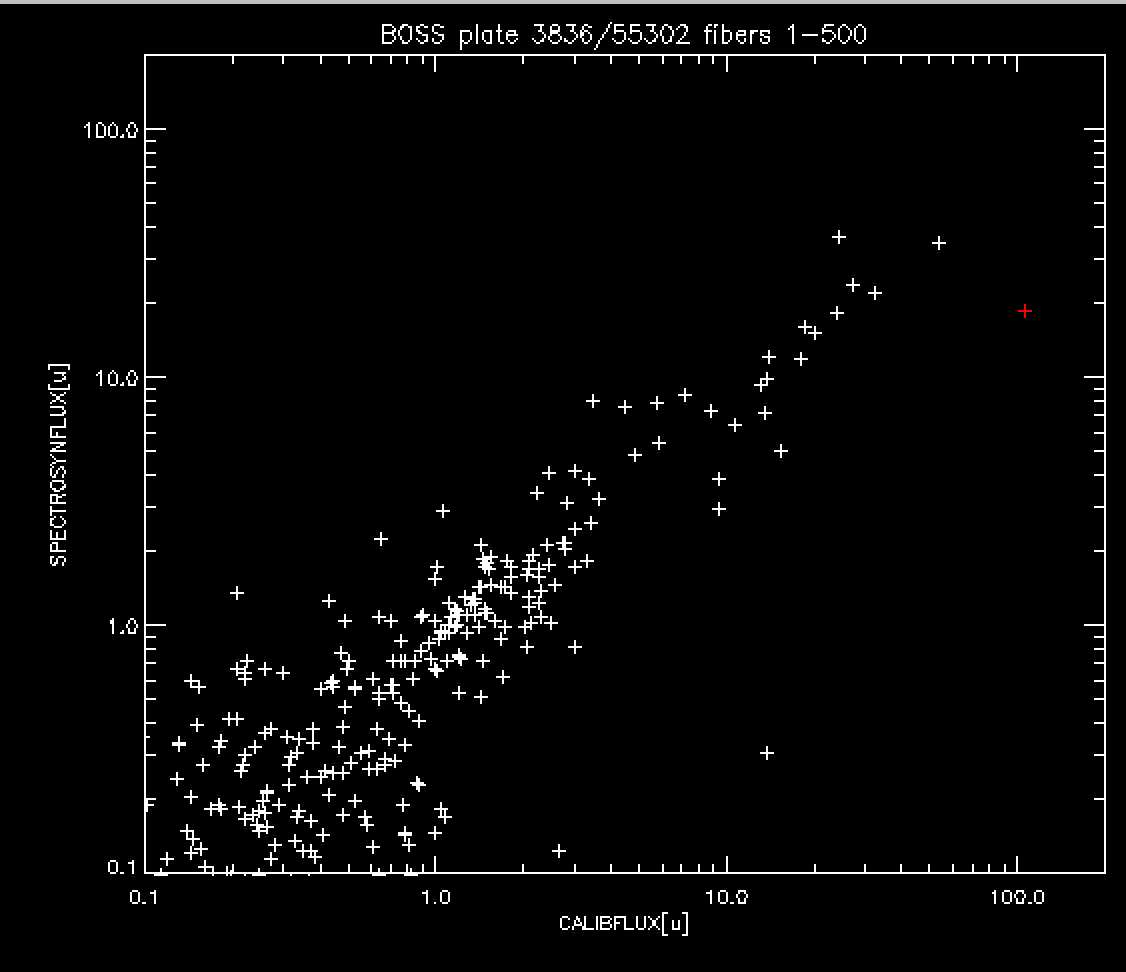
\includegraphics[width=5.80cm, height=6.00cm, trim=0.0cm 0.0cm 0.0cm 0.0cm, clip]
  {../plots/CalibFlux_vs_SpectroSynFlux_uband.png}
  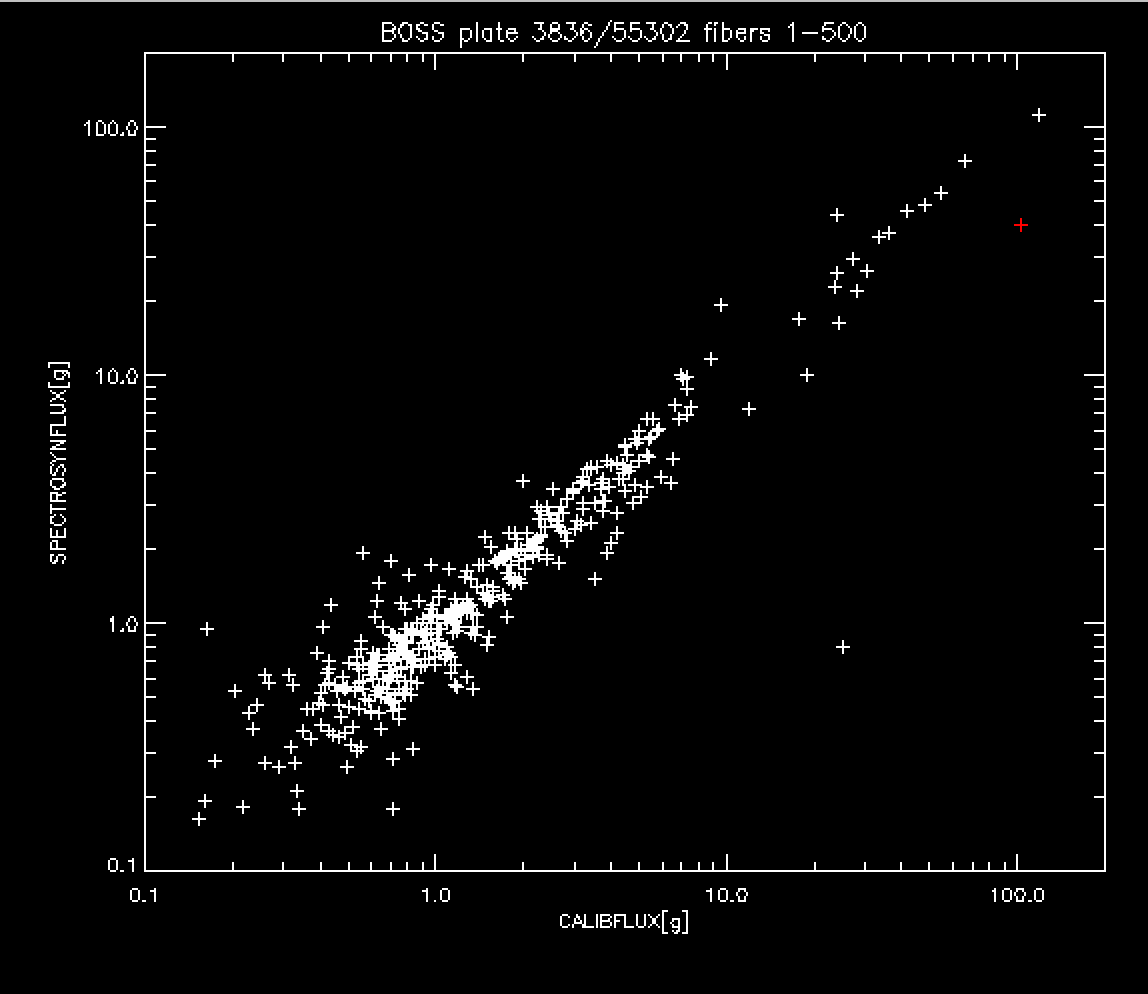
\includegraphics[width=5.80cm, height=6.00cm, trim=0.0cm 0.0cm 0.0cm 0.0cm, clip]
  {../plots/CalibFlux_vs_SpectroSynFlux_gband.png}
  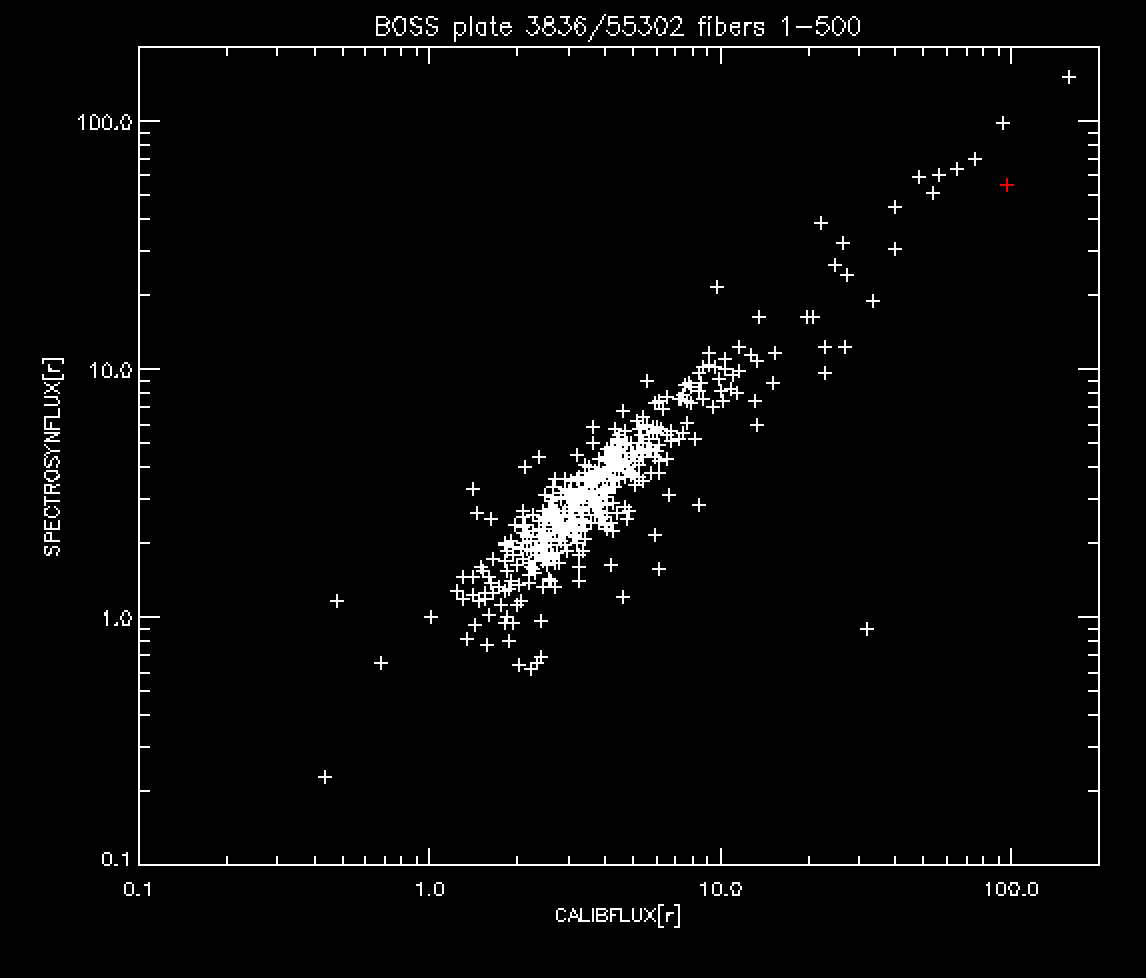
\includegraphics[width=5.80cm, height=6.00cm, trim=0.0cm 0.0cm 0.0cm 0.0cm, clip]
  {../plots/CalibFlux_vs_SpectroSynFlux_rband.png}
  \centering
  % \vspace{-16pt}
  \caption[]{The spectrophotometery checks for Changing Look QSO SDSS J110057. 
    From left to right, the u, g and r bands. 
    Along the x-axis is a measurement of the ``calibration flux'' photometric value 
    which is an estimate of the flux within a 2 arcsecond aperture, and which {\it is} 
    the PSF flux value for point objects (stars). On the $y$-axis is the spectrophotometric
    flux values. For the SDSS $u$, $g$ and $r$-bands from left to right. 
J110057 is the red point, and is clearly off the general trends for the 500 objects 
on this half-plate for one the BOSS spectrographs, but is close to the trend in 
$r$-band strongly suggesting the variations observed in the BOSS spectra are real.} 
 \label{fig:w1100m0052_halpha}
\end{figure*}



\bibliographystyle{mn2e} 
\bibliography{tester_mnras}




\end{document}
